\documentclass[10pt]{beamer}
\usetheme{MonMetropolis}
\setbeamersize{text margin left = 6mm, text margin right = 6mm} 


% Packages ----------------------------------------------------------------------------------------------------------------------

\usepackage[utf8]{inputenc}
\usepackage{booktabs}
\usepackage[scale = 2]{ccicons}
\usepackage{pgfplots}
\usepackage{xspace}
\usepackage{tikz, pgf}
\usepackage{bm}
\usepackage{flowchart}
\usepackage{mathtools}
\usepackage{xcolor}
\usepackage[font = {small, it}]{caption}
\usepackage[cyr]{aeguill}
\usepackage{amsmath, amssymb}
\usepackage{array}
\usepackage[mathscr]{eucal}
\usepackage{eurosym}
\usepackage{subfigure}
\usepackage{color, colortbl}
\usepackage{icomma}
\usepackage[numbers]{natbib}
\usepackage{numprint}
\usepackage{mathrsfs}
\usepackage{fourier} 
\usepackage{makecell}
\usepackage{tabularx, ragged2e}
\usepackage{graphicx}
\usepackage{enumitem}
\usepackage[frenchb]{babel}
\usepackage{tcolorbox}
\usepackage{lipsum}
\usepackage{tabu}
\usepackage{smartdiagram}
\usepackage{algorithmic}
\usepackage{bbm}
\usepackage{xfrac}
\usepackage{algorithm}
\usepackage{algorithm2e}
\usepackage{adjustbox}
\usepackage[most]{tcolorbox}
\usepackage{array}


% TikZ --------------------------------------------------------------------------------------------------------------------------


\tikzstyle{arrow} = [->, line width = 3, > = stealth, color = mgris]
\tikzstyle{ligne} = [--, line width = 3, color = mgris]
\tikzstyle{serpent} = [snake, line width = 3, color = mgris]
\newcommand{\cross}{$\mathbin{\tikz [x = 1ex, y = 1ex, line width = 0.3ex, morange] \draw (0,0) -- (1,1) (0,1) -- (1,0);}$}
\newcommand{\croixrouge}{$\mathbin{\tikz [x = 1ex, y = 1ex, line width = 0.3ex, red] \draw (0,0) -- (1,1) (0,1) -- (1,0);}$}
\newcommand{\trianglevert}{$\mathbin{\tikz [mvert, scale = 1.6] {\pgfuseplotmark{triangle*}}}$}
\newcommand * \circled[1]{\tikz[baseline = (char.base)]{\node[shape = circle, draw, inner sep = 2pt, thick, fill = mgris, color = mgris, text = white, font = \bfseries, scale = 0.8] (char) {#1};}}

\tikzset{curveinscope/.style={every path/.style={draw = red, text=red}}}
\usetikzlibrary{matrix}


% Autres commandes --------------------------------------------------------------------------------------------------------------

\usepgfplotslibrary{dateplot}
\usesmartdiagramlibrary{additions}
\usetikzlibrary{shapes, arrows, chains, arrows.meta, positioning, quotes, matrix, snakes, trees, shadows, calc, shapes.geometric, shapes.misc}
\newcommand\blt{\item[$\bullet$]}
\newcommand\cercle{\item[$\circ$]}
\newcommand\fleche{\item[$\blacktriangleright$]}
\newcommand{\themename}{\textbf{\textsc{metropolis}}\xspace}
\newcommand{\defeq}{\vcentcolon=}
\renewcommand\theadalign{bc}
\renewcommand\theadfont{\bfseries}
\renewcommand\theadgape{\Gape[4pt]}
\renewcommand\cellgape{\Gape[4pt]}
\newcommand{\emphcol}[1]{\textcolor{morange}{#1}}
\newcommand{\argmin}[1]{\underset{#1}{\operatorname{argmin}}\;}
\newcolumntype{?}{!{\vrule width 1pt}}
\SetKwInput{KwInit}{Initialiser}
\DeclareMathOperator*{\moyenne}{moyenne}
\metroset{sectionpage = none}
\colorlet{grispale}{grey!50}
\colorlet{mbleupalepale}{mbleupale!50}


% Page-titre --------------------------------------------------------------------------------------------------------------------

\title{Micro-level loss reserving for general insurance et tentatives d'amélioration \\{\normalfont\normalsize Katrien Antonio et Richard Plat}}
\date{31 janvier 2020} 
\author{Francis Duval\\Manuel Grenier}
\institute{Université du Québec à Montréal}
\titlegraphic{\hspace{-0.35cm}
\includegraphics[width = 2.7cm]{logoUQAM.pdf}}


% Document principal ------------------------------------------------------------------------------------------------------------

\begin{document}
\maketitle

% ----------

\begin{frame}{Contenu}

     \circled{1} Modèle d'Antonio et Plat\\ \vspace{0.6cm}
     \circled{2} Adaptation aux données simulée\\ \vspace{0.6cm}
     \circled{3} Modifications apportées au modèle d'Antonio et Plat -- Francis\\ \vspace{0.6cm}
     \circled{4} Modifications apportées au modèle d'Antonio et Plat -- Manuel\\ \vspace{0.6cm}

\end{frame}

% ----------

\section{Modèle d'Antonio et Plat}

% ----------

\begin{frame}{Rappel sur les micro-réserves}

\begin{figure}
	\centering
		\begin{tikzpicture}[scale = 0.8, color = mgris]
			% Timeline
			\draw[-, very thick] (0,0) -- (7.5,0);
			\draw[->, very thick] (9,0) -- (13.5,0);
			\draw[snake, very thick] (7.5,0) -- (9,0);
	
			\fill (1,0) circle (0.11);
			\node[mvert, scale = 1.6] at (3.5,0) {\pgfuseplotmark{triangle*}};
			\node at (5, 0) {\cross};
			\node at (6.5, 0) {\cross};
			\node at (10, 0) {\cross};
			\fill[mgris] (11.878,-0.122) rectangle (12.122,0.122);
	
			% Vertical arrows
			\draw[->, thick] (1,1.2) -- (1,0.4);
			\node at (1,1.5) {\normalsize Survenance};
			\draw[->, thick] (3.5,1.2) -- (3.5,0.4);
			\node at (3.5,1.5) {\normalsize Déclaration};
			\draw[->, thick] (12,1.2) -- (12,0.4);
			\node at (12,1.5) {\normalsize Fermeture};
	
			% Payments
			\draw [decorate, decoration = {brace, amplitude = 4pt}, thick, yshift = 2] (4.7,0.8) -- (10.3,0.8);
			\node at (7.5,1.5) {\normalsize Paiements};
			\node at (5, 0.5) {\normalsize $P_1$};
			\node at (6.5, 0.5) {\normalsize $P_2$};
			\node at (10, 0.5) {\normalsize $P_M$};
			
			% IBNR and RBNS
			\draw [decorate, decoration = {brace, mirror, amplitude = 4pt}, thick, yshift = -7] (1,-0.3) -- (3.45,-0.3);
			\draw [decorate, decoration = {brace, mirror, amplitude = 4pt}, thick, yshift = -7] (3.55,-0.3) -- (12,-0.3);
			\node at (2.225,-1.1) {\normalsize Délai de déclaration};
			\node at (7.775,-1.1) {\normalsize Processus de développement};
		\end{tikzpicture}
\end{figure}

\begin{exampleblock}{Objectif}
    À la date d'évaluation, on veut prédire le montant total des paiements futurs des réclamations IBNR et RBNS. 
\end{exampleblock}

\end{frame}

% ----------

\begin{frame}{Réclamations IBNR et RBNS}
    
    Pour une date d'évaluation fixe, on peut classer les réclamations en 2 catégories:
    
\begin{figure}
	\centering
		\begin{tikzpicture}[scale = 0.8, color = mgris]
			% Timeline
			\draw[-, very thick] (0,0) -- (7.5,0);
			\draw[->, very thick] (9,0) -- (13.5,0);
			\draw[snake, very thick] (7.5,0) -- (9,0);
	
			\fill (1,0) circle (0.11);
			\node[mvert, scale = 1.6] at (3.5,0) {\pgfuseplotmark{triangle*}};
			\node at (5, 0) {\cross};
			\node at (6.5, 0) {\cross};
			\node at (10, 0) {\cross};
			\fill[mgris] (11.878,-0.122) rectangle (12.122,0.122);
	
			% Vertical arrows
			\draw[->, thick] (1,1.2) -- (1,0.4);
			\node at (1,1.5) {\normalsize Survenance};
			\draw[->, thick] (3.5,1.2) -- (3.5,0.4);
			\node at (3.5,1.5) {\normalsize Déclaration};
			\draw[->, thick] (12,1.2) -- (12,0.4);
			\node at (12,1.5) {\normalsize Fermeture};
	
			% Payments
			\draw [decorate, decoration = {brace, amplitude = 4pt}, thick, yshift = 2] (4.7,0.8) -- (10.3,0.8);
			\node at (7.5,1.5) {\normalsize Paiements};
			\node at (5, 0.5) {\normalsize $P_1$};
			\node at (6.5, 0.5) {\normalsize $P_2$};
			\node at (10, 0.5) {\normalsize $P_M$};
			
			% IBNR and RBNS
			\draw [decorate, decoration = {brace, mirror, amplitude = 4pt}, thick, yshift = -7] (1,-0.3) -- (3.45,-0.3);
			\draw [decorate, decoration = {brace, mirror, amplitude = 4pt}, thick, yshift = -7] (3.55,-0.3) -- (12,-0.3);
			\node at (2.225,-1.1) {\normalsize IBNR};
			\node at (7.775,-1.1) {\normalsize RBNS};
		\end{tikzpicture}
\end{figure}
    
\end{frame}

% ----------

\begin{frame}{Aperçu du modèle}

     \begin{itemize}
         \fleche \textbf{Modèle basé sur un processus de Poisson avec marqueurs.}
         \begin{itemize}
             \cercle Les survenances arrivent selon un processus de Poisson.
             \cercle Un marqueur aléatoire est associé à chaque survenance.
            %  \cercle Ici, le marqueur associé à chaque survenance correspond au couple (délai de déclaration, processus de développement).
         \end{itemize}
         \fleche \textbf{Information au niveau de la réclamation utilisée.}
            \begin{itemize}
                \cercle Date de survenance
                \cercle Délai de déclaration
                \cercle Survenance des paiements et leur sévérité
                \cercle Date de fermeture
                \cercle Caractéristiques des réclamations
            \end{itemize}
         \fleche \textbf{Estimation par maximum de vraisemblance.}
     \end{itemize}

    \begin{exampleblock}{Note}
        Modèle très flexible car construit par blocs. On peut remplacer les blocs et estimer le modèle de la même manière.
    \end{exampleblock}

\end{frame}

% ----------

\begin{frame}{Processus de Poisson avec marqueurs}

    \begin{itemize}
        \onslide<1->{\fleche Dans sa forme la plus simple, un processus de Poisson avec marqueurs se simule comme suit:}
        \begin{itemize}
            \onslide<2->{\cercle On simule d'abord les événements selon un processus de Poisson.}
            \onslide<3->{\cercle Ensuite, on simule le marqueur pour chaque événement.}
        \end{itemize}
    \end{itemize}
    
    \begin{figure}
    	\centering
    	\begin{tikzpicture}[scale = 0.8, color = mgris]
    		\onslide<1->{\draw[->, very thick] (0, 0) -- (13.5, 0);}
    		\onslide<2>{\fill (0.42, 0) circle (0.11);}
    		\onslide<2>{\fill (2.36, 0) circle (0.11);}
    		\onslide<2>{\fill (7.33, 0) circle (0.11);}
    		\onslide<2>{\fill (8.26, 0) circle (0.11);}
    		\onslide<2>{\fill (9.27, 0) circle (0.11);}
    		\onslide<2>{\fill (11.05, 0) circle (0.11);}
    		
    		\onslide<3->{\fill (0.42, 0) circle (0.13);}
    		\onslide<3->{\fill (2.36, 0) circle (0.29);}
    		\onslide<3->{\fill (7.33, 0) circle (0.26);}
    		\onslide<3->{\fill (8.26, 0) circle (0.21);}
    		\onslide<3->{\fill (9.27, 0) circle (0.34);}
    		\onslide<3->{\fill (11.05, 0) circle (0.09);}

    		
    	\end{tikzpicture}
    \end{figure}
    
    \begin{itemize}
        \onslide<4->{
            \fleche Ici, le marqueur est un nombre réel.
            \begin{itemize}
                \cercle Représenté par le diamètre du disque.
            \end{itemize}
        }
        \onslide<4->{
            \fleche En théorie, le marqueur peut être n'importe quel objet aléatoire.
            \begin{itemize}
                \cercle Peut même être un autre processus.
            \end{itemize}
        }
        \onslide<4->{
            \fleche Dans le modèle d'Antonio et Plat, le marqueur est plus complexe.
            \begin{itemize}
                \cercle Couple (délai de déclaration, processus de développement).
            \end{itemize}
        }
    \end{itemize}
    
\end{frame}

% ----------

\begin{frame}{Processus de Poisson avec marqueurs (suite)}

\begin{figure}
	\centering
		\begin{tikzpicture}[scale = 0.8, color = mgris]
		    \draw[-, very thick] (0, 0) -- (0, 0.5);
		    \draw[-, very thick] (0, 0.7) -- (0, 3.4);
		    \draw[-, very thick] (0, 3.6) -- (0, 6.4);
		    \draw[-, very thick] (0, 6.6) -- (0, 8.2);
		    \draw[->, very thick] (0, 8.4) -- (0, 10);
		    
		    \onslide<1>{\draw[-, very thick] (0, 0.5) -- (0, 0.7);}
		    \onslide<1>{\draw[-, very thick] (0, 3.4) -- (0, 3.6);}
		    \onslide<1>{\draw[-, very thick] (0, 6.4) -- (0, 6.6);}
		    \onslide<1>{\draw[-, very thick] (0, 8.2) -- (0, 8.4);}
		    
		    \onslide<2->{\node at (0, 0.6) {\croixrouge};}
			\onslide<2->{\node at (0, 3.5) {\croixrouge};}
			\onslide<2->{\node at (0, 6.5) {\croixrouge};}
			\onslide<2->{\node at (0, 8.3) {\croixrouge};}
            
            \onslide<3->{\draw[-, dotted, line width = 0.35mm] (0.15, 0.6) -- (3, 0.6);}
            \onslide<3->{\draw[-, dotted, line width = 0.35mm] (0.15, 3.5) -- (1.3, 3.5);}
            \onslide<3->{\draw[-, dotted, line width = 0.35mm] (0.15, 6.5) -- (0.4, 6.5);}
            \onslide<3->{\draw[-, dotted, line width = 0.35mm] (0.15, 8.3) -- (3, 8.3);}
            
            \onslide<3->{\node[mvert, scale = 1.6] at (3.2, 0.6) {\pgfuseplotmark{triangle*}};}
            \onslide<3->{\node[mvert, scale = 1.6] at (1.5, 3.5) {\pgfuseplotmark{triangle*}};}
            \onslide<3->{\node[mvert, scale = 1.6] at (0.6, 6.5) {\pgfuseplotmark{triangle*}};}
            \onslide<3->{\node[mvert, scale = 1.6] at (3.2, 8.3) {\pgfuseplotmark{triangle*}};}
            
            \onslide<3->{\draw[-, line width = 0.25mm] (3.4, 0.6) -- (7, 0.6);}
            \onslide<3->{\draw[-, line width = 0.25mm] (1.7, 3.5) -- (3, 3.5);}
            \onslide<3->{\draw[-, line width = 0.25mm] (0.8, 6.5) -- (5, 6.5);}
            \onslide<3->{\draw[-, line width = 0.25mm] (3.4, 8.3) -- (9, 8.3);}
            
            \onslide<3->{\draw[fill = mgris](7, 0.5) rectangle ++(0.2, 0.2);}
            \onslide<3->{\draw[fill = mgris](3, 3.4) rectangle ++(0.2, 0.2);}
            \onslide<3->{\draw[fill = mgris](5, 6.4) rectangle ++(0.2, 0.2);}
            \onslide<3->{\draw[fill = mgris](9, 8.2) rectangle ++(0.2, 0.2);}
            
            \onslide<3->{\fill[mbleupale] (4, 0.6) circle (0.25);}
            \onslide<3->{\fill[mbleupale] (5, 0.6) circle (0.11);}
            \onslide<3->{\fill[mbleupale] (6, 0.6) circle (0.11);}
            
            \onslide<3->{\fill[mbleupale] (4, 8.3) circle (0.15);}
            \onslide<3->{\fill[mbleupale] (5, 8.3) circle (0.15);}
            \onslide<3->{\fill[mbleupale] (6, 8.3) circle (0.15);}
            \onslide<3->{\fill[mbleupale] (8, 8.3) circle (0.15);}
            
            \onslide<3->{\fill[mbleupale] (3.4, 6.5) circle (0.3);}
            
            \onslide<2->{\node at (5, 5) {\croixrouge};}
            \onslide<3->{\node[mvert, scale = 1.6] at (5, 4.5) {\pgfuseplotmark{triangle*}};}
            \onslide<3->{\fill[mbleupale] (5, 4) circle (0.15);}
            \onslide<3->{\draw[fill = mgris](4.9, 3.4) rectangle ++(0.2, 0.2);}
            
            \onslide<2->{\node[anchor = west] at (5.1, 5) {\normalsize Accident};}
            \onslide<3->{\node[anchor = west] at (5.1, 4.5) {\normalsize Déclaration};}
            \onslide<3->{\node[anchor = west] at (5.1, 4) {\normalsize Paiement};}
            \onslide<3->{\node[anchor = west] at (5.1, 3.5) {\normalsize Fermeture};}

            \onslide<4->{\draw [decorate, decoration = {brace, amplitude = 5pt}, thick, yshift = 10] (3.2, 8.3) -- (9, 8.3);}
            \onslide<4->{\node at (6.1, 9.2) {\normalsize Processus de développement};}
            \onslide<4->{\draw [decorate, decoration = {brace, amplitude = 5pt}, thick, yshift = 10] (0.1, 0.6) -- (3.2, 0.6);}
            \onslide<4->{\node at (1.65, 2.3) {\normalsize Délai};}
            \onslide<4->{\node at (1.65, 1.9) {\normalsize de};}
            \onslide<4->{\node at (1.65, 1.5) {\normalsize déclaration};}
		\end{tikzpicture}
\end{figure}

\end{frame}

% ----------

\begin{frame}{Le modèle en 3 parties}
    
    \begin{itemize}
        \item[\circled{1}] \textbf{Processus de survenance des réclamations}
            \begin{itemize}
                \fleche Processus de Poisson non-homogène.
                \fleche Spécification de l'intensité $\lambda(t)$: constante par parties. 
            \end{itemize}
        \item[\circled{2}] \textbf{Délai de déclaration}
            \begin{itemize}
                \fleche Mélange Weibull et 9 composantes dégénérées à $0, \dots, 8$ jours.
            \end{itemize}
        \item[\circled{3}] \textbf{Processus de développement}
            \begin{itemize}
                \fleche 3 types d'événements:
                \begin{itemize}
                    \cercle Fermeture
                    \cercle Fermeture $+$ paiement
                    \cercle Paiement
                \end{itemize}
                \fleche Chaque type d'événement suit son propre processus de Poisson non-homogène (spécification constante par parties).
                \fleche Paiements modélisés par une distribution log-normale avec variables explicatives (dans l'espérance et dans la variance).
            \end{itemize}
    \end{itemize}
    
\end{frame}

% ----------

\begin{frame}{Paramètres à estimer}
    
    \begin{itemize}[itemsep = 0.4cm]
        \fleche \textbf{Processus de survenance}
        \begin{itemize}
            \cercle Intensité constante par parties: $\lambda$.
        \end{itemize}
        \fleche \textbf{Délai de déclaration}
        \begin{itemize}
            \cercle Paramètres de la distribution Weibull et les 9 composantes dégénérées.
        \end{itemize}
        \fleche \textbf{Processus de développement}
        \begin{itemize}
            \cercle Intensité constante par parties des 3 types d'événements: $h_1, h_2$, $h_3$.
            \cercle Paramètres de la distribution log-normale avec variables explicatives pour la sévérité des paiements.
        \end{itemize}
    \end{itemize}

\end{frame}

% ----------

\begin{frame}{Paramètres à estimer (suite)}

    \begin{figure}
        \centering
        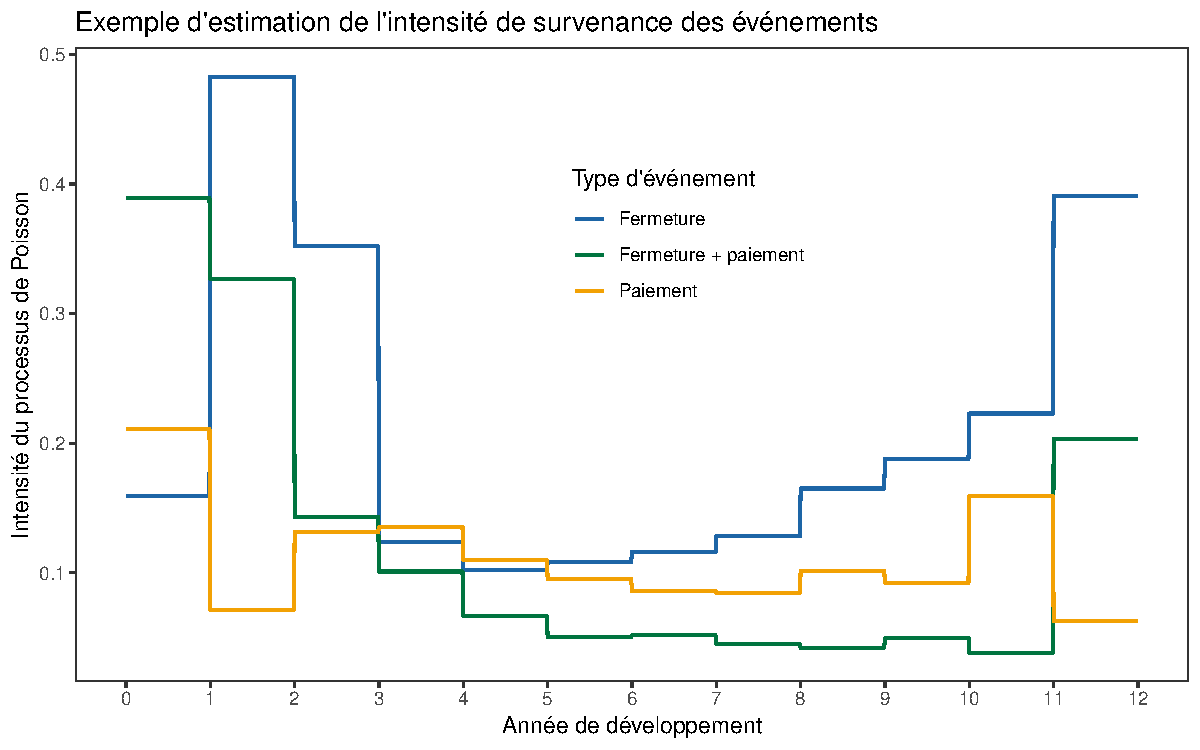
\includegraphics[width = \textwidth]{fonctions_intensite_evenements_janvier_2020.pdf}
    \end{figure}

\end{frame}

% ----------

\begin{frame}{Simulation d'une réclamation RBNS}
    
    \begin{itemize}
        \onslide<2->{\item[\circled{1}] \textbf{Simuler le temps avant le prochain événement.}}
        \onslide<4->{\item[\circled{2}] \textbf{Simuler le type d'événement.}}
        \onslide<6->{
            \item[\circled{3}] \textbf{Selon le type d'événement simulé, choisir l'action à effectuer:}
            \begin{itemize}
                \cercle \alert{Paiement}: simuler le montant du paiement, retourner à \circled{1}.
                \cercle \alert{Paiement $+$ fermeture}: simuler le montant, arrêter la simulation.
                \cercle \alert{Fermeture}: arrêter la simulation.
            \end{itemize}
        }
    \end{itemize}
    
    \begin{figure}
    	\centering
    	\begin{tikzpicture}[scale = 0.8, color = mgris]
    		
    		\onslide<1->{\draw[->, very thick] (0, 0) -- (13.5, 0);}
    		\onslide<1->{\draw[dashed, thick] (7, -1) -- (7, 3);}
    		\onslide<1->{\node at (7, -1.5) {Date};}
    		\onslide<1->{\node at (7, -2) {d'évaluation};}
    		
    		\onslide<1->{\node at (2, 2) {\croixrouge};}
    		\onslide<1->{\draw[dotted, thick] (2.2, 2) -- (6, 2);}
    		\onslide<1->{\node at (6.1, 2) {\trianglevert};}
    		\onslide<1->{\draw[line width = 0.25mm] (6.25, 2) -- (7, 2);}
    		\onslide<3-6>{\draw[line width = 0.25mm, grispale] (7, 2) -- (9.8, 2);}
    		\onslide<5->{\fill[mbleupalepale] (10, 2) circle (0.13);}
    		\onslide<7->{\draw[line width = 0.25mm, grispale] (7, 2) -- (9.6, 2);}
    		\onslide<7->{\fill[mbleupalepale] (10, 2) circle (0.3);}
    		\onslide<8->{\draw[line width = 0.25mm, grispale] (10.4, 2) -- (12, 2);}
    		\onslide<9->{\draw[fill = grispale, color = grispale](12, 1.9) rectangle ++(0.2, 0.2);}
    		
    		\onslide<10->{\node at (1, 1) {\croixrouge};}
    		\onslide<10->{\draw[dotted, thick] (1.2, 1) -- (3, 1);}
    		\onslide<10->{\node at (3.1, 1) {\trianglevert};}
    		\onslide<10->{\draw[line width = 0.25mm] (3.25, 1) -- (5, 1);}
    		\onslide<10->{\fill[mbleupale] (5.2, 1) circle (0.11);}
    		\onslide<10->{\draw[line width = 0.25mm] (5.4, 1) -- (7, 1);}
    		\onslide<11->{\draw[line width = 0.25mm, grispale] (7, 1) -- (8.55, 1);}
    		\onslide<12->{\fill[mbleupalepale] (8.7, 1) circle (0.11);}
    		\onslide<13->{\draw[line width = 0.25mm, grispale] (8.85, 1) -- (10.5, 1);}
    		\onslide<14->{\fill[grispale] (10.5, 1) circle (0.16);}
    		
    		\onslide<1->{\node[anchor = west] at (0, -0.5) {\footnotesize Accident};}
            \onslide<1->{\node[anchor = west] at (0, -0.9) {\footnotesize Déclaration};}
            \onslide<1->{\node[anchor = west] at (0, -1.3) {\footnotesize Paiement};}
            \onslide<1->{\node[anchor = west] at (0, -1.7) {\footnotesize Paiement $+$ Fermeture};}
            \onslide<1->{\node[anchor = west] at (0, -2.1) {\footnotesize Fermeture};}
            
            \onslide<1->{\node at (-0.1, -0.5) {\croixrouge};}
            \onslide<1->{\node at (-0.1, -0.9) {\trianglevert};}
            \onslide<1->{\fill[mbleupalepale] (-0.1, -1.3) circle (0.13);}
            \onslide<1->{\fill[grispale] (-0.1, -1.7) circle (0.13);}
            \onslide<1->{\draw[fill = grispale, color = grispale](-0.195, -2.2) rectangle ++(0.2, 0.2);}
    		
    	\end{tikzpicture}
    \end{figure}

\end{frame}


% ----------

\begin{frame}{Simulation d'une réclamation IBNR}

    \begin{itemize}
        \onslide<1->{\item[\circled{1}] \textbf{Simuler la survenance de la réclamation.}}
        \onslide<3->{\item[\circled{2}] \textbf{Simuler le délai de déclaration, sachant que la déclaration est postérieure à la date d'évaluation.}}
        \onslide<5->{\item[\circled{3}] \textbf{Simuler le processus de développement de la même manière qu'une réclamation RBNS.}}
    \end{itemize}
    
    
    \begin{figure}
    	\centering
    	\begin{tikzpicture}[scale = 0.8, color = mgris]
    		
    		\draw[->, very thick] (0, 0) -- (13.5, 0);
    		\draw[dashed, thick] (7, -1) -- (7, 3);
    		\node at (7, -1.5) {Date};
    		\node at (7, -2) {d'évaluation};
    		
    		\onslide<2->{\node at (5, 2) {\croixrouge};}
    		\onslide<4->{\draw[dotted, thick, grispale] (5.2, 2) -- (8.1, 2);}
    		\onslide<4->{\node at (8.2, 2) {\trianglevert};}
    		\onslide<6->{\draw[line width = 0.25mm, grispale] (8.3, 2) -- (9, 2);}
    		\onslide<6->{\fill[mbleupalepale] (9.2, 2) circle (0.17);}
    		\onslide<6->{\draw[line width = 0.25mm, grispale] (9.4, 2) -- (11, 2);}
    		\onslide<6->{\fill[mbleupalepale] (11.2, 2) circle (0.17);}
    		\onslide<6->{\draw[line width = 0.25mm, grispale] (11.4, 2) -- (12, 2);}
    		\onslide<6->{\draw[fill = grispale, color = grispale](12, 1.9) rectangle ++(0.2, 0.2);}
    		
    		\onslide<2->{\node at (3.5, 1) {\croixrouge};}
    		\onslide<4->{\draw[dotted, thick, grispale] (3.7, 1) -- (8.9, 1);}
    		\onslide<4->{\node at (9.1, 1) {\trianglevert};}
    		\onslide<6->{\draw[line width = 0.25mm, grispale] (9.25, 1) -- (11, 1);}
    		\onslide<6->{\fill[grispale] (11, 1) circle (0.19);}
    		
    		\node[anchor = west] at (0, -0.5) {\footnotesize Accident};
            \node[anchor = west] at (0, -0.9) {\footnotesize Déclaration};
            \node[anchor = west] at (0, -1.3) {\footnotesize Paiement};
            \node[anchor = west] at (0, -1.7) {\footnotesize Paiement $+$ Fermeture};
            \node[anchor = west] at (0, -2.1) {\footnotesize Fermeture};
            
            \node at (-0.1, -0.5) {\croixrouge};
            \node at (-0.1, -0.9) {\trianglevert};
            \fill[mbleupalepale] (-0.1, -1.3) circle (0.13);
            \fill[grispale] (-0.1, -1.7) circle (0.13);
            \draw[fill = grispale, color = grispale](-0.195, -2.2) rectangle ++(0.2, 0.2);
    		
    	\end{tikzpicture}
    \end{figure}
    
\end{frame}

% ----------

\begin{frame}{Détermination de la réserve}
    
    \begin{itemize}
        \fleche \textbf{RBNS}
            \begin{itemize}
                \cercle Simuler le processus de développement de toutes les réclamations RBNS du portefeuille.
            \end{itemize}
        
        \fleche \textbf{IBNR}
            \begin{itemize}
                \cercle Simuler la survenance des réclamations IBNR.
                \cercle Simuler le délai de déclaration des réclamations IBNR.
                \cercle Simuler le processus de développement des réclamations IBNR.
            \end{itemize}
        \fleche \textbf{Réserve simulée = somme des paiements simulés}
        \fleche \textbf{Plusieurs simulations pour obtenir la distribution prédictive.}
    \end{itemize}
    
    \begin{alertblock}{Note}
        Pour les réclamations IBNR, il faut simuler les variables explicatives puisqu'elles ne sont pas observées à la date d'évaluation.
    \end{alertblock}
    
\end{frame}

% ----------

\section{Adaptation aux données simulées}

% ----------

\begin{frame}{Simulation des données de réclamations}

    \begin{itemize}[itemsep = 0.4cm]
        \fleche Données simulées avec \texttt{Gabrielli, A., \& Wüthrich, M. (2018). An individual claims history simulation machine. \emph{Risks, 6}(2).}
        \fleche Plusieurs réseaux de neurones entrainés sur des données réelles.
        \fleche Le délai de déclaration et le processus de développement dépendent de 6 caractéristiques de la réclamation (\texttt{ligne d'affaire}, \texttt{code de réclamation}, \texttt{année d'accident}, \texttt{trimestre d'accident}, \texttt{âge}, \texttt{partie du corps blessée}).
        \fleche Simulation en temps discret.
    \end{itemize}
    
\end{frame}

% ----------

\begin{frame}{Simulation des données de réclamations (suite)}

    \textbf{Extrait de la base de données simulée}:

    \resizebox{\textwidth}{!}{
    \begin{table}[h]
        \centering
        \begin{tabular}{c|cccccc|c|ccccc|ccccc}
            \toprule
            \midrule
            \textbf{Claim #} & \textbf{LoB} & \textbf{cc} & \textbf{AY} & \textbf{AQ} & \textbf{age} & \textbf{inj\_part} & \textbf{RepDel} & \textbf{Pay00} & \textbf{Pay01} & \textbf{Pay02} & \textbf{\dots} & \textbf{Pay11} & \textbf{Open00} & \textbf{Open01} & \textbf{Open02} & \textbf{\dots} & \textbf{Open11}\\
            \midrule
            \rowcolor{gray!15} 1 & 3 & 17 & 94 & 2 & 23 & 11 & 0 & 0 & 0 & 0 & \dots & 0 & 0 & 0 & 0 & \dots & 0\\
            2 & 4 & 19 & 94 & 3 & 32 & 21 & 0 & 113 & 0 & 0 & \dots & 0 & 1 & 0 & 0 & \dots & 0\\
            \rowcolor{gray!15} 3 & 4 & 39 & 94 & 2 & 47 & 10 & 0 & 180 & 0 & 0 & \dots & 0 & 0 & 0 & 0 & \dots & 0\\
            4 & 3 & 27 & 94 & 4 & 35 & 51 & 0 & 0 & 2582 & 0 & \dots & 0 & 1 & 0 & 0 & \dots & 0\\
            \rowcolor{gray!15} 5 & 2 & 29 & 94 & 1 & 15 & 61 & 0 & 0 & 1656 & 0 & \dots & 0 & 1 & 0 & 0 & \dots & 0\\
            6 & 2 & 9 & 94 & 2 & 63 & 53 & 0 & 3094 & 0 & 0 & \dots & 0 & 0 & 0 & 0 & \dots & 0\\
            \rowcolor{gray!15} 7 & 4 & 42 & 94 & 1 & 41 & 21 & 0 & 631 & 0 & 0 & \dots & 0 & 0 & 0 & 0 & \dots & 0\\
            8 & 2 & 43 & 94 & 3 & 35 & 52 & 0 & 0 & 2059 & 0 & \dots & 0 & 1 & 0 & 0 & \dots & 0\\
            \rowcolor{gray!15} 9 & 2 & 34 & 94 & 1 & 45 & 10 & 0 & 0 & 0 & 0 & \dots & 0 & 0 & 0 & 0 & \dots & 0\\
            10 & 2 & 1 & 94 & 4 & 37 & 34 & 0 & 0 & 1039 & 0 & \dots & 0 & 1 & 0 & 0 & \dots & 0\\
            \hline
            \bottomrule
        \end{tabular}
    \end{table}
    }

\end{frame}

% ----------

\begin{frame}{Adaptation du modèle aux données simulées}

    \begin{itemize}
        \fleche \textbf{Modifications faites au modèle}
        \begin{itemize}
            \cercle On peut voir les données discrètes comme des données continues qui, miraculeusement, ressemblent à des données discrètes.
            \cercle Seul problème: le délai de déclaration, modélisé par une loi Weibull.
            \cercle On remplace donc la Weibull par n'importe quelle loi discrète (j'ai utilisé une binomiale négative).
            \cercle Le modèle est entrainé sur des données discrètes, mais simule des données continues.
        \end{itemize}
        \vspace{0.5cm}
        \fleche \textbf{Modifications faites à la base de données simulée}
        \begin{itemize}
            \cercle Suppression des paiements négatifs.
            \cercle Ignorance des réouvertures.
            \cercle Autres modifications mineures.
        \end{itemize}

    \end{itemize}
    
\end{frame}

% ----------

\begin{frame}{Résultats sur données simulées}

    \begin{figure}
        \centering
        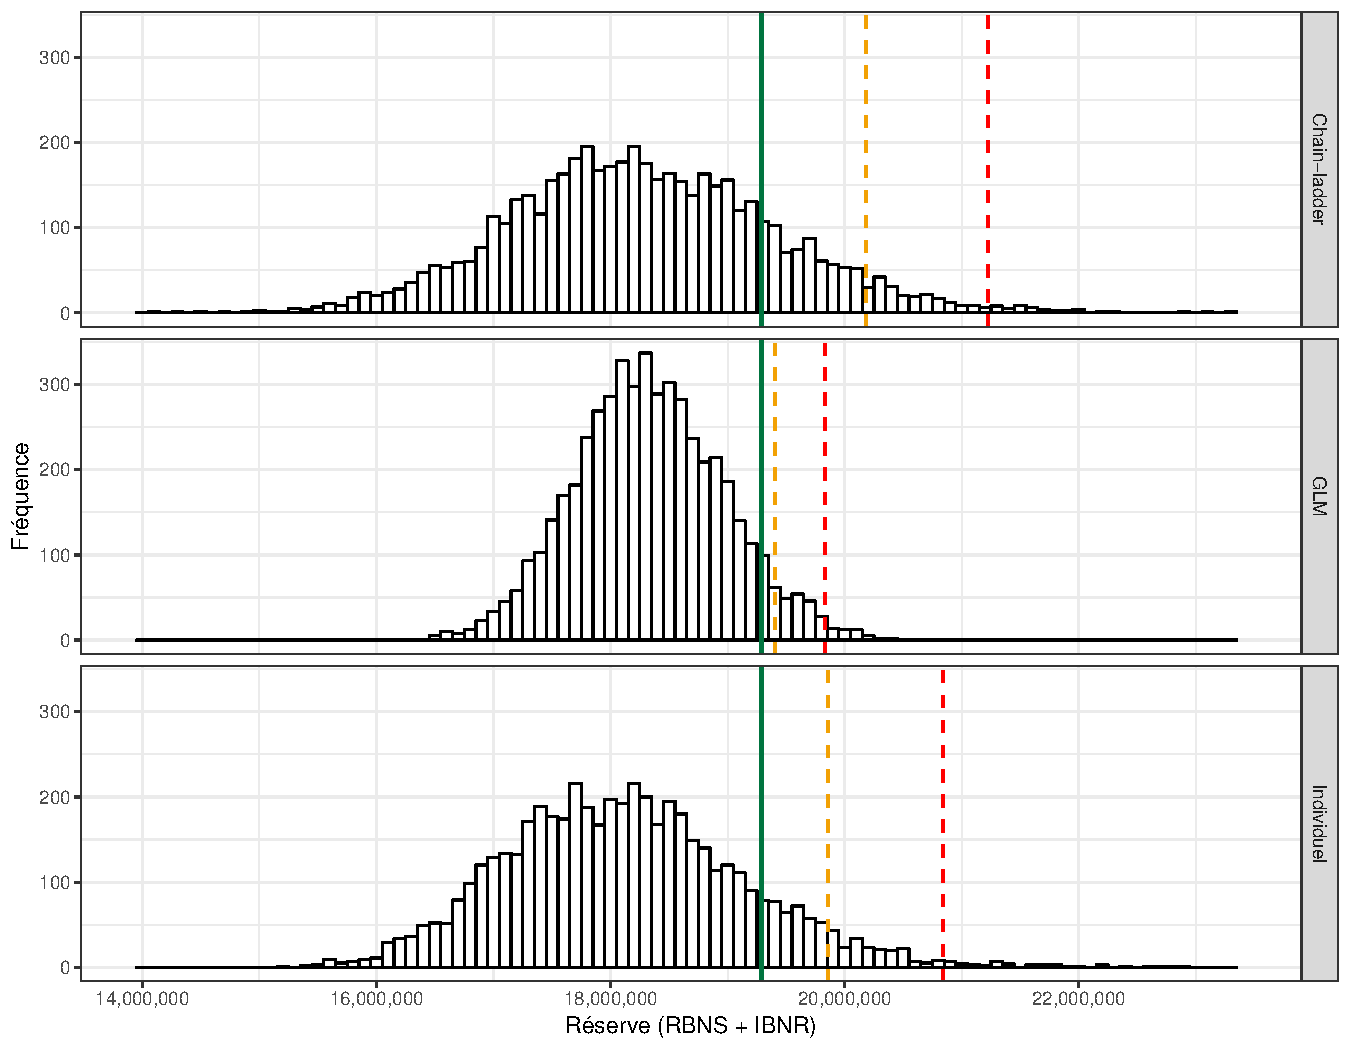
\includegraphics[width = 0.85\textwidth]{comparaison_ind_coll_2.pdf}
    \end{figure}

\end{frame}

% ----------

\section{Modifications -- Francis}

% ----------

\begin{frame}{Mise en contexte}

    \begin{exampleblock}{Question guide}
        La régression quantile permet-elle de mieux modéliser la sévérité des paiements que les GLM en provisionnement non-vie?
    \end{exampleblock}
    
    \begin{alertblock}{Résumé du projet}
        Modélisation de la sévérité des paiements avec la régression quantile. Comparaison de la performance avec un GLM (gaussien). 
    \end{alertblock}
    
    \begin{itemize}
        \fleche Ensemble d'entrainement: tous les paiements observés avant 2006.
        \fleche Ensemble de validation: tous les paiements associés au réclamations RBNS observés après 2006.
    \end{itemize}
    
    \begin{tikzpicture}[scale = 0.7, rotLabel/.style = {above = 3pt, rotate = 90, anchor = 200, right = 3pt}]
    	% Fleche ligne du temps
    	\draw[->, very thick] (0, 0) -- (15, 0);
    	% Années
    	\draw (1, 0) node[below = 3pt] {1994};
    	\draw (8, 0) node[below = 3pt] {2006};
    	% Ticks
    	\foreach \x in {1, 8}
          	\draw (\x cm,3pt) -- (\x cm, -3pt);
    	% Curly braces
    	\draw [thick, decorate, decoration = {brace, amplitude = 5pt, raise = 4pt}] (1.05, 0) -- (7.95, 0);
    	\draw [thick, decorate, decoration = {brace, amplitude = 5pt, raise = 4pt}] (8.05, 0) -- (14.7, 0);
    	% Écriture
    	\draw (4.5, 0) node[above = 10pt] {Entrainement};
    	\draw (11.35, 0) node[above = 10pt] {Validation};
    \end{tikzpicture}

\end{frame}

% ----------

\begin{frame}{Régression quantile vs régression linéaire}
    
    \begin{tcolorbox}[enhanced, notitle, clip upper, fontupper = \sffamily, tabularx = {>{\cellcolor[gray]{.5}\color{white}}r > {\centering\arraybackslash}X > {\centering\arraybackslash}X}]
    
        &\cellcolor{black!80}\color{white} \textbf{Régression linéaire} &\cellcolor{black!80}\color{white} \textbf{Régression quantile}\\
        \rowcolor{white} \textbf{Formule} & $\mathbb{E}(Y|\boldsymbol{X})= \boldsymbol{X}\boldsymbol{\beta}$ & $Q_{Y|\boldsymbol{X}}(\tau)= \boldsymbol{X}\boldsymbol{\beta}_\tau$\\
         \rowcolor{black!30} \textbf{Fonction de perte} & x^2 &$\rho_\tau(x)$\\
        \rowcolor{white} \textbf{Estimation} & \footnotesize $\widehat{\boldsymbol{\beta}} = \argmin{\beta} \frac{1}{n} \sum\limits_{i = 1}^n (y_i - \boldsymbol{x}_i\boldsymbol{\beta})^2$ & \footnotesize $\widehat{\boldsymbol{\beta}}_\tau = \argmin{\beta} \frac{1}{n} \sum\limits_{i = 1}^n \rho_\tau(y_i - \boldsymbol{x}_i\boldsymbol{\beta})$\\
        \rowcolor{black!30} \textbf{Distribution des $Y_i$} & N(\boldsymbol{x}_i\boldsymbol{\beta}, \sigma^2) & Non paramétrique \\
    \end{tcolorbox}
    
    \begin{itemize}
        \fleche Dans la régression quantile, on modélise le \textbf{quantile conditionnel} de niveau $\tau$.
        \fleche Fonction de perte:
            \begin{align*}
                \rho_\tau(x) &=
                \begin{dcases}
                    (1 - \tau)|x| & x \le 0\\
                    \tau x & x > 0
                \end{dcases} 
            \end{align*}
    \end{itemize}
    
\end{frame}

% ----------

\begin{frame}{Exemples de fonctions de perte}
    
    \begin{figure}
        \centering
        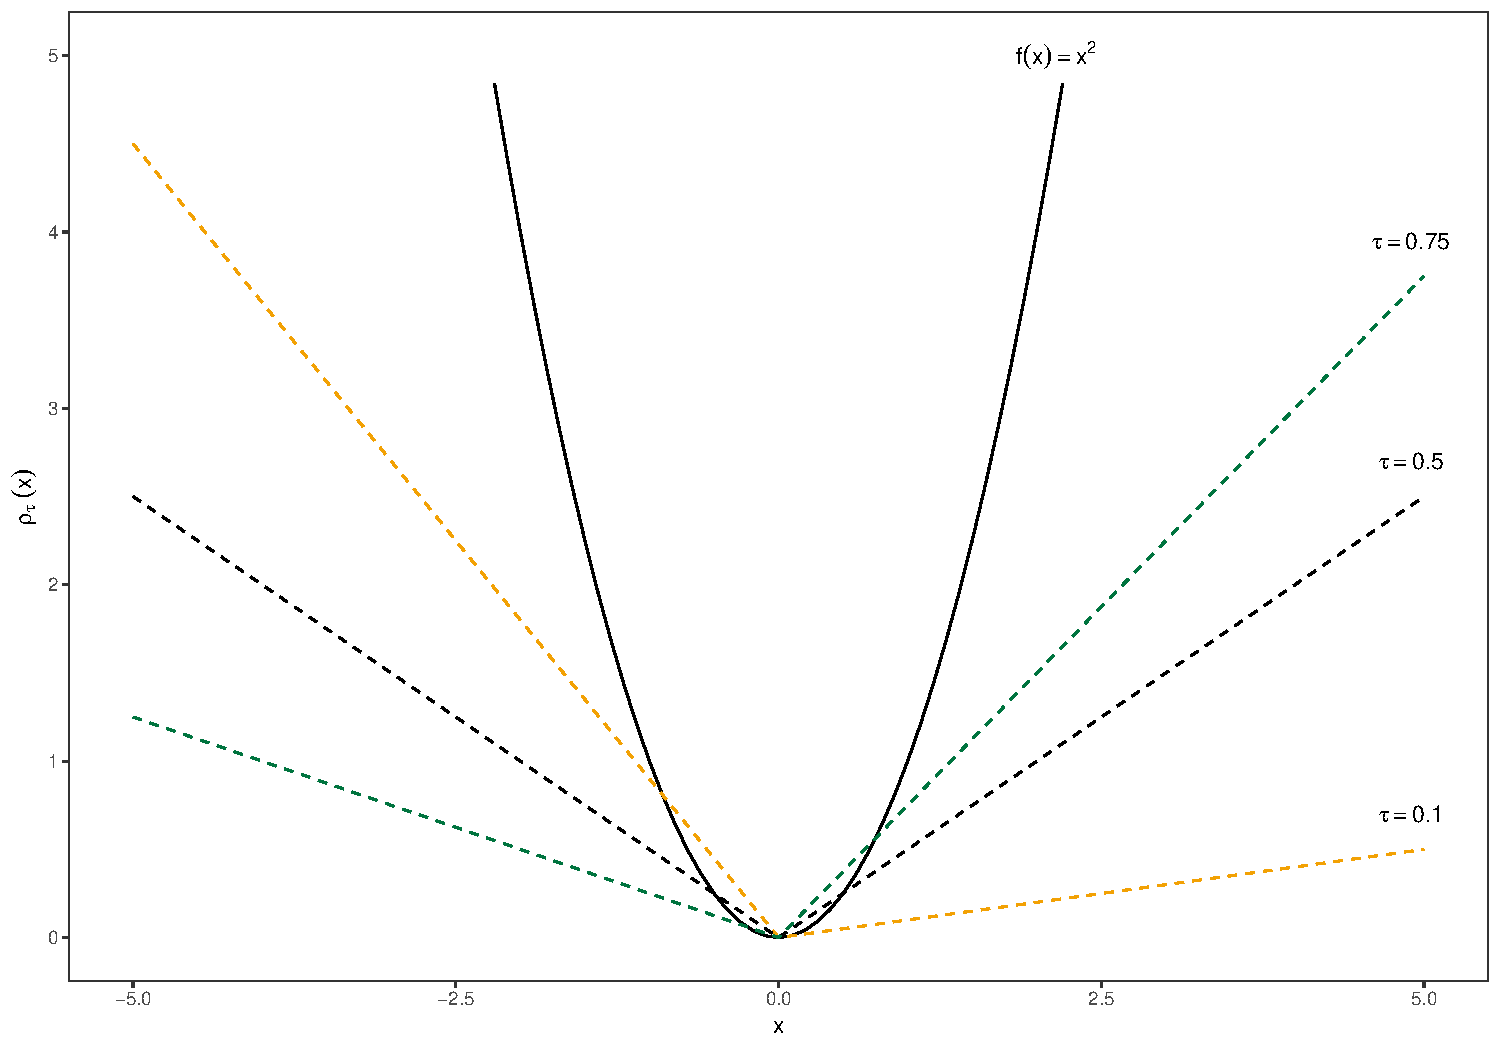
\includegraphics[width = 0.8\textwidth]{loss_functions.pdf}
    \end{figure}
    
    \begin{itemize}
        \fleche Notez que la régression quantile pénalise moins les grandes déviations que la régression linéaire, ce qui la rend plus robuste.
    \end{itemize}
    
\end{frame}

% ----------

\begin{frame}{Exemple d'ajustement -- Régression quantile}

    \begin{figure}
        \centering
        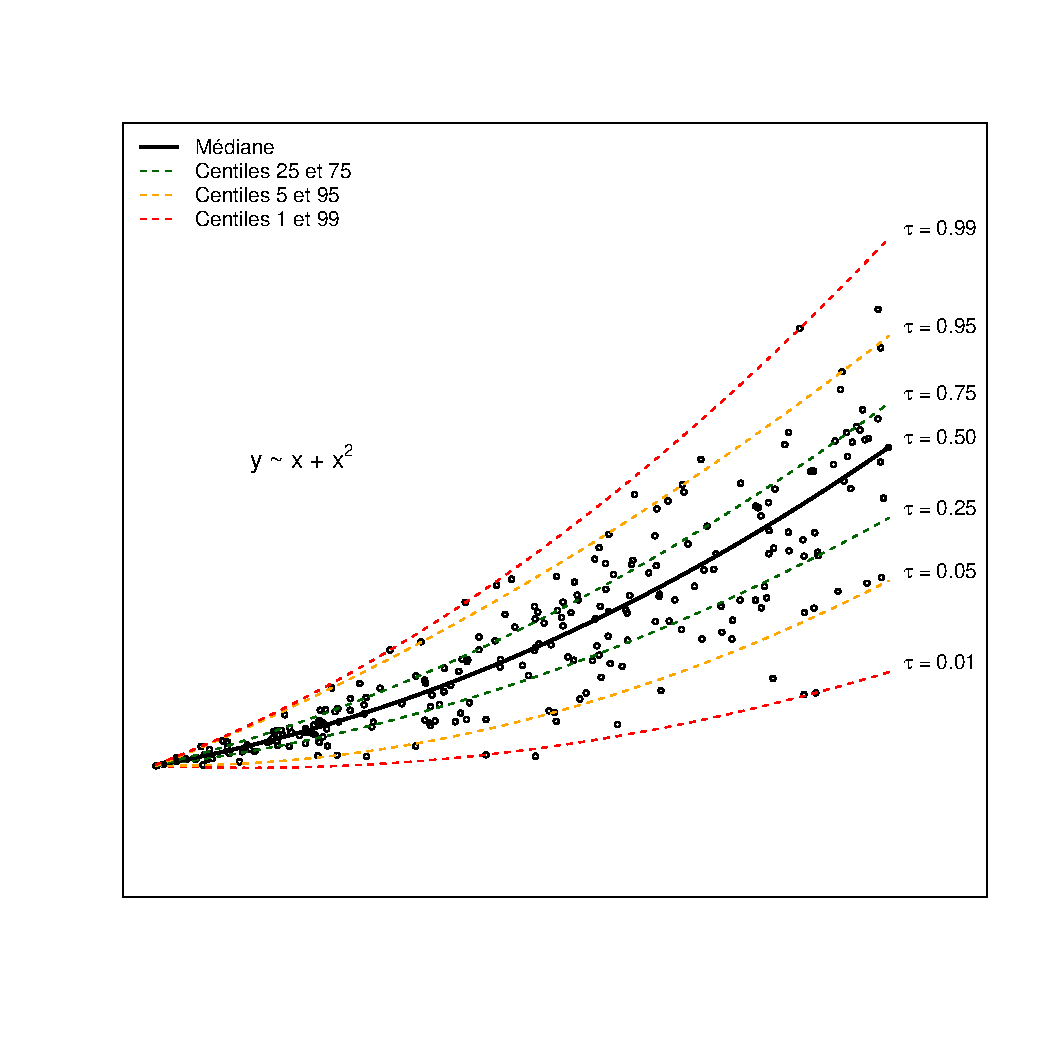
\includegraphics[width = 0.88\textwidth, trim = 0 0 0 60]{exemple_fit_rq.pdf}
    \end{figure}
    
\end{frame}

% ----------


\begin{frame}{Exemple d'ajustement -- Régression linéaire}

    \begin{figure}
        \centering
        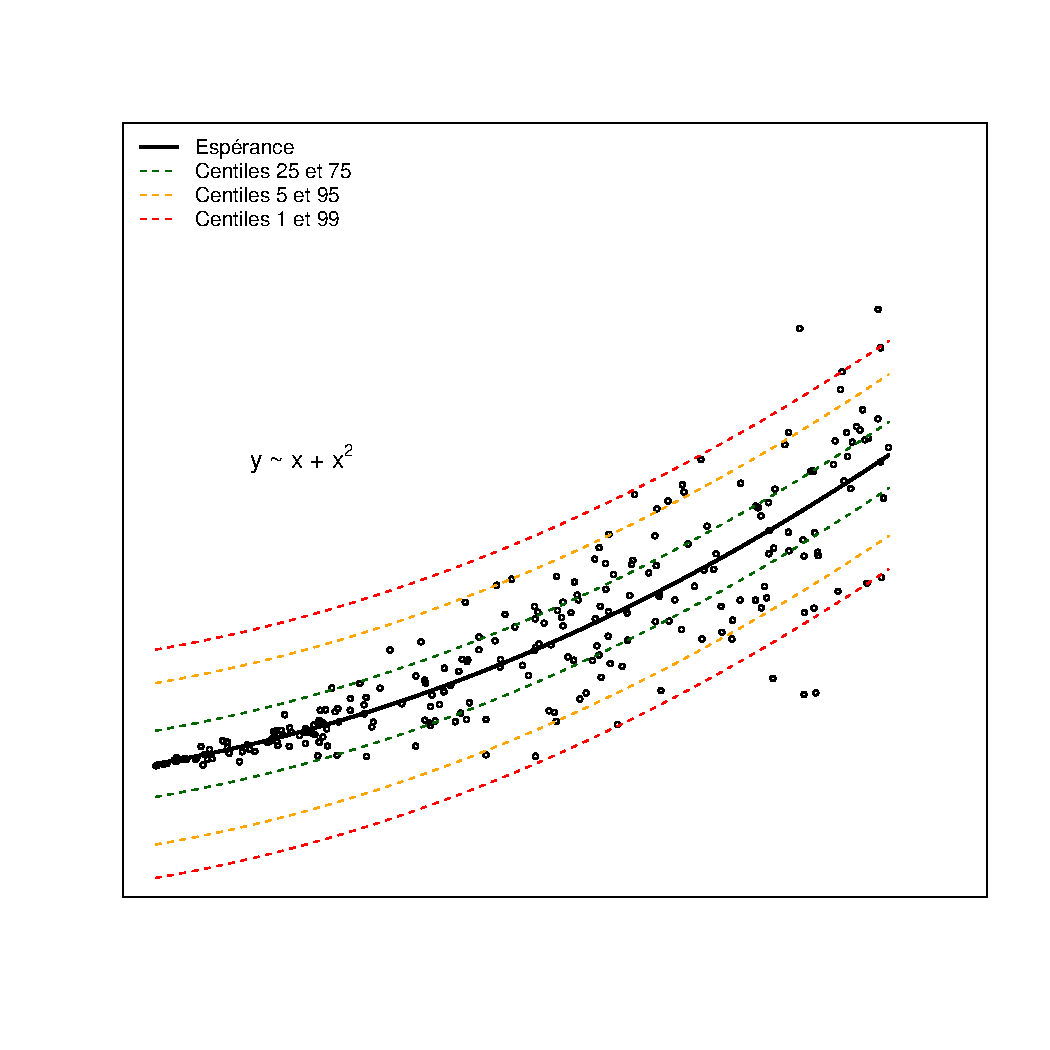
\includegraphics[width = 0.88\textwidth, trim = 0 0 0 60]{exemple_fit_lm.pdf}
    \end{figure}    

\end{frame}

% ----------

\begin{frame}{Analyse comparative}

    \begin{itemize}[itemsep = 0.4cm]
        \fleche Comparaison de la performance entre la \textbf{régression linéaire} et la \textbf{régression quantile} sur le jeu de données simulé.
        \fleche Performance mesurée avec la statistique de \textbf{Kolmogorov-Smirnov} et avec l'\textbf{erreur absolue moyenne} sur le total des paiements.
        \fleche 3 formules considérées: 
        \begin{itemize}
            \cercle Modèle catégoriel: \texttt{Log-paiement $\sim$ as.factor(DY)}
            \cercle Modèle linéaire: \texttt{Log-paiement $\sim$ DY}
            \cercle Modèle quadratique: \texttt{Log-paiement $\sim$ DY + DY$^2$}
            % \cercle Modèle cubique: \texttt{Log-paiement $\sim$ DY + DY$^2$ + DY$^3$}
        \end{itemize}
    \end{itemize}
    
\end{frame}

% ----------

\begin{frame}{Données d'entrainement et de validation}

    \begin{figure}
        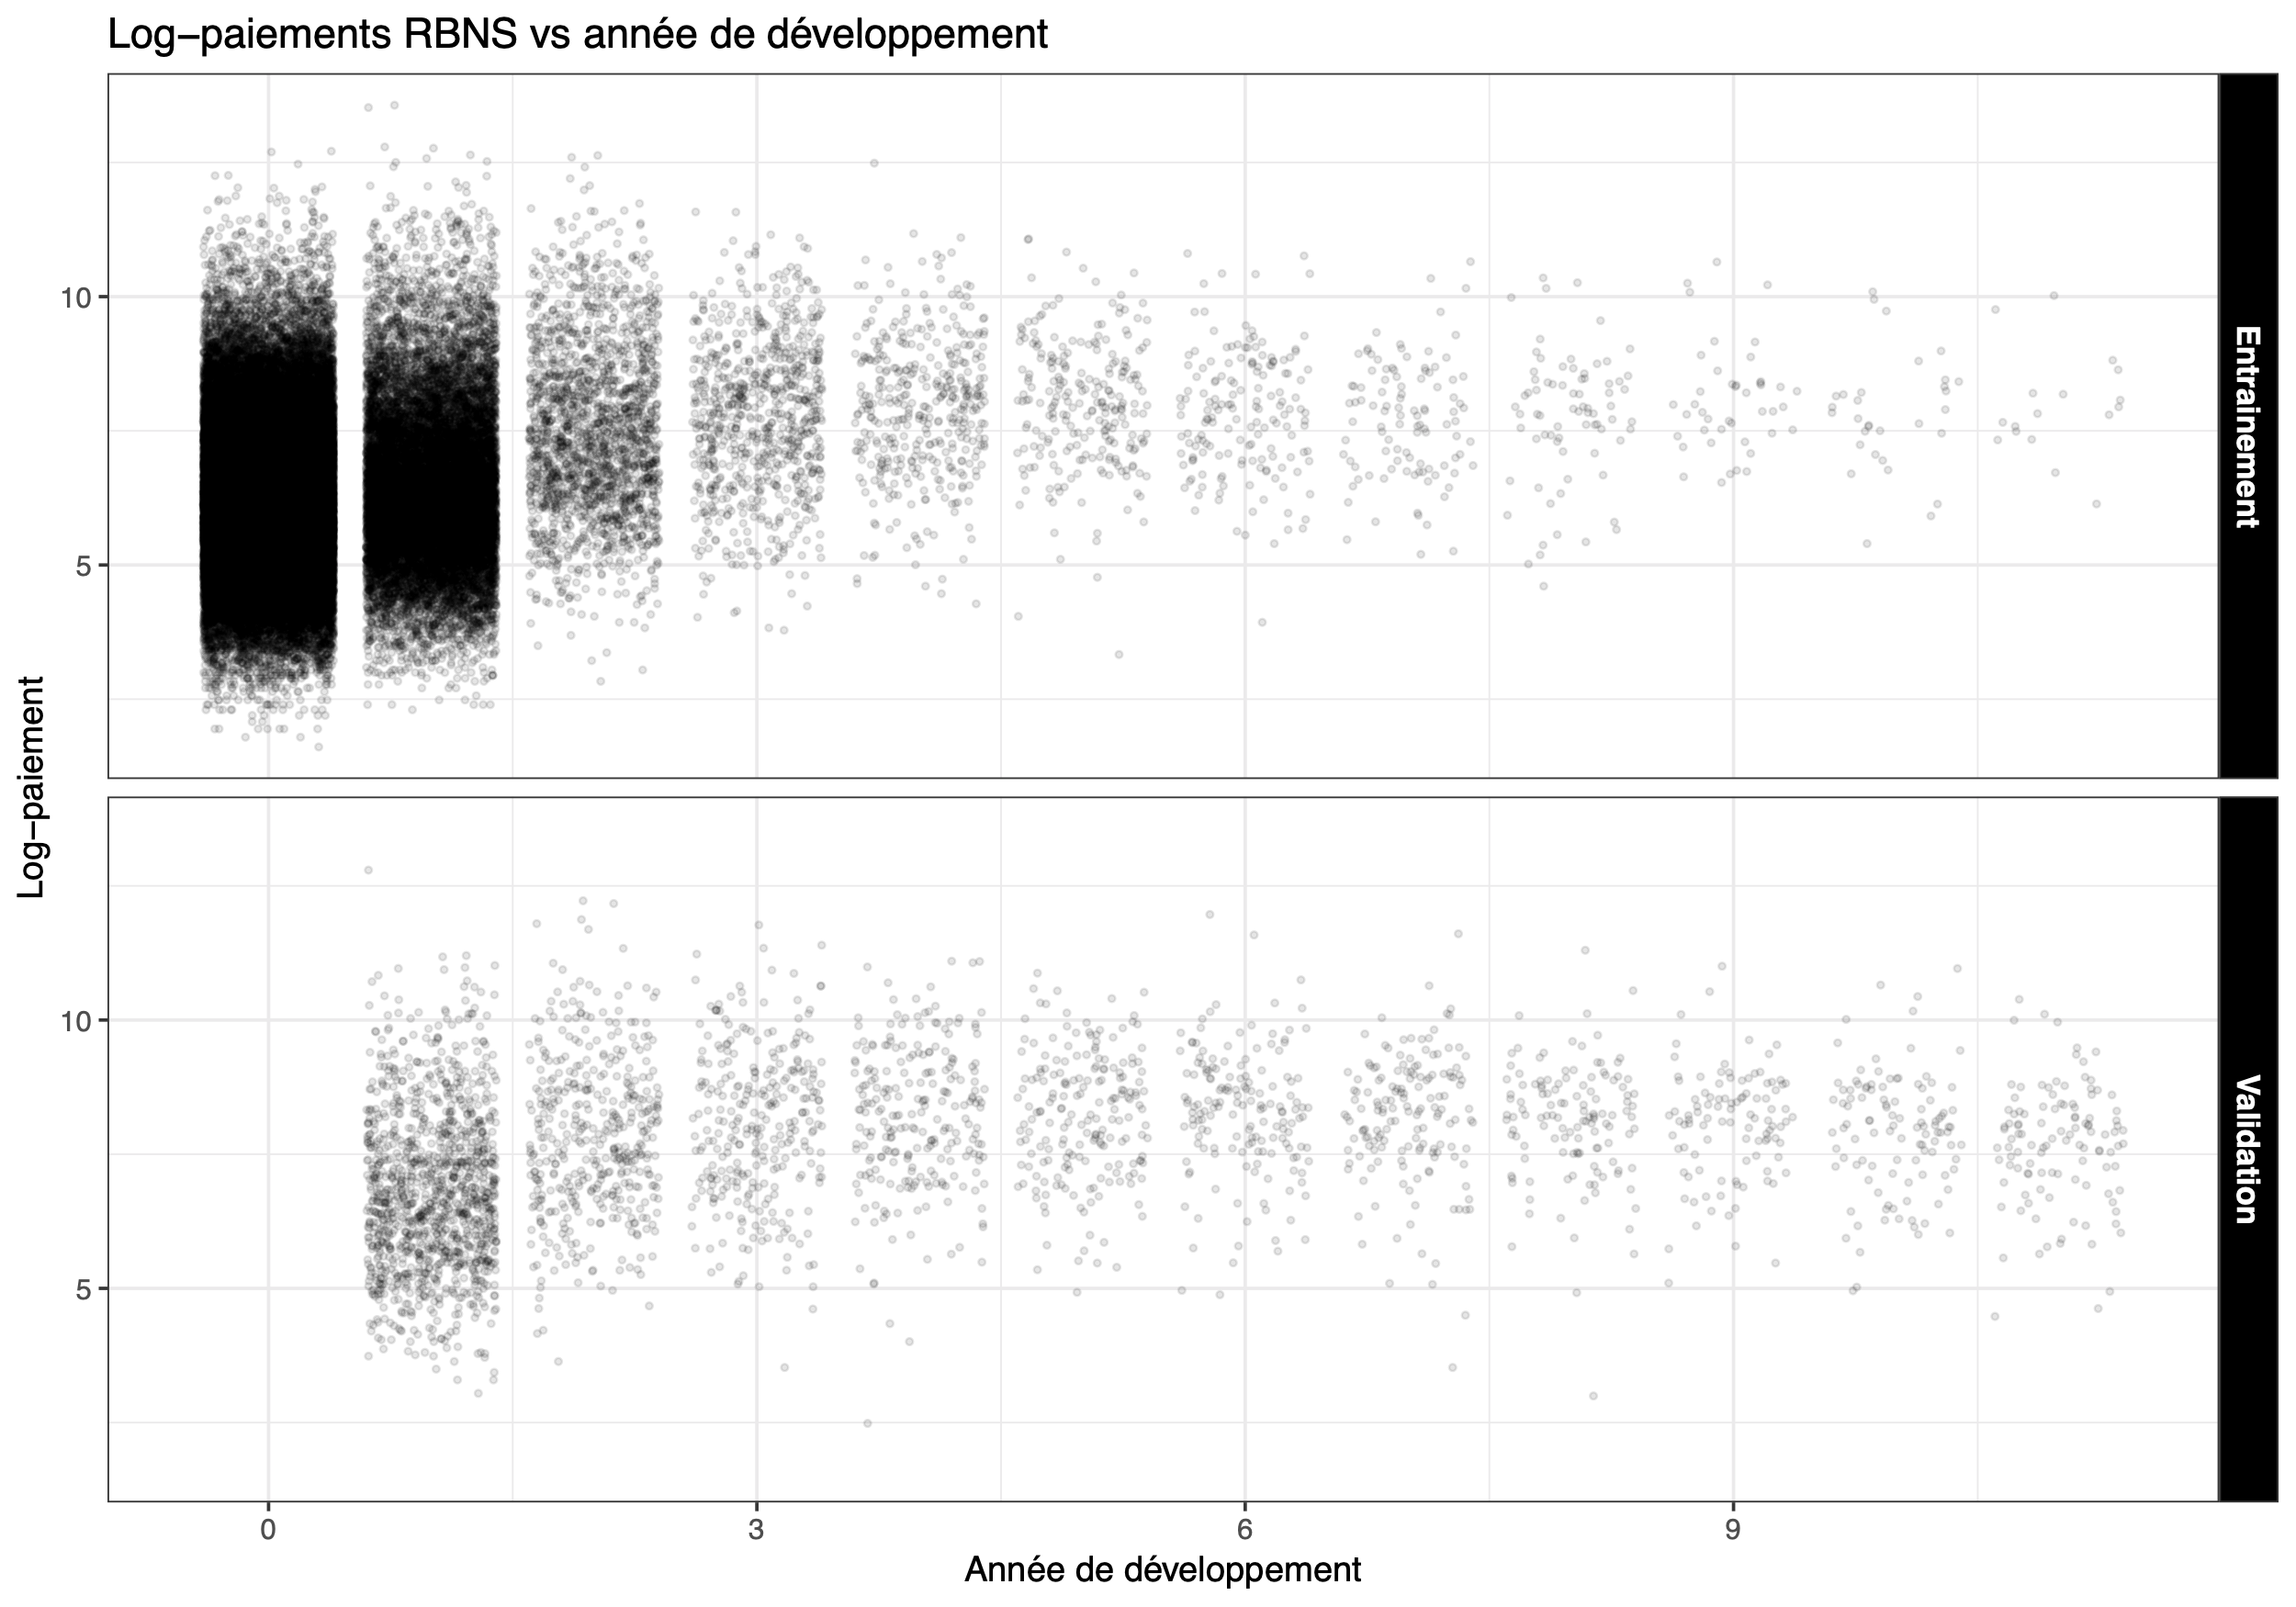
\includegraphics[width = 0.95\textwidth]{nuage_points_overleaf.png}
    \end{figure}
    
\end{frame}

% ----------

\begin{frame}{Entrainement des modèles catégoriels}
    
    \begin{figure}
        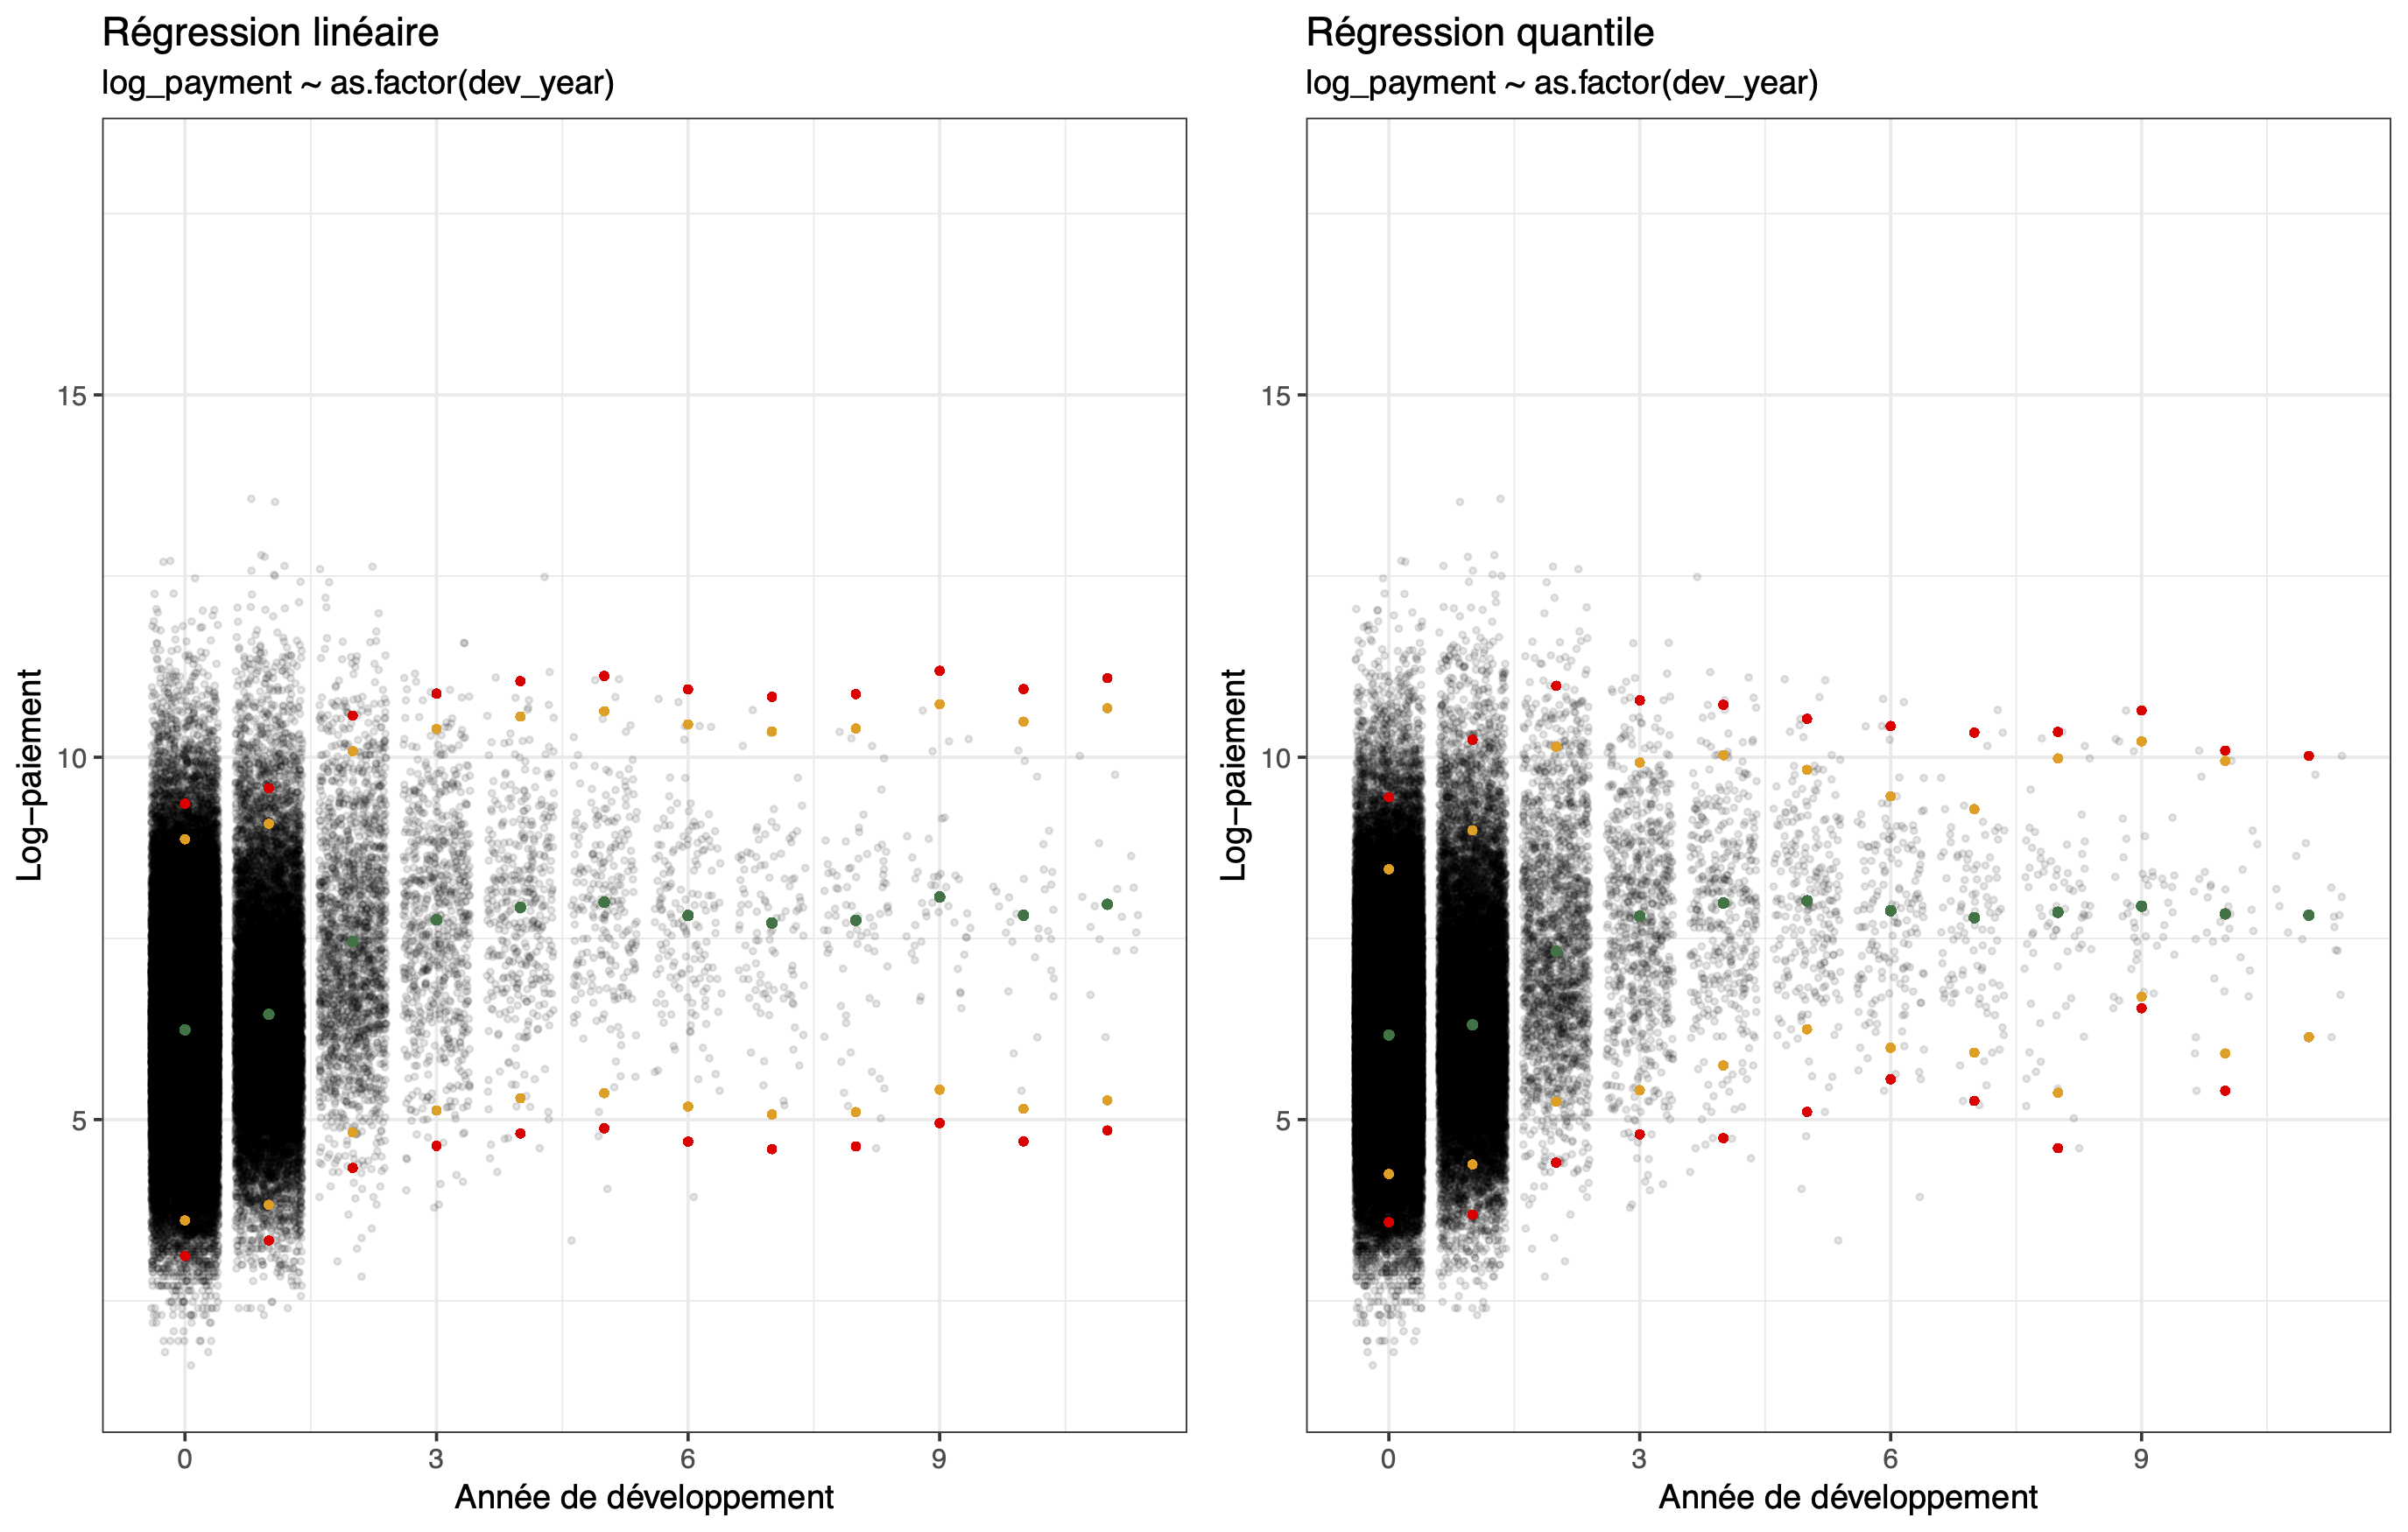
\includegraphics[width = \textwidth]{fit_fac.png}
    \end{figure}
    
\end{frame}

% ----------

\begin{frame}{Entrainement des modèles linéaires}

    \begin{figure}
        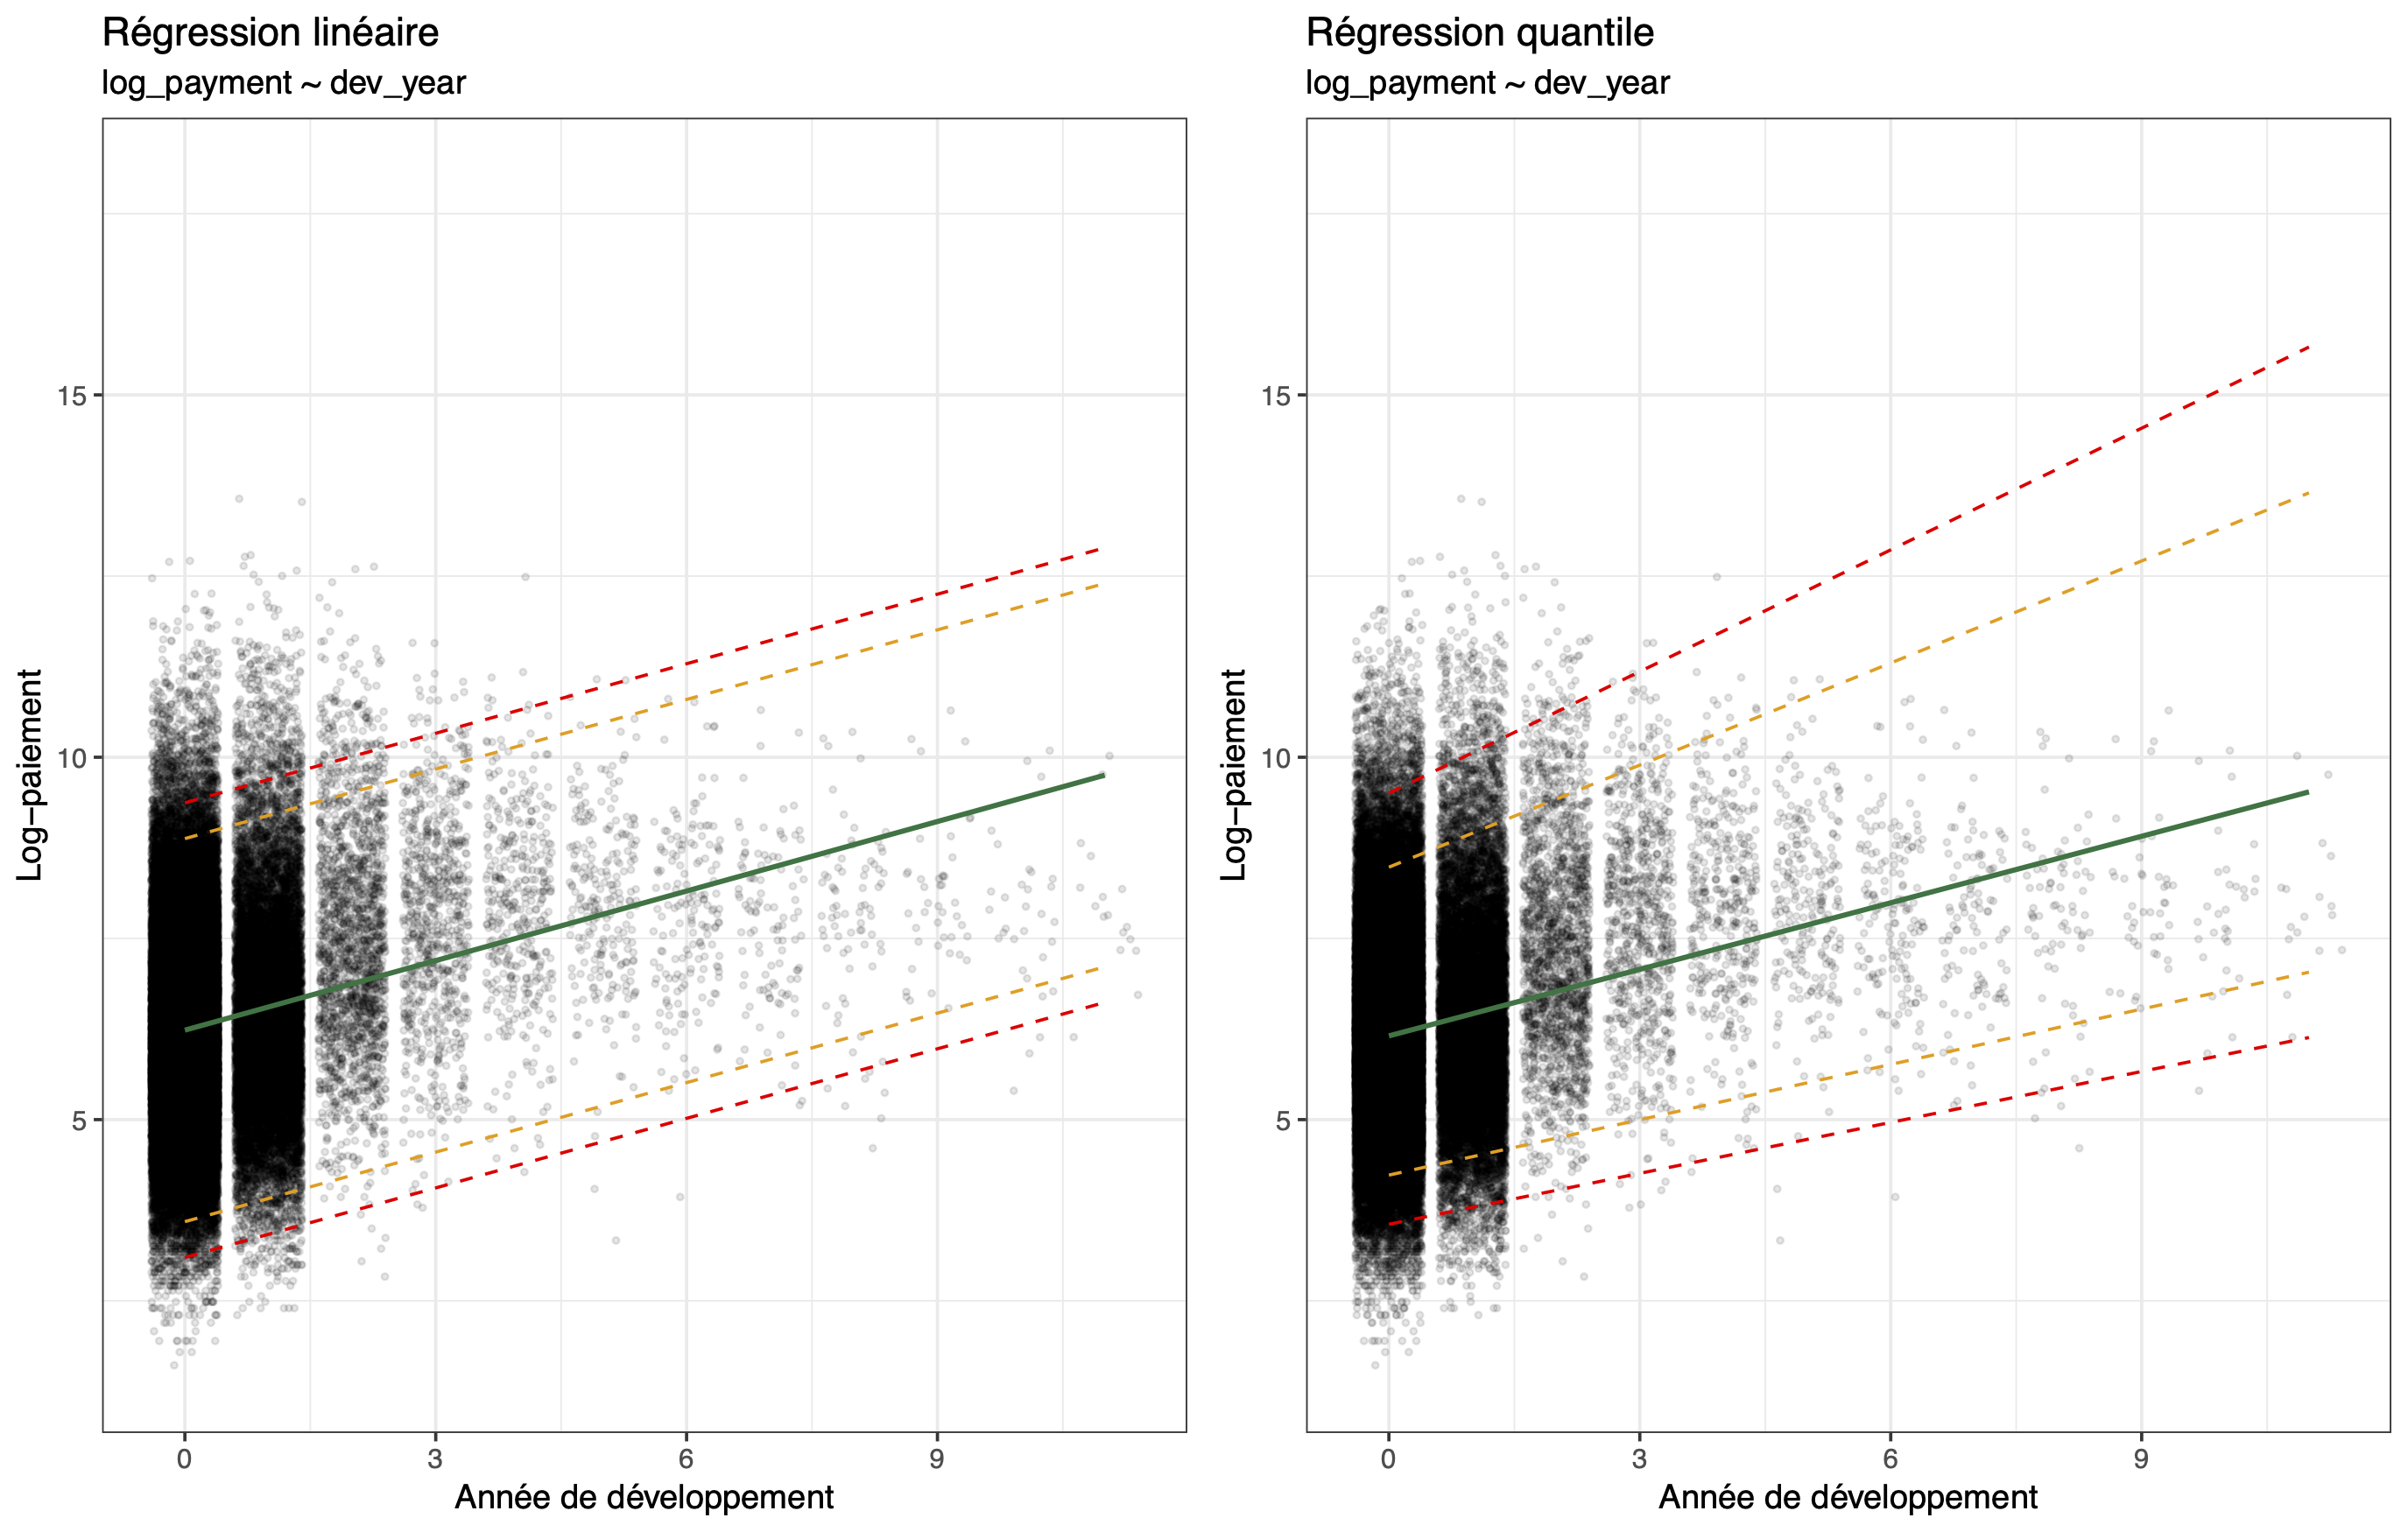
\includegraphics[width = \textwidth]{fit_degre_1.png}
    \end{figure}
    
\end{frame}

% ----------

\begin{frame}{Entrainement des modèles quadratiques}

    \begin{figure}
        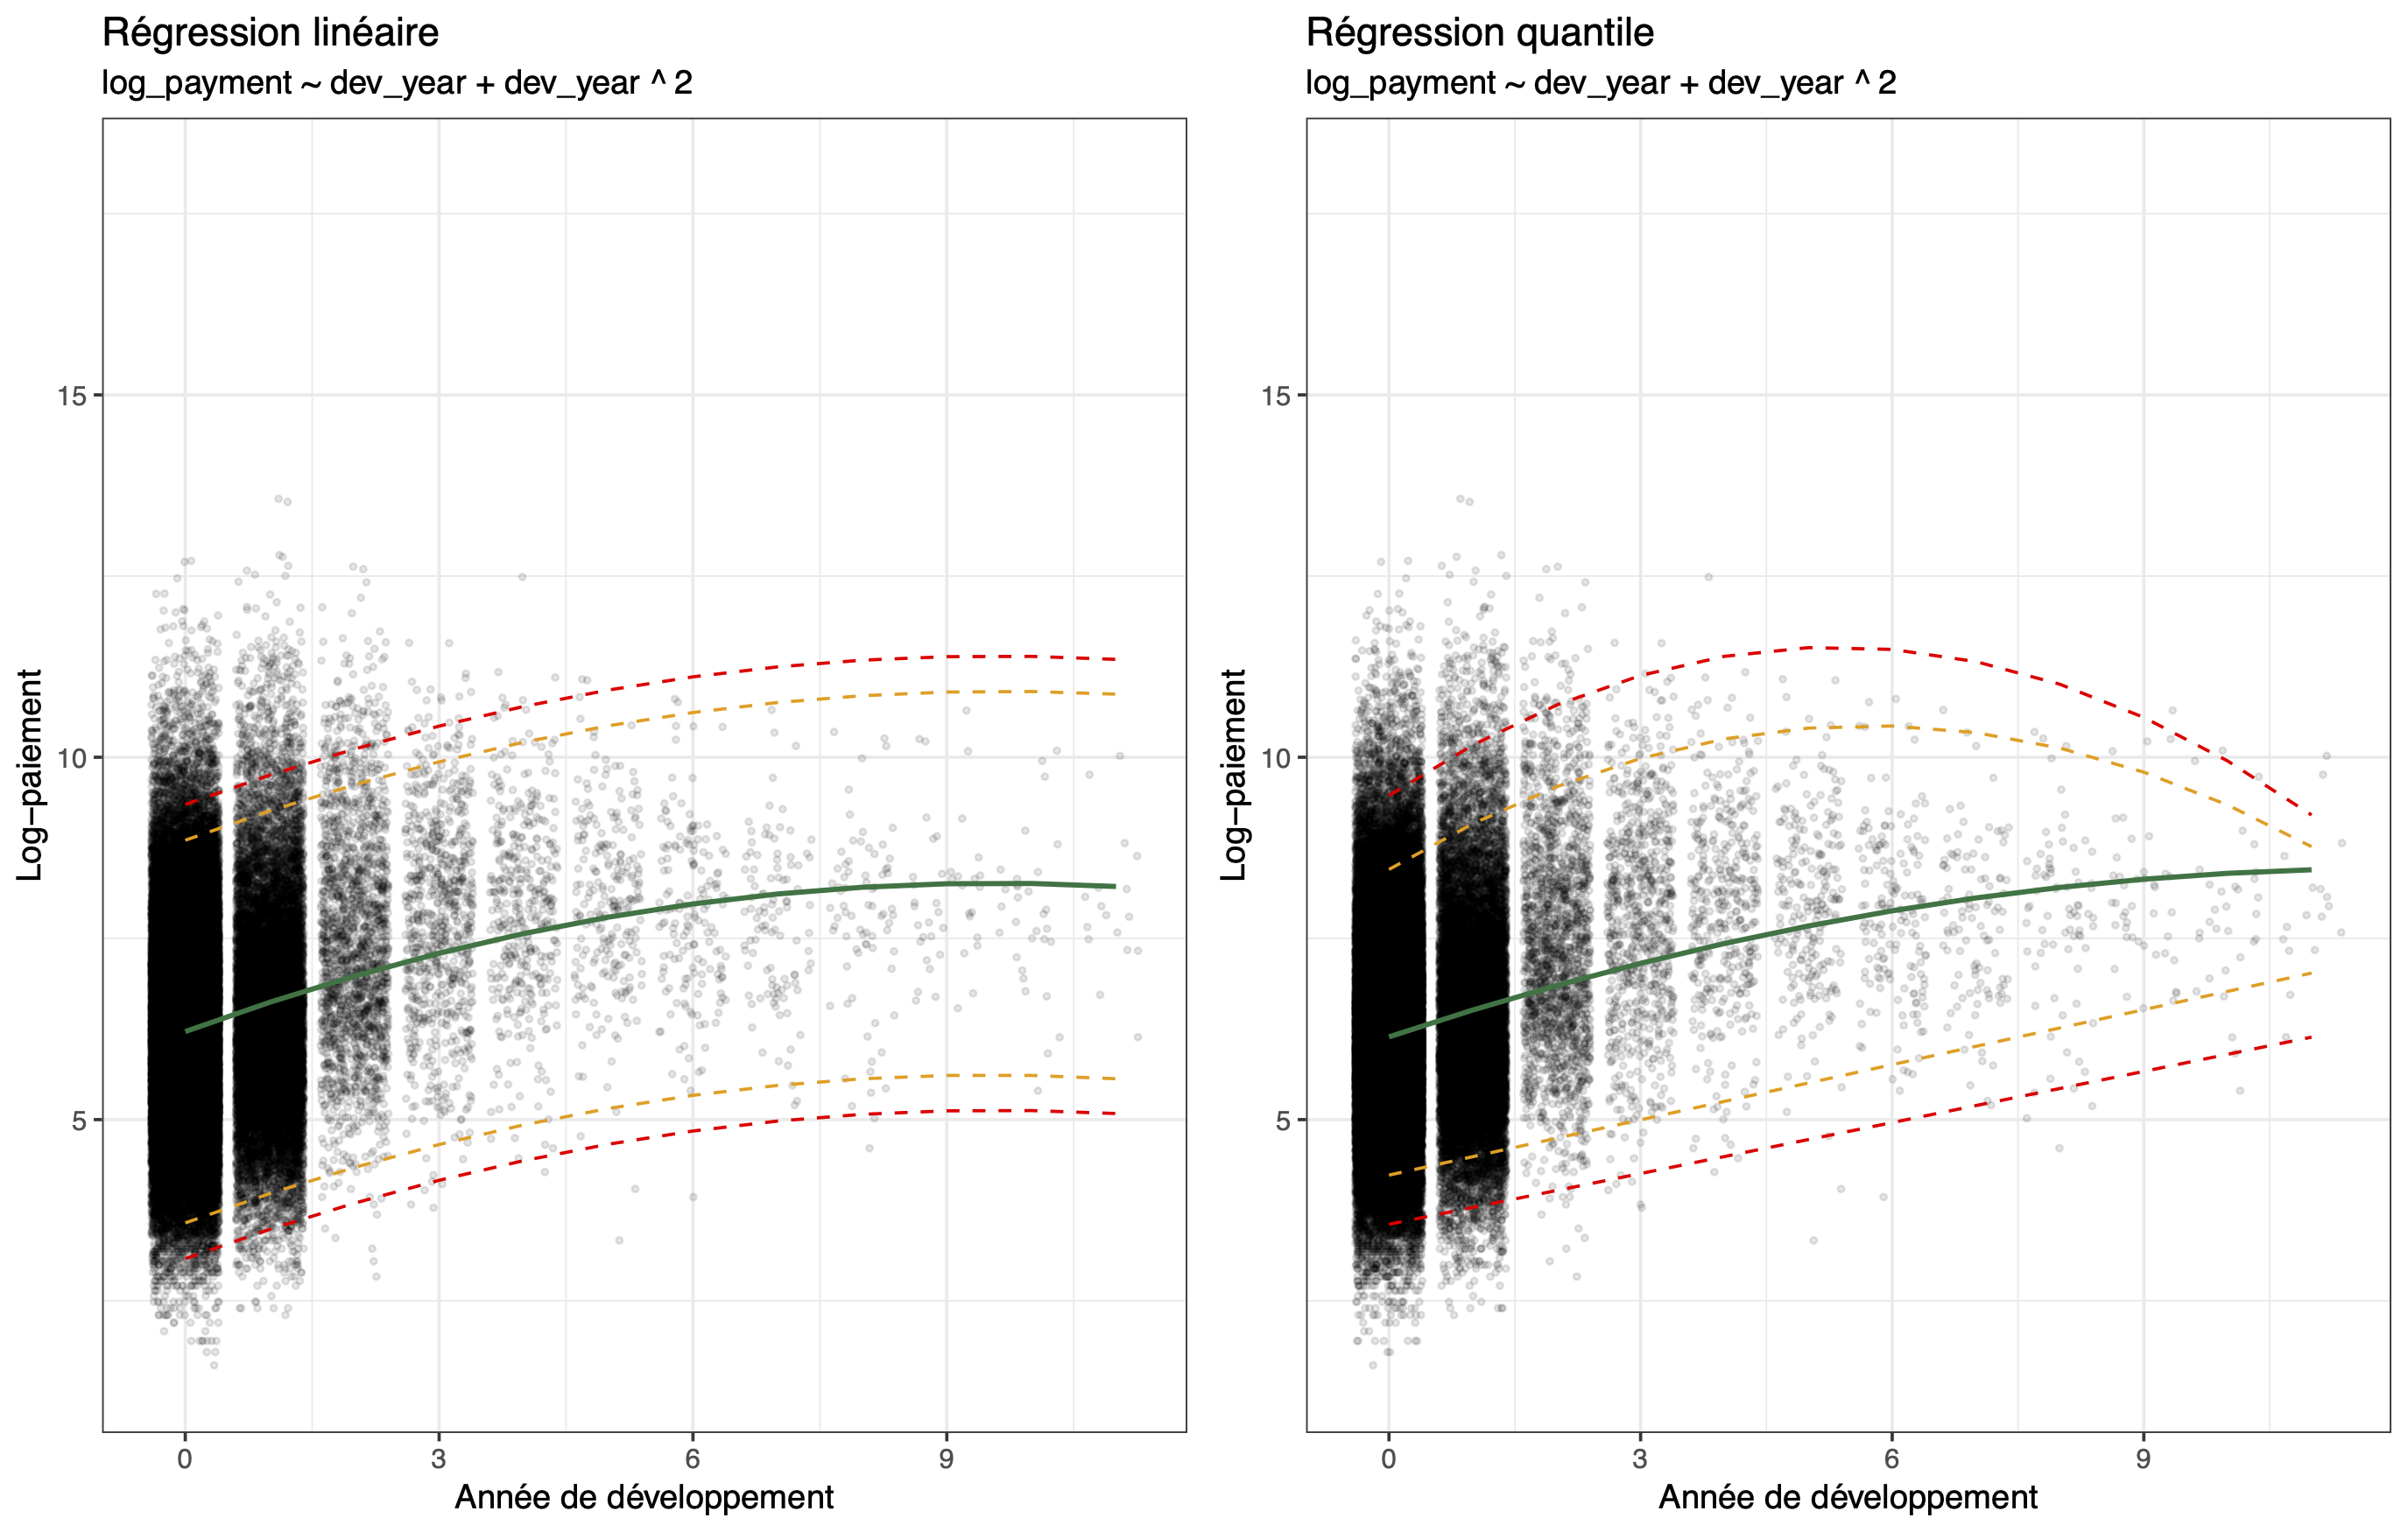
\includegraphics[width = \textwidth]{fit_degre_2.png}
    \end{figure}
    
\end{frame}

% ----------

% \begin{frame}{Entrainement des modèles cubiques}

%     \begin{figure}
%         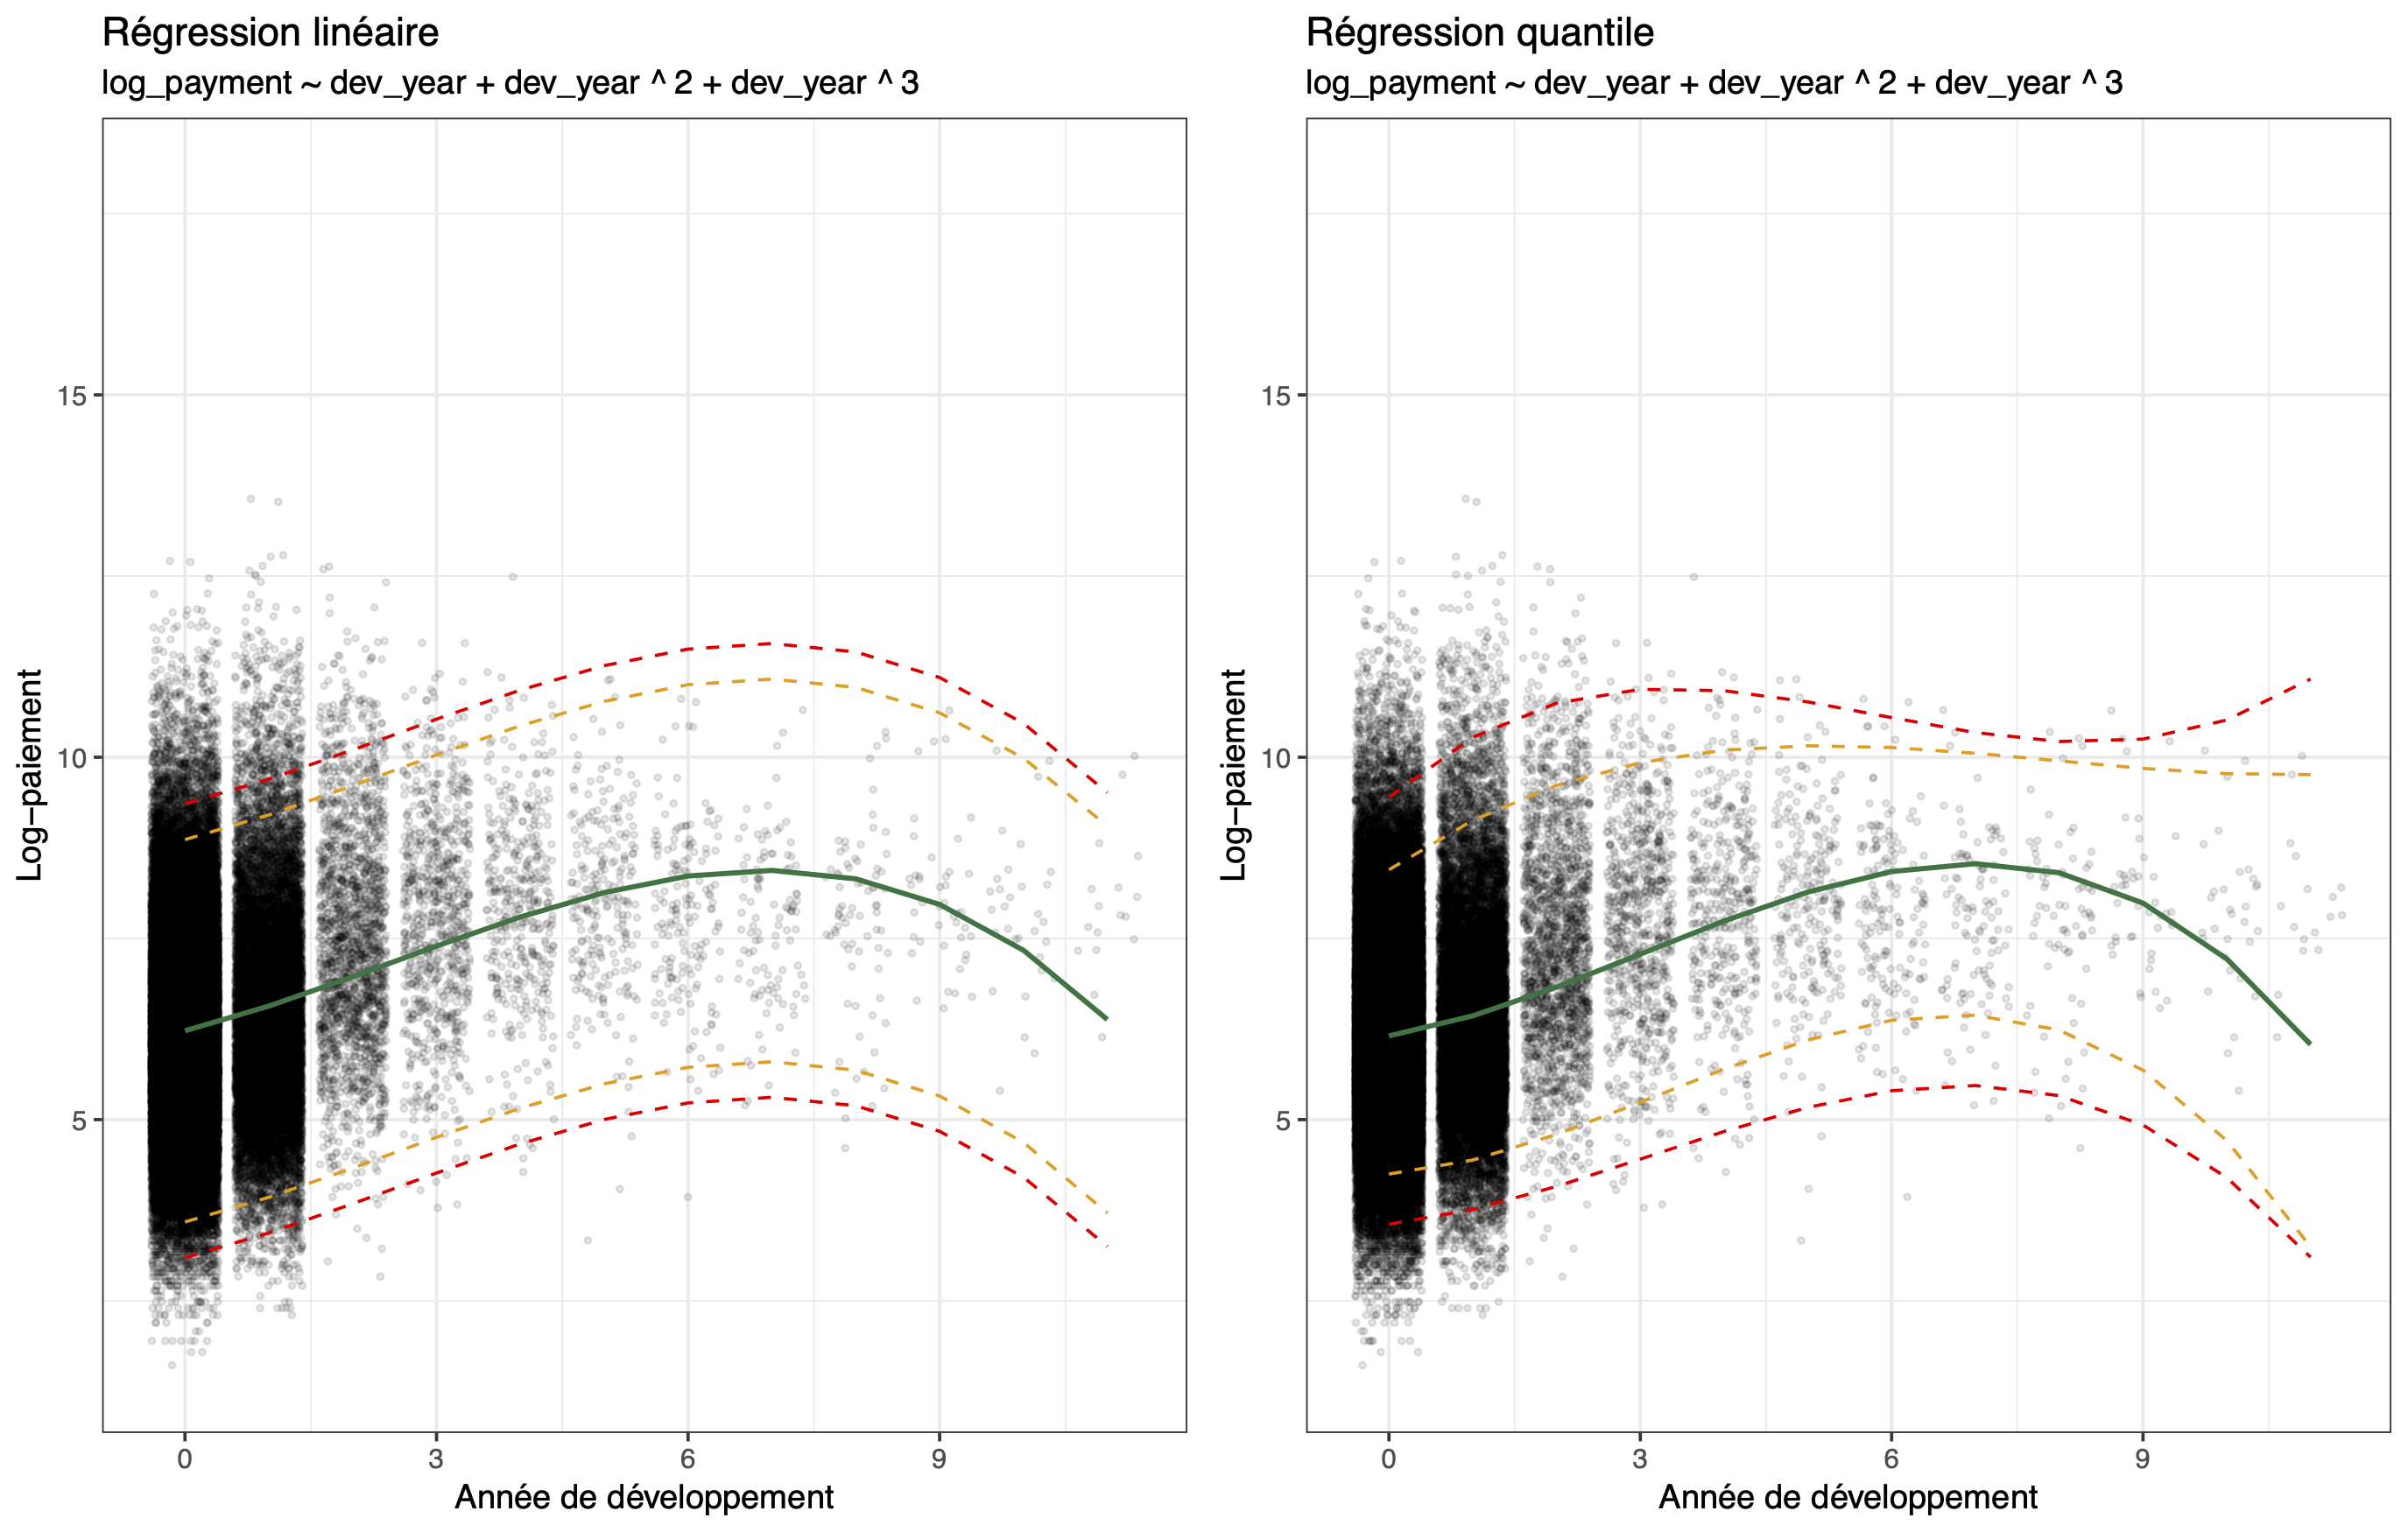
\includegraphics[width = \textwidth]{fit_degre_3.png}
%     \end{figure}
    
% \end{frame}

% ----------

\begin{frame}{Validation des modèles catégoriels}

    \begin{figure}
        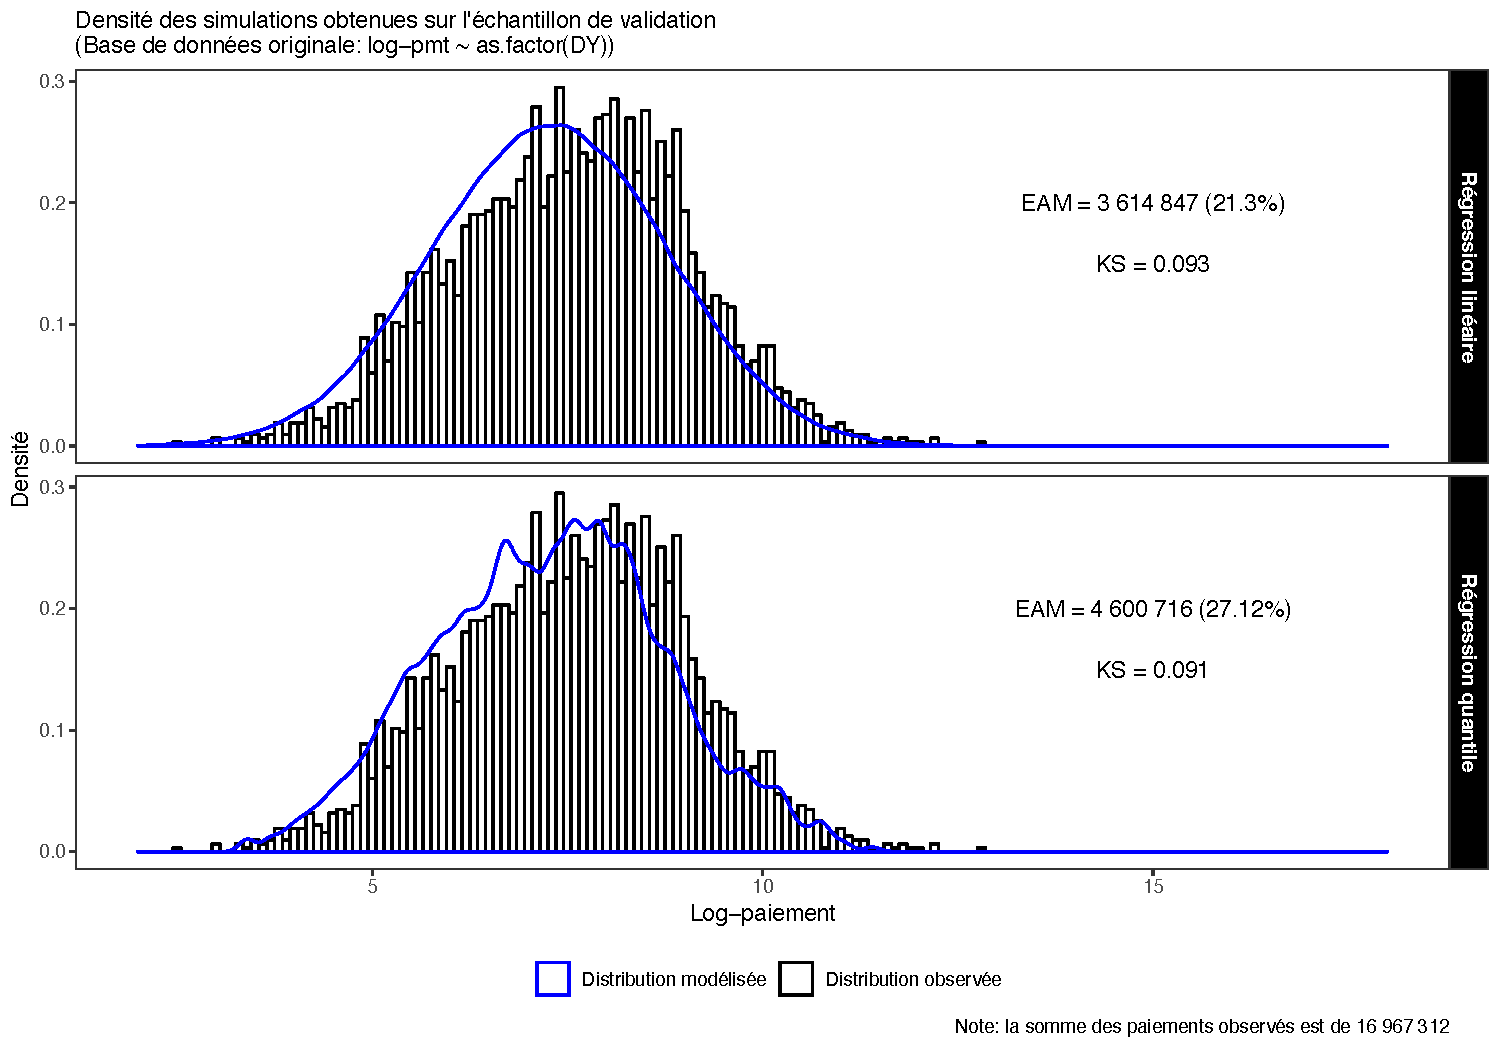
\includegraphics[width = 0.95\textwidth]{plots_valid_lm_rq_fac.pdf}
    \end{figure}

\end{frame}

% ----------

\begin{frame}{Validation des modèles linéaires}

    \begin{figure}
        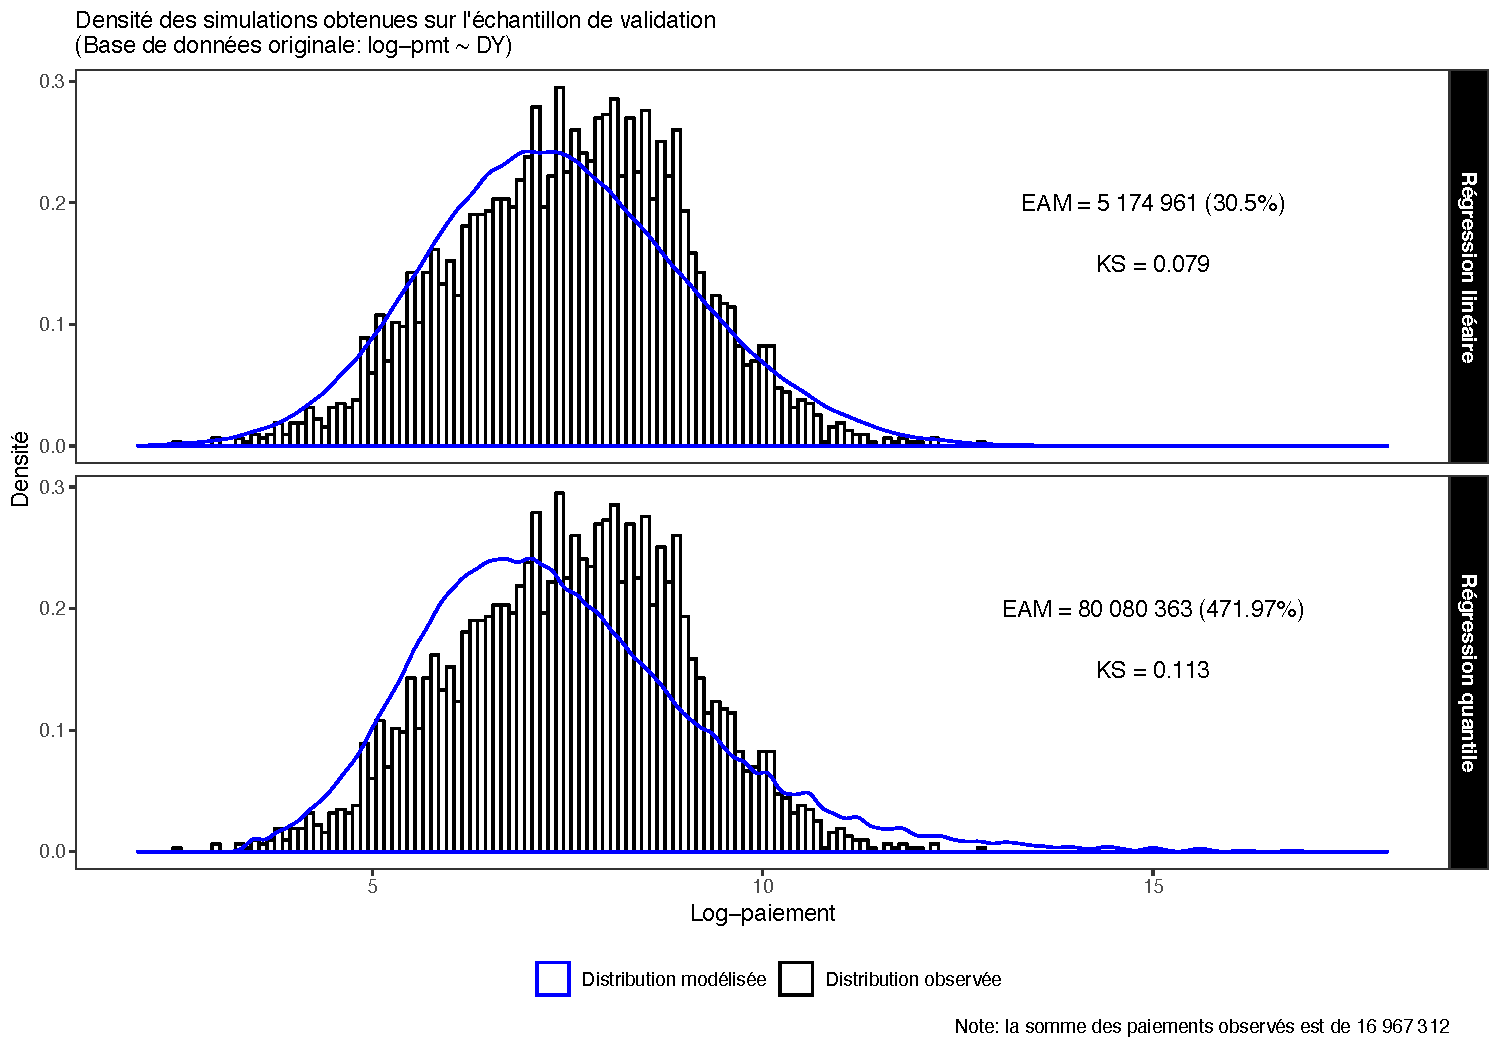
\includegraphics[width = 0.95\textwidth]{plots_valid_lm_rq_degre_1.pdf}
    \end{figure}

\end{frame}

% ----------

\begin{frame}{Validation des modèles quadratiques}

\begin{figure}
    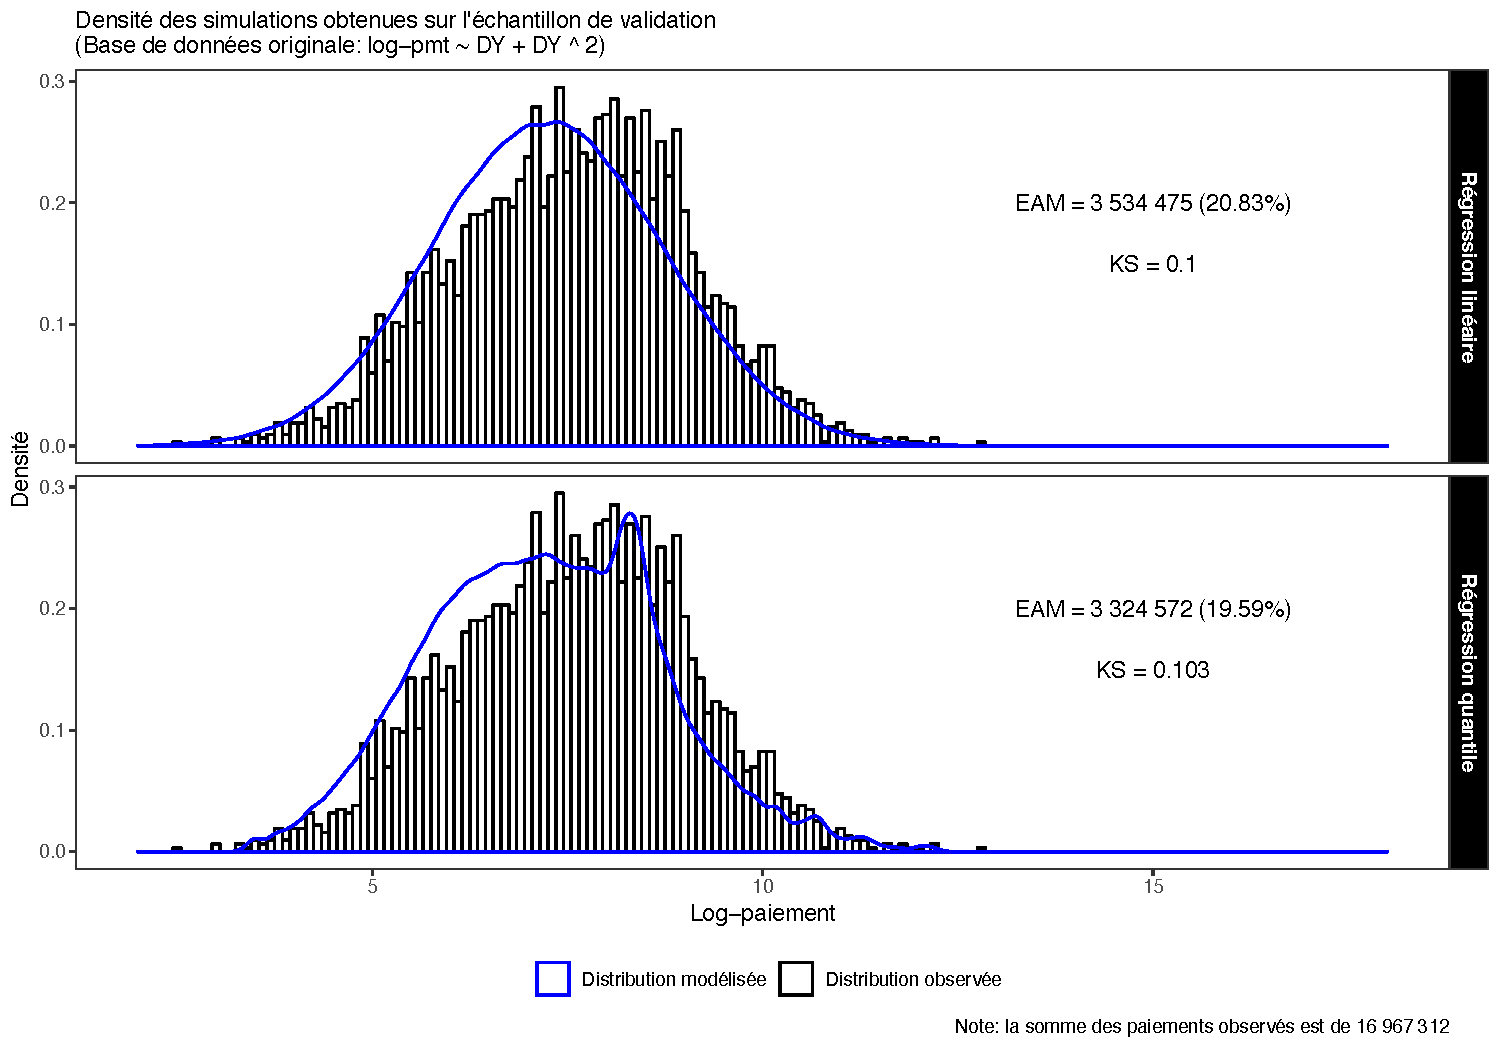
\includegraphics[width = 0.95\textwidth]{plots_valid_lm_rq_degre_2.pdf}
\end{figure}

\end{frame}

% ----------

% \begin{frame}{Validation des modèles cubiques}

% \begin{figure}
%     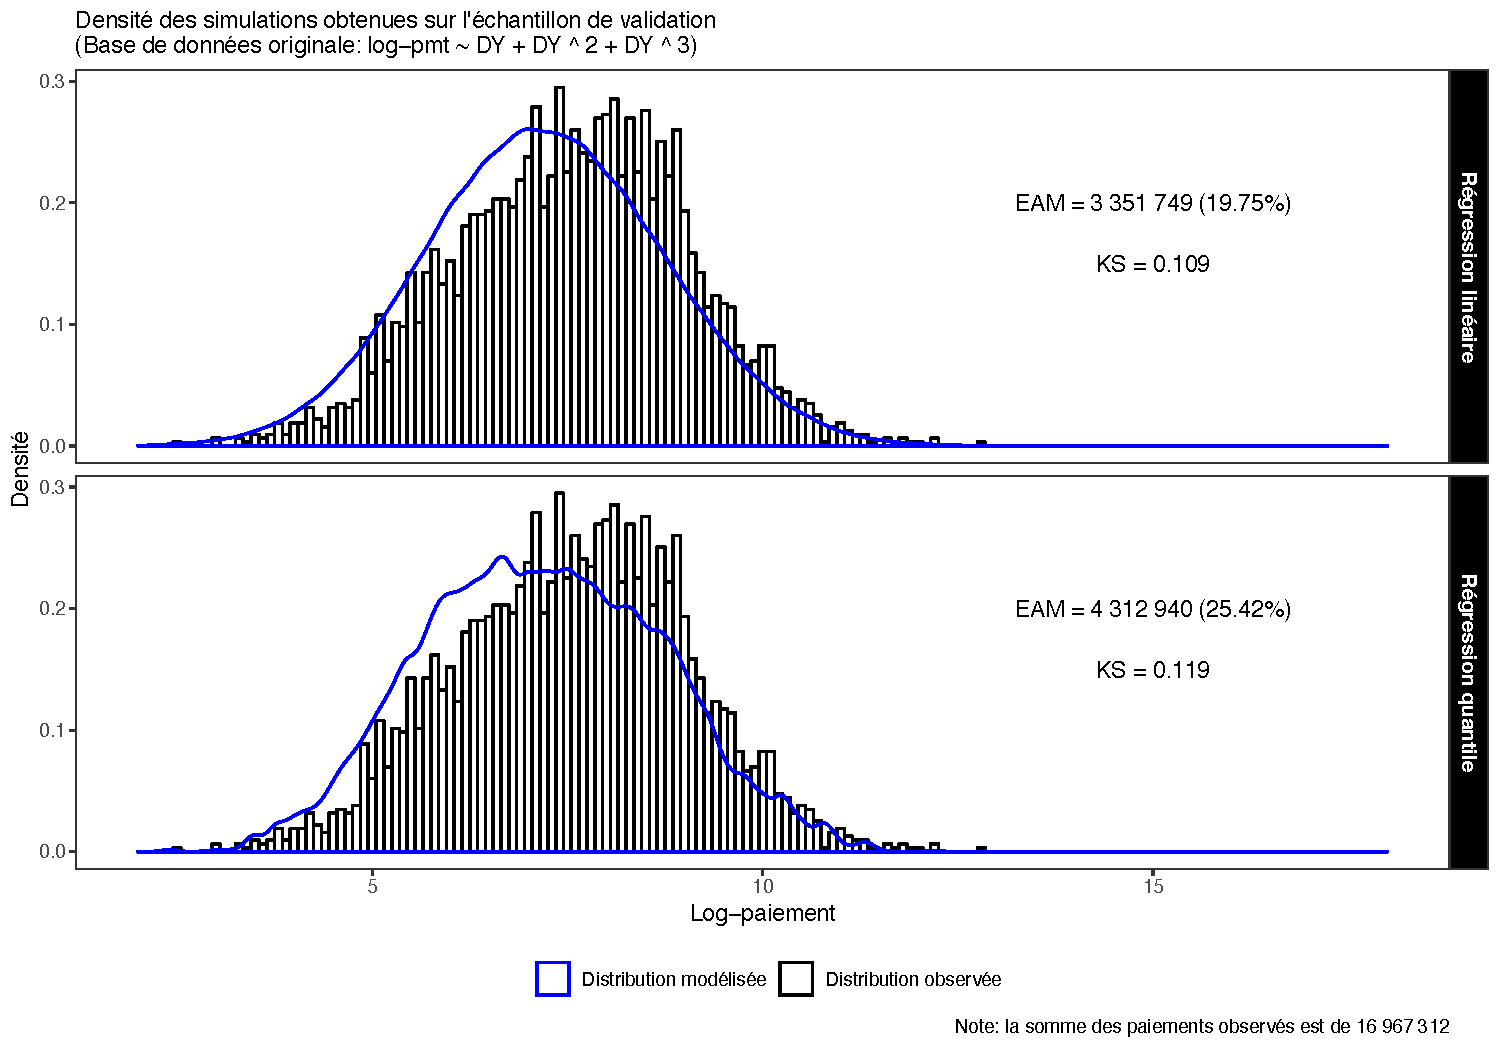
\includegraphics[width = 0.95\textwidth]{plots_valid_lm_rq_degre_3.pdf}
% \end{figure}

% \end{frame}

% ----------

\begin{frame}{Données d'entrainement et de validation}

\begin{itemize}
    \fleche Multiplication par 1000 de 5\% des paiements pris au hasard.
\end{itemize}

\begin{figure}
    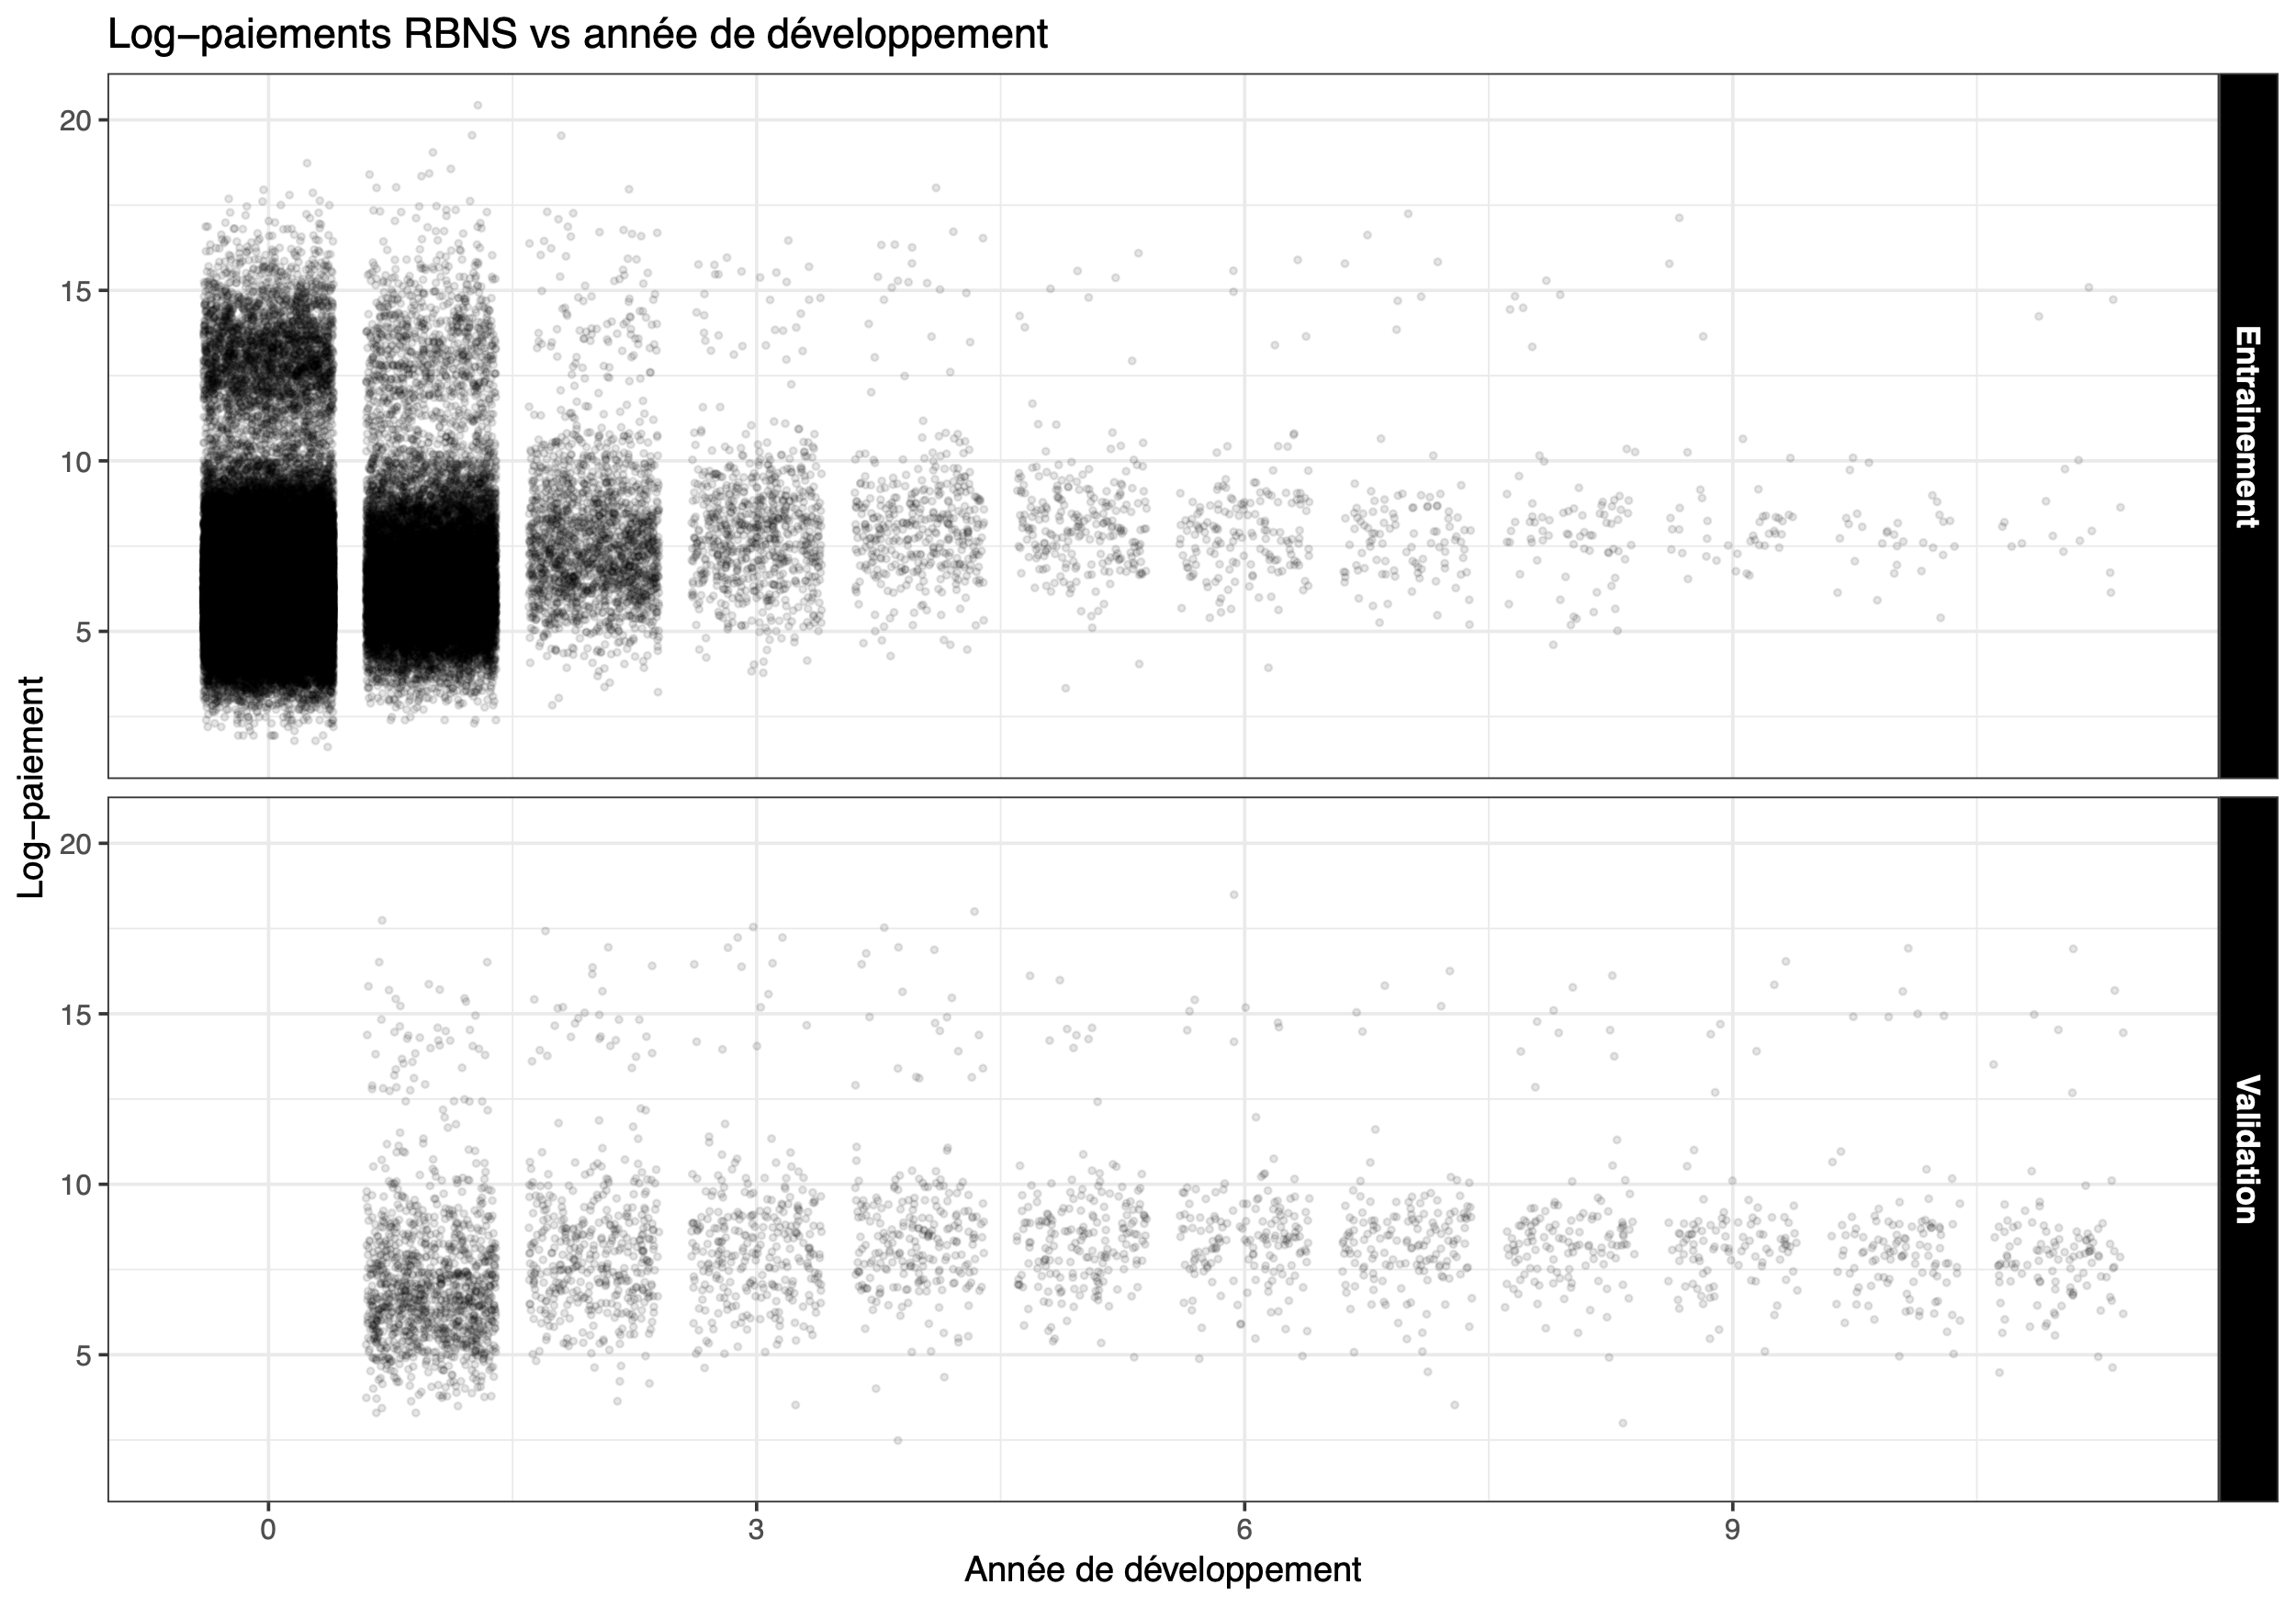
\includegraphics[width = 0.86\textwidth]{nuage_points_ab_overleaf.png}
\end{figure}

\end{frame}

% ----------

\begin{frame}{Entrainement des modèles linéaires}

\begin{figure}
    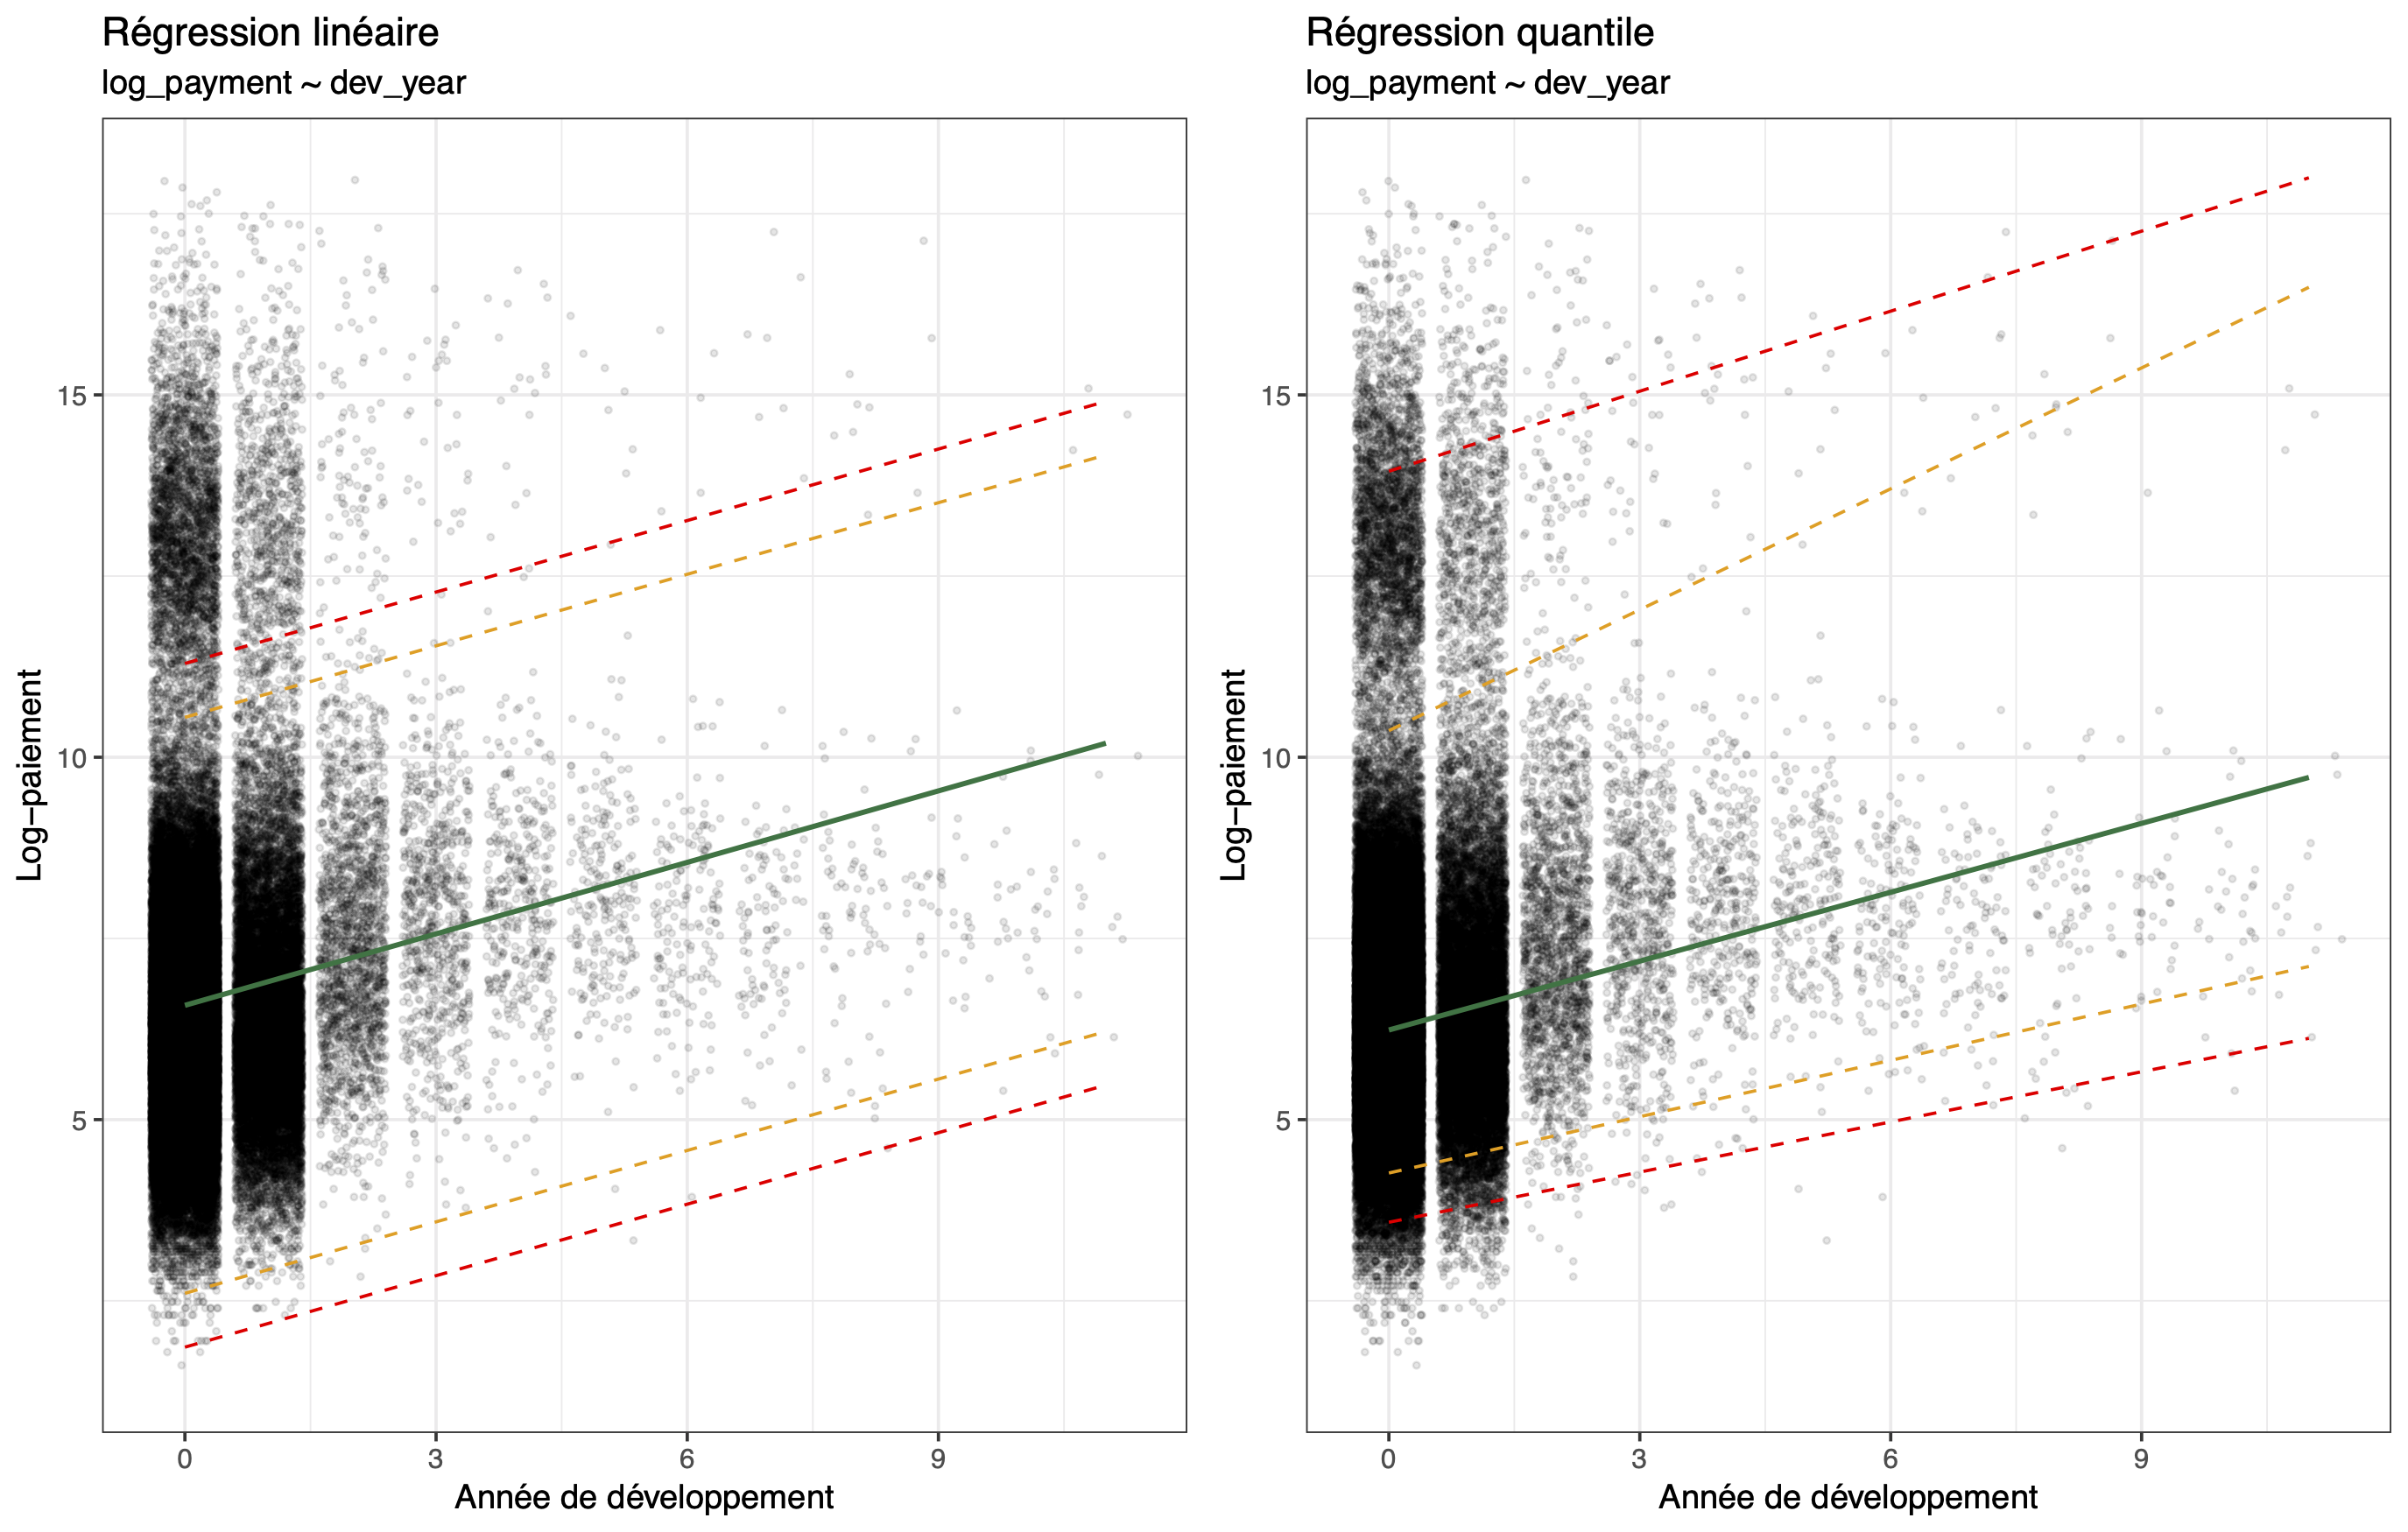
\includegraphics[width = 0.95\textwidth]{fit_degre_1_ab.png}
\end{figure}

\end{frame}

% ----------

\begin{frame}{Validation des modèles linéaires}

\begin{figure}
    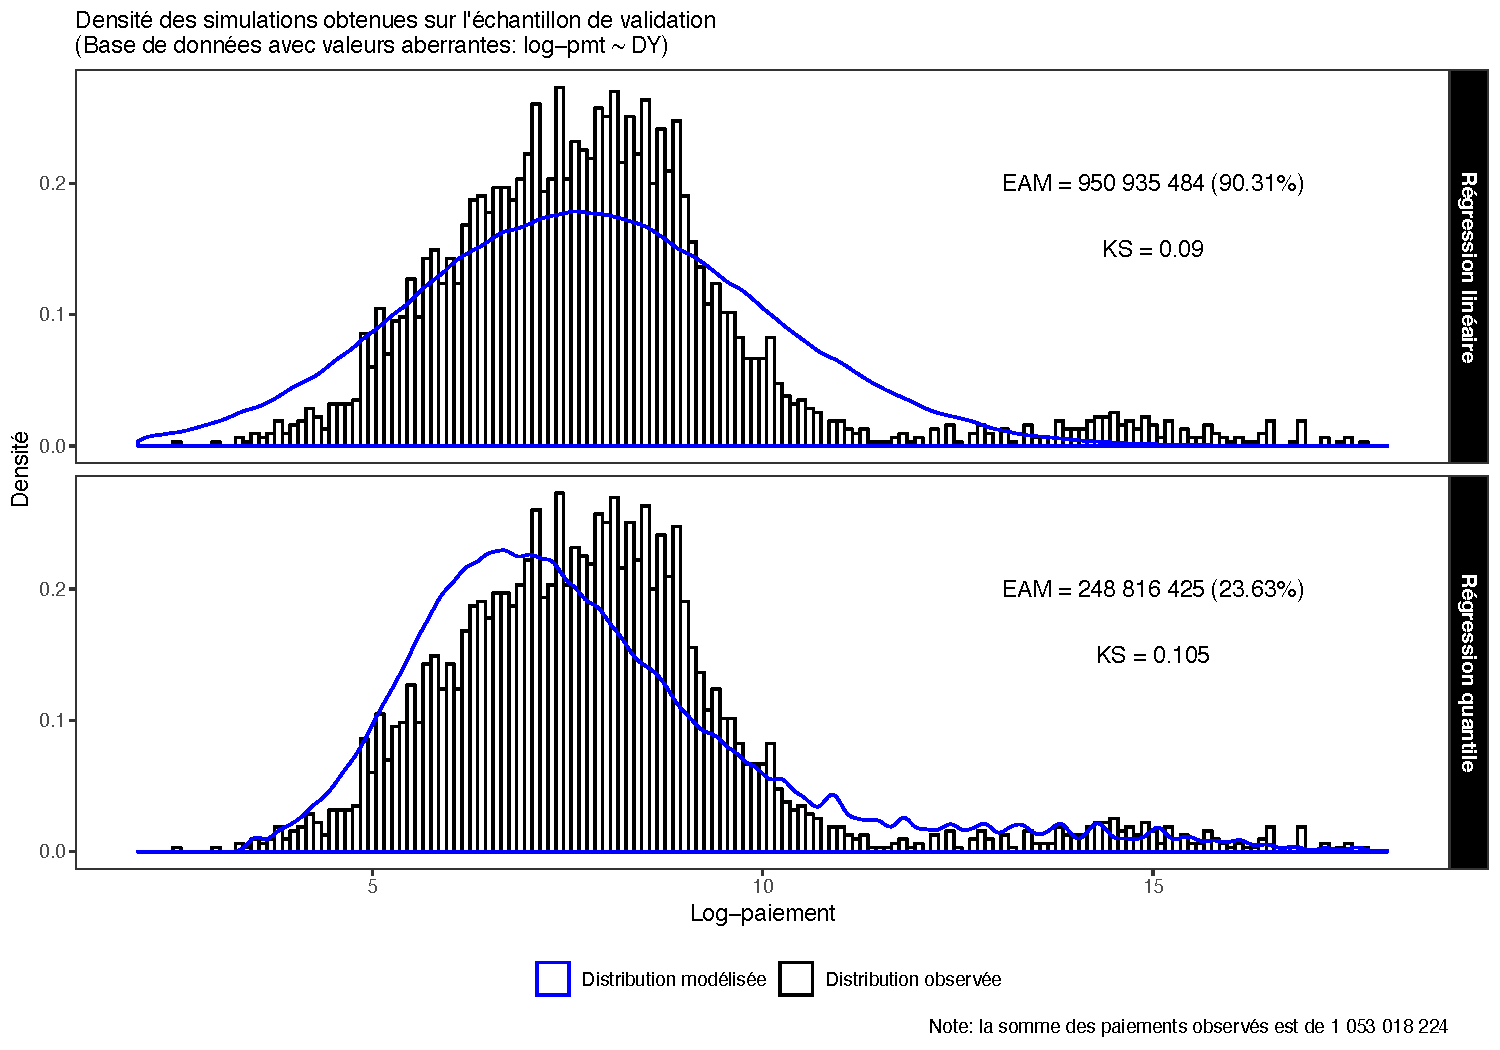
\includegraphics[width = \textwidth]{plots_valid_lm_rq_degre_1_ab.pdf}
\end{figure}

\end{frame}

% ----------

\begin{frame}{Résultats -- Données originales}

\begin{figure}
    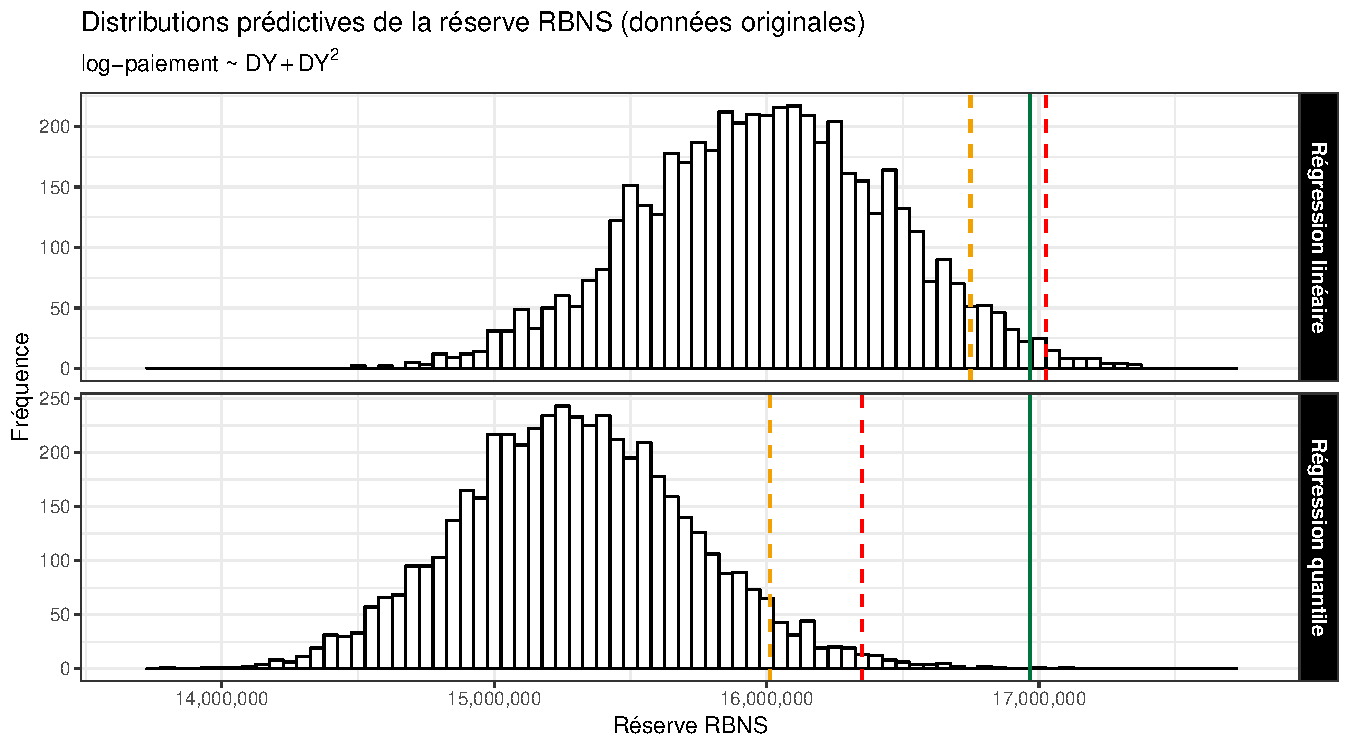
\includegraphics[width = 1.03\textwidth]{pred_dist_degre_2.pdf}
\end{figure}

\end{frame}

% ----------

\begin{frame}{Résultats -- Données originales (suite)}

\begin{figure}
    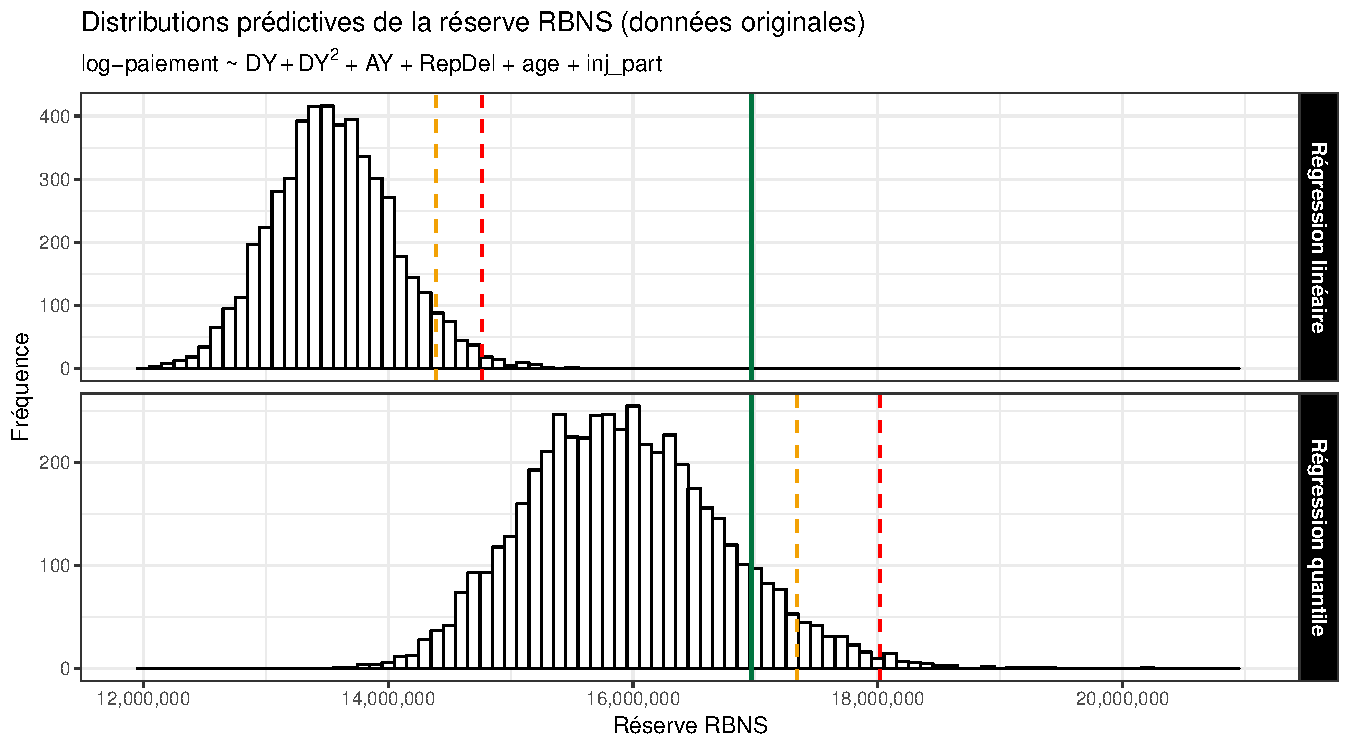
\includegraphics[width = 1.03\textwidth]{pred_dist_all_predictors.pdf}
\end{figure}

\end{frame}

% ----------

\begin{frame}{Résultats -- Données avec valeurs aberrantes}

\begin{figure}
    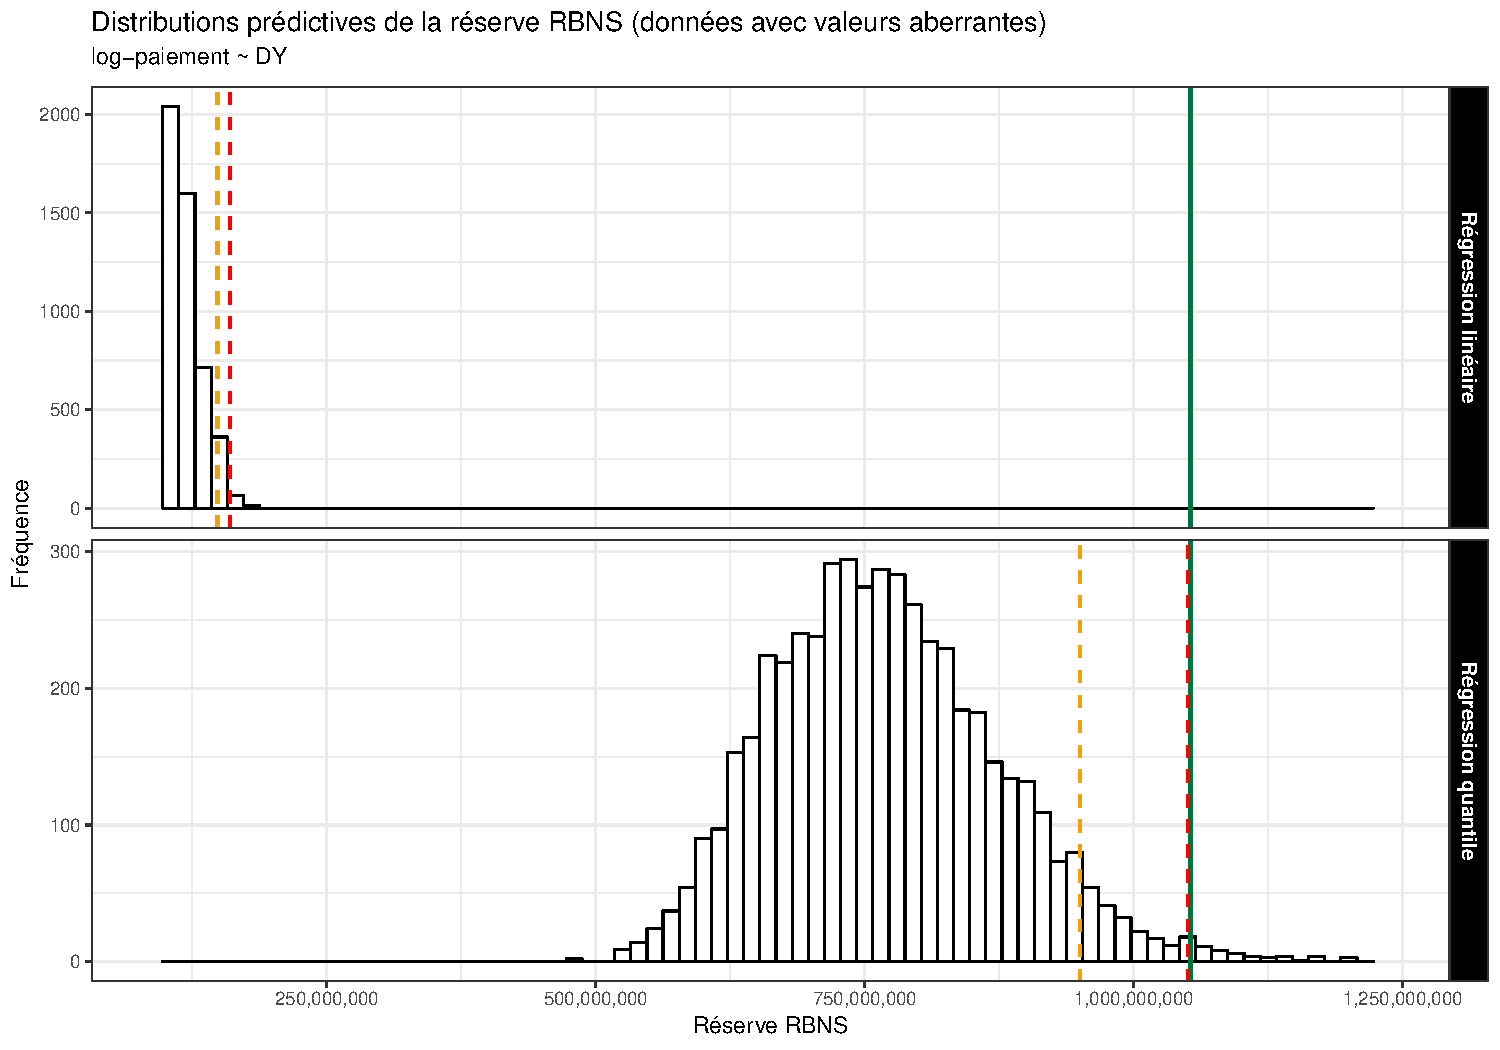
\includegraphics[width = 1.03\textwidth]{pred_dist_degre_1_ab.pdf}
\end{figure}

\end{frame}

% ----------

\begin{frame}{Conclusion}

\begin{itemize}
    \fleche Régression quantile pas significativement meilleure que la régression linéaire sur les données originales.
    \fleche Régression quantile surpasse la régression linéaire selon notre critère sur données avec valeurs aberrantes.
    \fleche L'ajustement de la régression quantile avec modèle linéaire montre qu'on ne peut pas utiliser la régression quantile aveuglément.
    \fleche La statistique de Kolmogorov-Smirnov n'est pas adéquate pour comparer la performance des modèles dans le contexte des réserves.
    \fleche Régression quantile donne des résultats corrects lorsqu'elle est intégrée au modèle d'Antonio et Plat avec tous les prédicteurs.
    \fleche Ne pas oublier que les paiements simulés sont distribués selon une log-normale presque parfaitement, ce qui n'est pas réaliste.
\end{itemize}

\end{frame}

% ----------

\section{Modifications -- Manuel}
\frame{\sectionpage}
% ----------

\begin{frame}{Mise en contexte}
    \begin{itemize}
            \fleche \textbf{Modèle individuel est très malléable}
            \begin{itemize}
                \cercle Processus de Cox (Avanzi et al, 2016).
                \cercle Ajout de copule (Lopez, 2019).
                \cercle Raccorder une distribution Gamma et une distribution Pareto (Reynkens et al., 2016).
            \end{itemize}
            \pause
            \fleche \textbf{Apprentissage supervisé}
            \begin{itemize}
                \cercle Réseaux de neurones (Kuo, 2018).
                \cercle Gradient boosting (Duval et Pigeon, 2019).
            \end{itemize}
    \end{itemize}
\end{frame}

% ----------

\begin{frame}{Mise en contexte}
    \begin{itemize}
            \fleche \textbf{Arbre de décision (Breiman et al.,1984)}
            \begin{itemize}
                \cercle Modèle individuel non paramétrique entièrement basé sur l’utilisation des arbres de décisions (Wüthrich, 2018).
                \cercle Prendre en considération la censure de la variable prédite (Lopez et al., 2016, 2019).
            \end{itemize}
    \end{itemize}
\end{frame}

\begin{frame}{Mise en contexte}

    \begin{exampleblock}{Question guide}
        Est-ce que l’utilisation d’arbres de décision dans la modélisation des paiements peut être une alternative envisageable à l’approche paramétrique?
    \end{exampleblock}

    \begin{alertblock}{Résumé du projet}
        \begin{itemize}
            \fleche Modélisation de la sévérité des paiements avec les arbres de décisions et des ajustements univarié.
        \end{itemize}
    \end{alertblock}
\end{frame}

\begin{frame}{Conception du modèle}
    \begin{itemize}
        \fleche Arbre de décision pour les paiements.
        \fleche Utiliser la classification faite par la division binaire récursive.
        \fleche Pige aléatoire dans les paiements de la base de données qui respectent chacune des conditions menant à cette feuille.
    \end{itemize}
\end{frame}

\begin{frame}{Conception du modèle}
    \begin{itemize}
        \fleche Règle binaire (continue):
             \begin{align*}
                R_1(b,c) &= \{ X_1 \cdots X_B | X_b \leq c \} \\
                R_2(b,c) &= \{ X_1 \cdots X_B | X_b > c \} \text{ .}
            \end{align*}
    \pause
        \fleche Règle binaire (factorielle):
            \begin{align*}
            R_1(b,c) &= \{ X_1 \cdots X_B | X_b \in c \} \\
            R_2(b,c) &= \{ X_1 \cdots X_B | X_b \notin c \} \text{ .}
            \end{align*}
    \end{itemize}
\end{frame}

\begin{frame}{Conception du modèle}
    \begin{itemize}
        \fleche La fonction objective utilisée est la somme des erreurs au carré (SEC):
             \begin{align*}
    \overline{P} &= \frac{1}{q_{\text{total}}} \sum_{q \geq 1} P_{q} \\
    \text{SEC} &= \sum_{q \geq 1}\left(\overline{P} - P_{q}\right)^{2} \text{,} 
\end{align*}
    \pause
        \fleche Le choix de la covariable $b$ et du $c$ sont ceux qui minimise le SEC suivant:
            \begin{align*}
    \text{SEC} &= \sum_{q \in R_{1}(b,c)}\left(\overline{P}_{R_{1}(b,c)} - P_{q}\right)^{2} + \sum_{q \in R_{2}(b,c)}\left(\overline{P}_{R_{2}(b,c)} - P_{q}\right)^{2} \text{.} 
\end{align*}
    \end{itemize}
\end{frame}

\begin{frame}{Conception du modèle}
    \begin{itemize}
        \fleche \textbf{Problème}
        \begin{itemize}
            \cercle Avoir un arbre de décision trop développé ne nous aide pas.
            \cercle Il faut garder un aspect d'aléatoire lors de la simulation des paiements.
        \end{itemize}
        \pause
        \fleche \textbf{Solution}
        \begin{itemize}
            \cercle Ajout de deux conditions à l'arbre de décision pour limiter sa taille:
            \begin{itemize}
                \cercle  Nombre minimal d'observations par feuille.
                \cercle Élagage de l'arbre à l'aide d'un paramètre de complexité à la fonction objective.
             \end{itemize}
        \end{itemize}
    \end{itemize}
\end{frame}

\begin{frame}{Conception du modèle}
    \begin{itemize}
        \fleche  Change une étape au modèle d'Antonio et Plat (2014):
        \begin{itemize}
            \cercle Si paiement, une pige aléatoire dans les paiements de la base de données qui respectent chacune des conditions menant à la feuille dans laquelle la réclamation est classifiée.
        \end{itemize}
    \end{itemize}
\end{frame}

\begin{frame}{Conception du modèle}
    \begin{itemize}
        \fleche \mathbf{Variante:}
        \begin{itemize}
            \cercle Ajustement univarié des paiements à l'intérieur de chaque feuille.
            \cercle Log normal, Gamma et Pareto.
            \cercle Méthode du maximum de vraisemblance.
            \cercle Le choix de la distribution pour chaque feuille est déterminé à l'aide du critère du BIC.
        \end{itemize}
        \pause
        \fleche Si paiement, alors il y a une réalisation de la loi de probabilité associée à la feuille dans laquelle la réclamation est classifiée.
    \end{itemize}
\end{frame}

\begin{frame}{Adaptation du modèle aux données simulées}
    \begin{itemize}
        \fleche \mathbf{Identique à l'exception de:}
        \begin{itemize}
            \cercle 250 000 observations.
            \cercle La date d'évaluation est le 31 décembre 2000. (140 871 observations)
            \cercle Séparé en deux groupes:
            \begin{itemize}
                \cercle secteurs d'affaires 1 et 4,
                \cercle secteurs d'affaires 2 et 3.
            \end{itemize}
        \end{itemize}
        \pause
    \fleche Le choix des variables:
    \begin{itemize}
        \cercle \textit{age};
        \cercle \textit{cc};
        \cercle \textit{inj\textunderscore part}; et 
        \cercle \textit{time}
    \end{itemize}
\end{itemize}
\end{frame}

\begin{frame}{Adaptation du modèle aux données simulées}
\begin{table}[!h]
    \centering
    \begin{tabular}{l c c c c c}
    \hline
     & Moyenne & Médiane & Min & Max & \\
    \hline
    SdA 1 et 4 & 904.88 & 326 & 3.59 & 245 820 & \\
    SdA 2 et 3 & 4575.724 & 1438.80 & 16.17 & 908 429.22 &  \\
    \hline
    \\
    \hline
     & 5\% & 25\% & 75\% & 95\% & 99\% \\
     \hline
     SdA 1 et 4 & 55 & 156.36 & 721.48 & 2928.98 & 10 056.60 \\
     SdA 2 et 3 & 222.64 & 664.62 & 3289.24 & 14 436.61 & 58 985.51 \\
     \hline
    \end{tabular}
    \caption{Caractéristiques des paiements observés dans chaque groupe de secteurs d'activités.}
    \label{tab_pay_den}
\end{table}
\end{frame}

\frame{
\frametitle{Application numérique}
\begin{itemize}
    \fleche Modélisation des paiements à l'aide d'arbres de décisions.
    \pause
    \fleche En excluant les évènements où il n'y a aucun paiement:
    \begin{itemize}
        \cercle 75 515 paiements pour les secteurs d'affaires $\{1,4\}$.
        \cercle 33 703 paiements pour les secteurs d'affaires $\{2,3\}$.
    \end{itemize}
\end{itemize} 
}

\frame{
\frametitle{Application numérique}
\begin{itemize}
    \fleche Le choix du nombre d'observations minimales:
    \begin{itemize}
        \cercle Le choix du nombre d'observations minimales:
        \begin{itemize}
            \cercle Par validation croisée.
            \cercle À l'aide de la statistique \textit{xerror}. 
        \end{itemize}
        \pause
        \cercle Pour le groupe $\{1,4\}$, les feuilles doivent contenir au minimum 0.5\% des observations (378).
        \cercle Pour le groupe $\{2,3\}$, au minimum 0.4\% des observations (134).
    \end{itemize}
    \pause
    \fleche Élagage de l'arbre de décision:
    \begin{itemize}
        \cercle Le choix fut de prendre le $\alpha$ qui minimise le \textit{xerror}.
        \pause
        \cercle Le groupe $\{1,4\}$ comporte 33 feuilles.
        \cercle Le groupe $\{2,3\}$ comporte 32 feuilles.
    \end{itemize}
\end{itemize} 

}

\frame{
\frametitle{Application numérique}
\begin{itemize}
    \fleche Ajustement univarié:
    \begin{itemize}
        \cercle Le groupe $\{1,4\}$ comporte uniquement des distributions log normales.
        \cercle Le groupe $\{2,3\}$ a 30 feuilles avec des distributions log normal et 2 feuilles avec des distributions de Pareto.
    \end{itemize}
    \pause
    \fleche Modèle de contrôle:
    \begin{itemize}
        \cercle Modèle linéaire généralisé (MLG).
        \cercle Mêmes variables que dans les arbres de décisions.
    \end{itemize}
\end{itemize} 

}

\frame{
\frametitle{Application numérique}
\begin{itemize}
    \fleche Librairies en R:
    \begin{itemize}
        \cercle actuar
        \cercle fitdistrplus
        \cercle parallel
        \cercle pbapply
        \cercle rpart
        \cercle rpart.plot
        \cercle treeClust
    \end{itemize}
\end{itemize} 
}
\frame{
\frametitle{Application numérique}
\begin{itemize}
    \fleche Étapes pour la simulation du paiements
    \begin{itemize}
        \item \textbf{1.} Déterminer les hyperparamètres pour l'arbre.
        \item \textbf{2.} Construire l'arbre et l'élaguer.
        \item \textbf{3.} Pour chaque paiement dans notre base de données de paiements, prédire la feuille dans laquelle il sera.
        \item \textbf{4.} Lorsqu'un paiement doit être simulé pour une réclamation à un temps $t$, à l'aide des variables explicatives liées à la réclamation et le temps $t$ du paiement, prédire la feuille dans laquelle le nouveau paiement sera. 
        \item \textbf{5.} Faire une pige dans le vecteur de paiements correspondant.
    \end{itemize}
\end{itemize} 
}

\frame{
\frametitle{Application numérique}
\begin{itemize}
    \fleche Étapes pour la simulation du paiements - Variante
    \begin{itemize}
        \item \textbf{1.} Déterminer les hyperparamètres pour l'arbre.
        \item \textbf{2.} Construire l'arbre et l'élaguer.
        \item \textbf{3.} Pour chaque paiement dans notre base de données de paiements, prédire la feuille dans laquelle il sera.
        \item \textcolor{blue}{\textbf{4.} Pour chaque feuille, faire un ajustement univarié à l'aide de divers lois. Enregistrer les paramètres et la loi dans une base de données. }
        \item \textbf{5.} Lorsqu'un paiement doit être simulé pour une réclamation à un temps $t$, à l'aide des variables explicatives liées à la réclamation et le temps $t$ du paiement, prédire la feuille dans laquelle le nouveau paiement sera. 
        \item \textcolor{blue}{\textbf{6.} Selon la feuille, simuler une réalisation de la distribution calculée à l'étape 4.}
    \end{itemize}
\end{itemize} 
}

\frame{
\frametitle{Application numérique}
\begin{figure}[!ht]
   \centering
   \subfloat{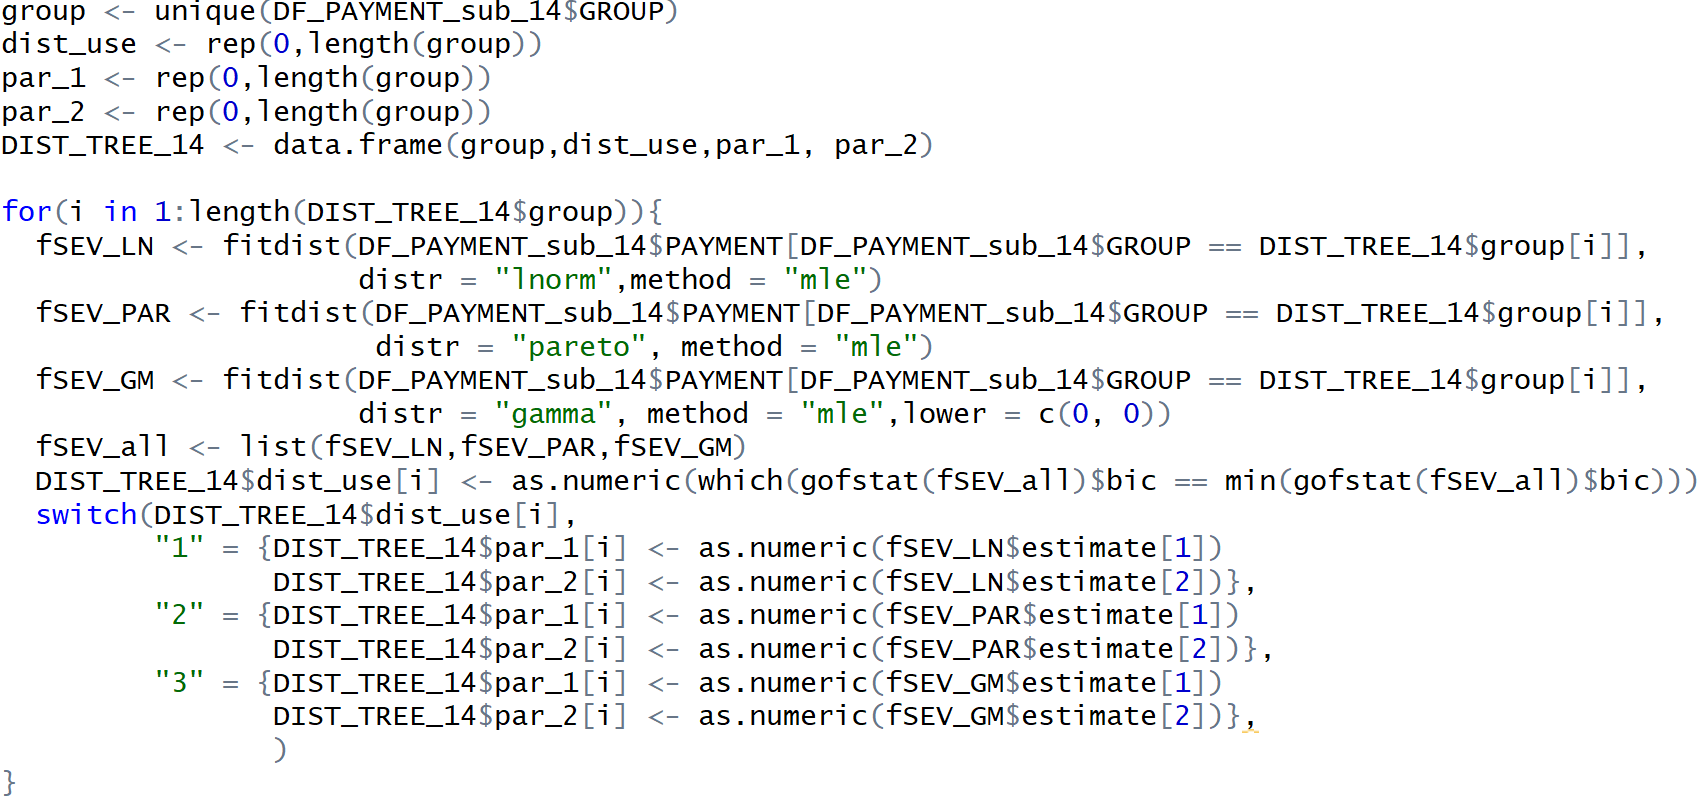
\includegraphics[width=\textwidth]{Stack_Param.PNG}}
   \label{pai_23}
\end{figure}
}

\frame{
\frametitle{Résultats}
\begin{itemize}
    \fleche 10 000 simulations.
    \pause
    \fleche $VaR_{\0.95}$ et $VaR_{\0.99}$.
    \pause
    \fleche $TVaR_{\0.95}$ et $TVaR_{\0.99}$.
\end{itemize}
}

\frame{
\frametitle{Résultats - SdA 1 et 4}
\begin{center}
\setlength{\tabcolsep}{2pt}
     \footnotesize
\begin{tabular}[!h]
    \centering
    \begin{tabular}{c c c c c c c c }
    \hline
      & 1 & 2 & 3 & 4 & 5 & 6 & 7 \\
    \hline
    1994 & 5 267 739 & 2 861 217 & 984 366 & 693 844 & 424 251 & 356 870 & 281 004  \\
    1995 & 5 042 668 & 2 387 215 & 757 507 & 426 723 & 297 264 & 219 686 & \textbf{190 739} \\
    1996 & 5 136 459 & 2 989 370 & 1 114 484 & 656 864 & 421 078 & \textbf{312 076} & \textbf{234 168}  \\
    1997 & 4 698 430 & 2 434 732 & 898 441 & 482 069 & \textbf{340 537} & \textbf{236 044} & \textbf{154 369}  \\
    1998 & 5 032 212 & 2 778 030 & 1 010 774 & \textbf{644 286} & \textbf{444 630} & \textbf{300 657} & \textbf{214 337}  \\
    1999 & 5 031 191 & 2 709 034 & \textbf{1 135 874} & \textbf{623 700} & \textbf{403 146} & \textbf{280 733} & \textbf{183 125}  \\
    2000 & 5 436 820 & \textbf{2 998 817} & \textbf{1 290 701} & \textbf{785 669} & \textbf{530 200} & \textbf{370 414} & \textbf{275 939}  \\
    \hline
    \end{tabular}
    \caption{Triangle incrémental pour les secteurs d'affaires 1 et 4. Les valeurs en gras sont les valeurs des paiements de la base de validation.}
    \label{Tri_14}
\end{tabular}
\end{center}
}

\frame{
\frametitle{Résultats - SdA 1 et 4}
\begin{figure}[!ht]
   \centering
   \subfloat{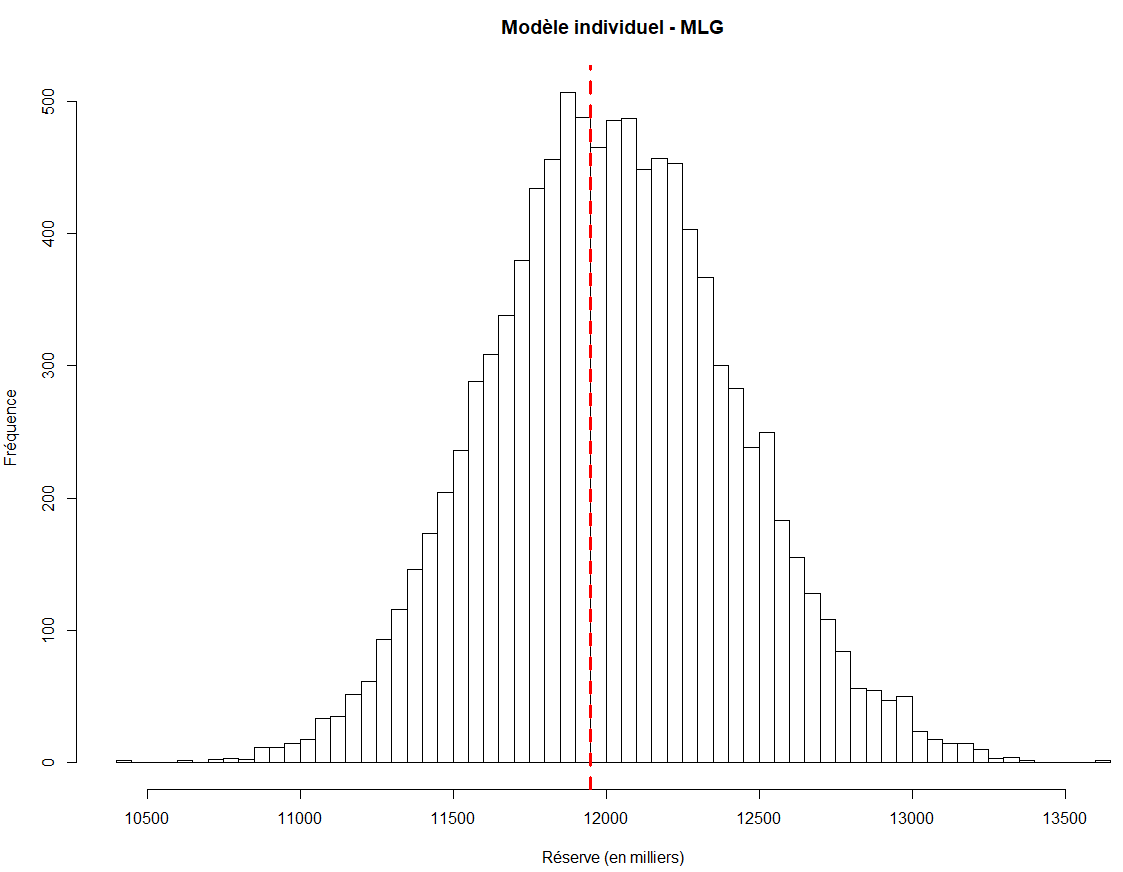
\includegraphics[width=.45\textwidth]{GLM_14.PNG}}\quad
   \subfloat{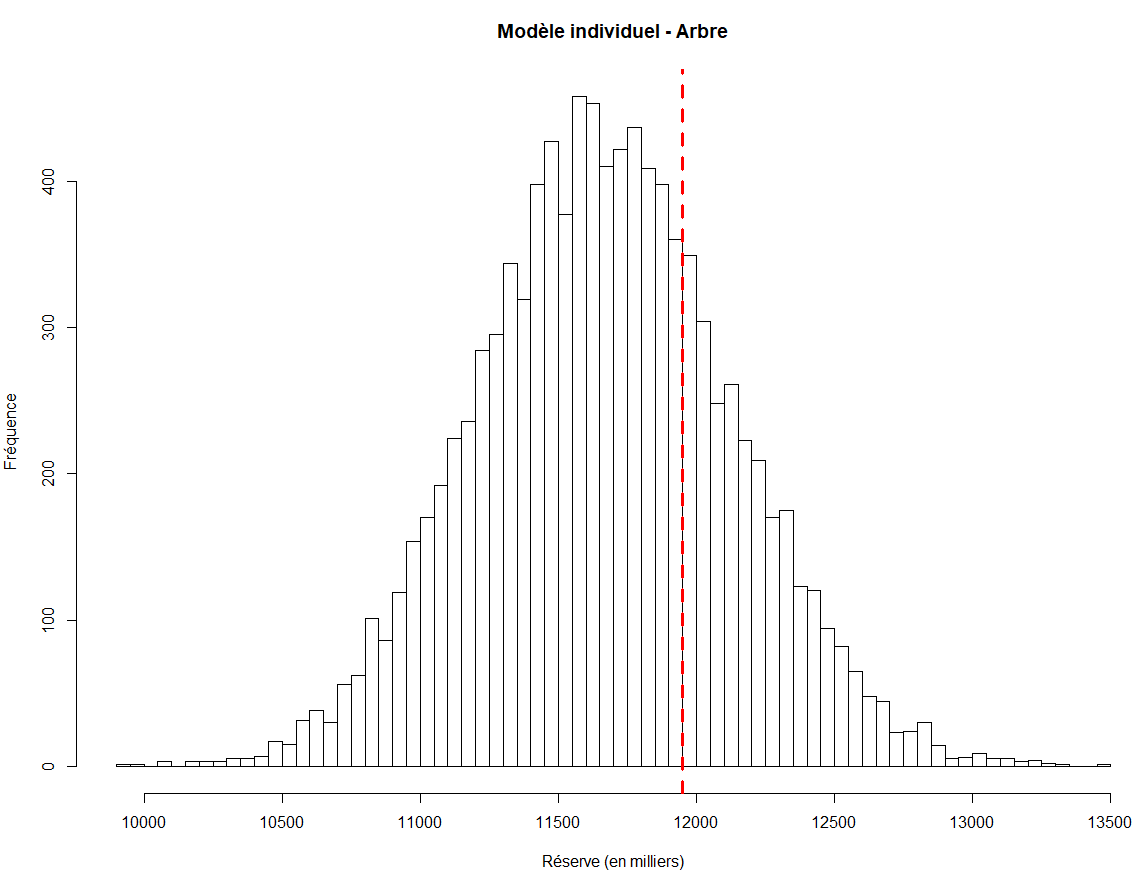
\includegraphics[width=.45\textwidth]{Arbre_14.PNG}}\quad
   \subfloat{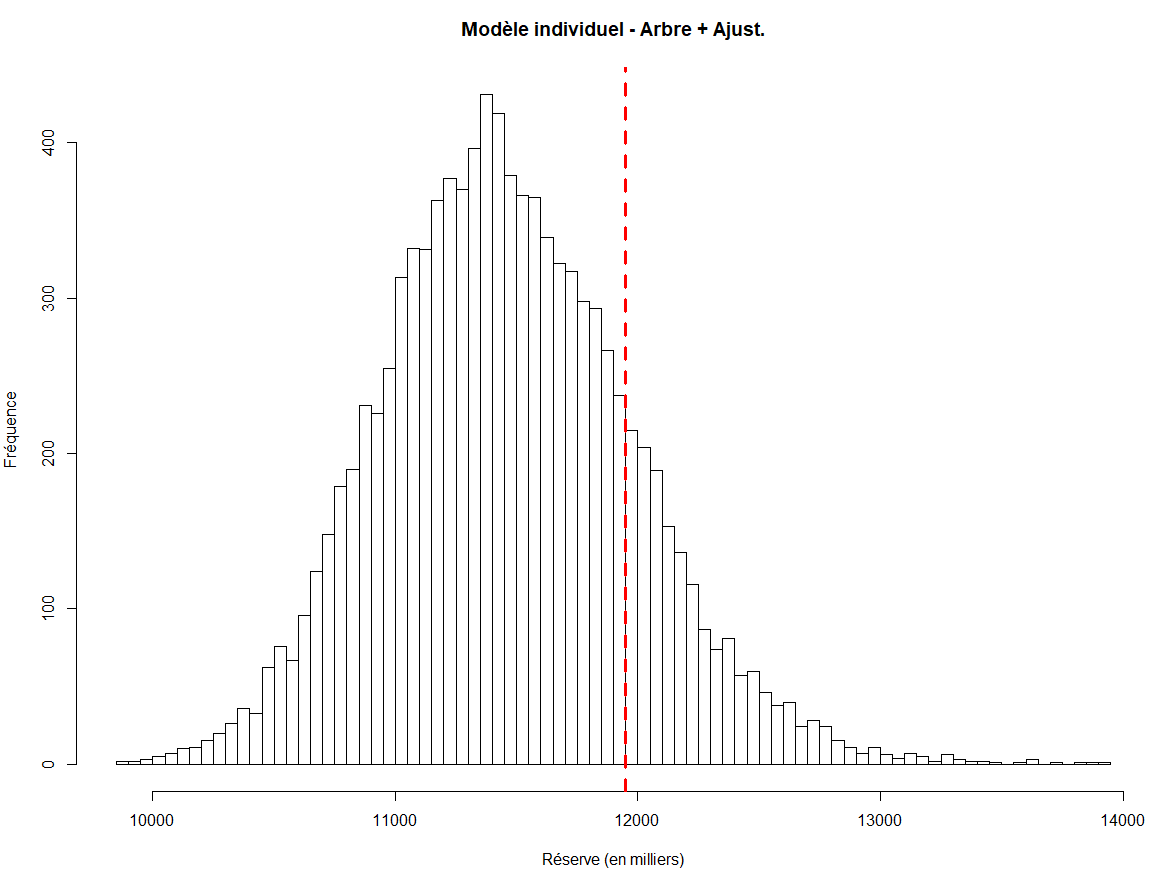
\includegraphics[width=.45\textwidth]{Arbre_Ajust_14.PNG}}\\
   \label{Reserve_14}
\end{figure}
}

\frame{
\frametitle{Résultats - SdA 1 et 4}
\begin{center}
\setlength{\tabcolsep}{2pt}
     \small
\begin{tabular}[!h]
    \centering
    \begin{tabular}{c  c c c c c c}
    \hline
     Modèle & Moyenne & Écart-type & $VaR_{0.95}$ & $VaR_{0.99}$ & $TVaR_{0.95}$ & $TVaR_{0.99}$ \\
    \hline
    Ind. GLM & 12 019.4 & 402.8 & 12 692.5 & 12 987.1 & 12 873.9 & 13 113.1\\
    Ind. Arbre & 11 665.8 & 462.1 & 12 434.7 & 12 760.7 & 12 632.1 & 12 931.0\\
    Ind. Arbre + Ajust. & 11 459.7 & 515.5 & 12 338.8 & 12 776.9 & 12 622.1 & 13 059.9\\
    Observé & 11 950.1 & & & & & \\
    \hline
    \end{tabular}
    \label{Car_Reserve_14}
\end{tabular}
\end{center}
}

\frame{
\frametitle{Résultats - SdA 1 et 4}
\begin{itemize}
    \fleche \textbf{Modèle ind. arbre}
    \begin{itemize}
        \cercle L'échantionnage dans le vecteur empirique impose une borne supérieure aux paiements qui sont simulés.
    \end{itemize}
    \fleche \textbf{Modèle ind. arbre + ajustement}
    \begin{align*}
            &\mathbb{P}\left[P \geq max(p_{R_i}) \right] \leq \frac{1}{\#\{n \in R_i \}}
        \end{align*}
   
\end{itemize}
}

\frame{
\frametitle{Résultats - SdA 2 et 3}
\begin{center}
\setlength{\tabcolsep}{2pt}
     \footnotesize
\begin{tabular}[!h]
    \centering
    \begin{tabular}{c c c c c c c c }
    \hline
      & 1 & 2 & 3 & 4 & 5 & 6 & 7 \\
    \hline
    1994 & 13 817 499 & 6 125 217 & 1 892 641 & 935 175 & 445 483 & 475 312 & 358 699  \\
    1995 & 12 134 574 & 5 836 604 & 2 185 736 & 847 248 & 535 249 & 335 117 & \textbf{233 806} \\
    1996 & 12 013 964 & 7 509 183 & 3 185 326 & 1 522 286 & 853 380 & \textbf{656 966} & \textbf{458 252}  \\
    1997 & 12 189 174 & 7 140 726 & 3 221 795 & 1 412 041 & \textbf{812 177} & \textbf{541 987} & \textbf{405 723}  \\
    1998 & 10 321 082 & 5 392 646 & 1 571 823 & \textbf{678 902} & \textbf{398 893} & \textbf{277 442} & \textbf{230 762}  \\
    1999 & 12 409 959 & 7 809 218 & \textbf{2 752 899} & \textbf{1 222 011} & \textbf{643 754} & \textbf{405 577} & \textbf{366 801}  \\
    2000 & 10 802 693 & \textbf{4 603 907} & \textbf{1 450 900} & \textbf{664 911} & \textbf{365 487} & \textbf{281 374} & \textbf{154 630}  \\
    \hline
    \end{tabular}
    \label{Tri_14}
\end{tabular}
\end{center}
}

\frame{
\frametitle{Résultats - SdA 2 et 3}
\begin{figure}[!ht]
   \centering
   \subfloat{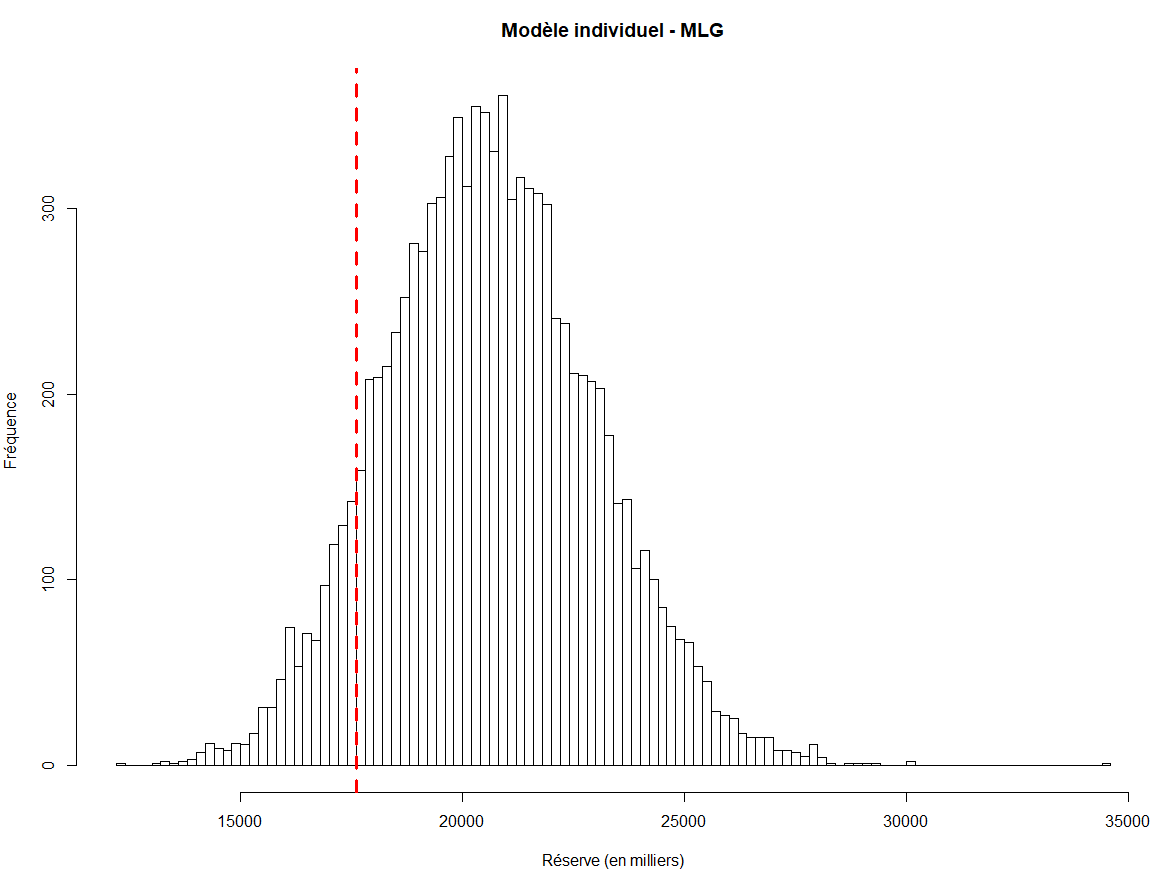
\includegraphics[width=.45\textwidth]{GLM_23.PNG}}\quad
   \subfloat{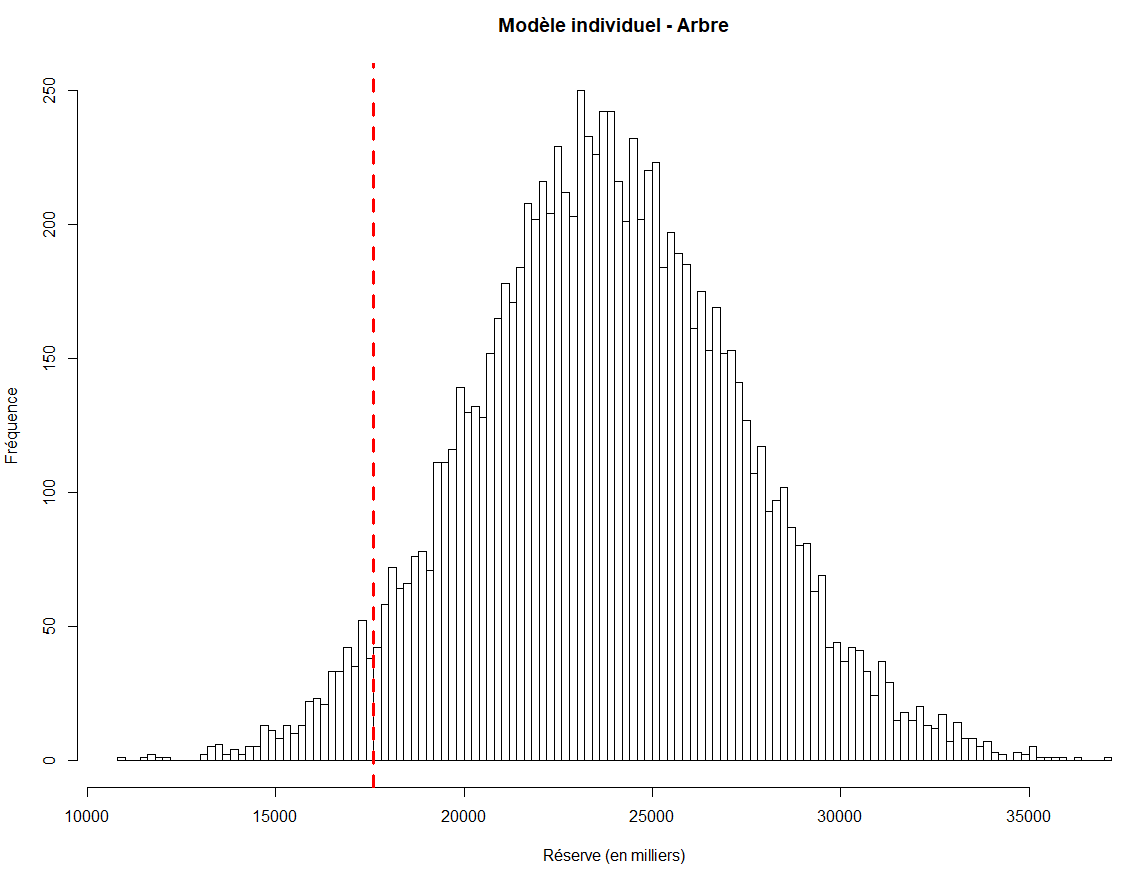
\includegraphics[width=.45\textwidth]{Arbre_23.PNG}}\quad
   \subfloat{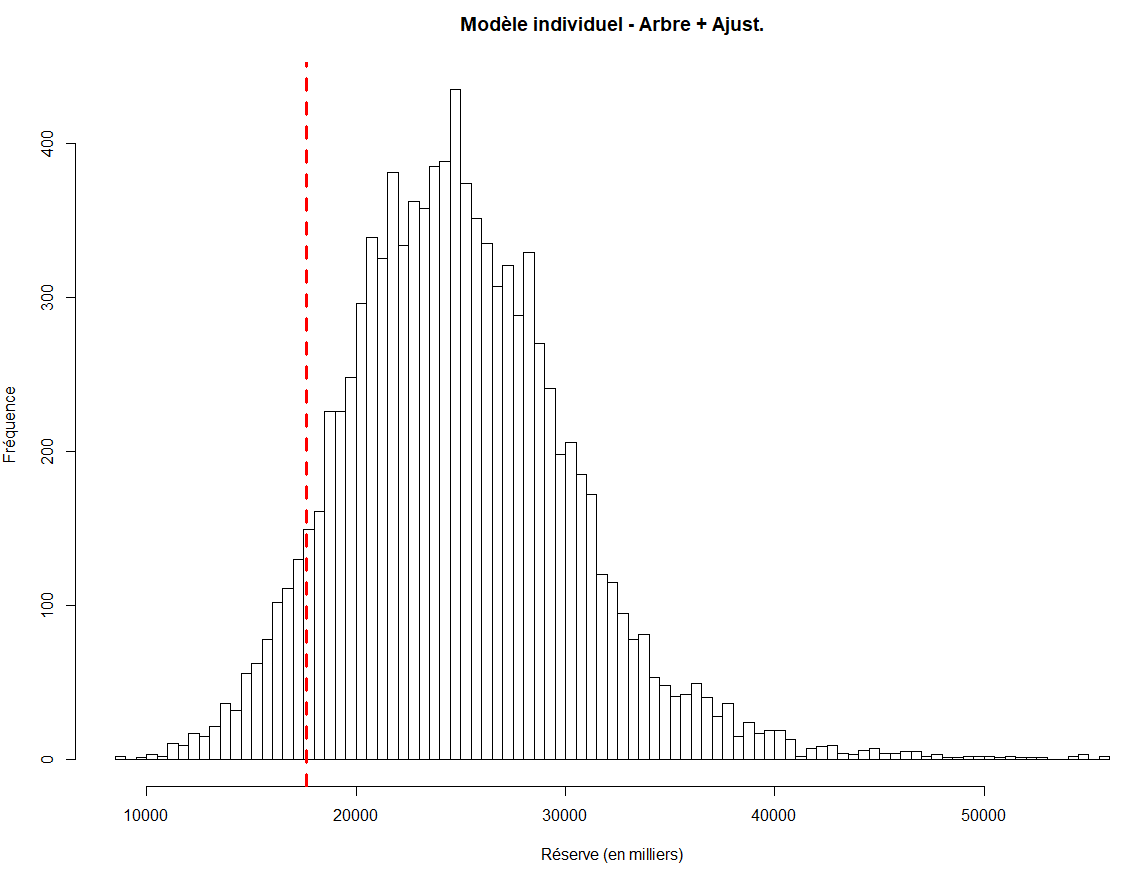
\includegraphics[width=.45\textwidth]{Arbre_Ajust_23.PNG}}\\
   \label{Reserve_23}
\end{figure}
}

\frame{
\frametitle{Résultats - SdA 2 et 3}
\begin{center}
\setlength{\tabcolsep}{2pt}
     \small
\begin{tabular}[!h]
    \centering
    \begin{tabular}{c c c c c c c}
    \hline
     Modèle & Moyenne & Écart-type & $VaR_{0.95}$ & $VaR_{0.99}$ & $TVaR_{0.95}$ & $TVaR_{0.99}$ \\
    \hline
    Ind. GLM & 20 618.8 & 2348.0 & 24 601.9 & 26 317.8 & 25 668.9 & 27 309.6\\
    Ind. Arbre & 23 798.8 & 3546.4 & 29 642.8 & 32 359.7 & 31 287.9 & 33 475.5\\
    Ind. Arbre + Ajust. & 24 969.3 & 5513.7 & 34 359.0 & 40 629.9 & 38 583.0 & 45 500.7\\
    Observé & 17 607.1 & & & & & \\
    \hline
    \end{tabular}
    \label{Car_Reserve_14}
\end{tabular}
\end{center}
}

\begin{frame}{Résultats - SdA 2 et 3}
\begin{table}[!h]
    \centering
    \begin{tabular}{l c c c c c}
    \hline
     & Moyenne & Médiane & Min & Max & \\
    \hline
    SdA 1 et 4 & 904.88 & 326 & 3.59 & 245 820 & \\
    SdA 2 et 3 & 4575.724 & 1438.80 & 16.17 & 908 429.22 &  \\
    \hline
    \\
    \hline
     & 5\% & 25\% & 75\% & 95\% & 99\% \\
     \hline
     SdA 1 et 4 & 55 & 156.36 & 721.48 & 2928.98 & 10 056.60 \\
     SdA 2 et 3 & 222.64 & 664.62 & 3289.24 & 14 436.61 & 58 985.51 \\
     \hline
    \end{tabular}
    \caption{Caractéristiques des paiements observés dans chaque groupe de secteurs d'activités.}
    \label{tab_pay_den}
\end{table}
\end{frame}

\frame{
\frametitle{Résultats - SdA 2 et 3}
\begin{figure}[!ht]
   \centering
   \subfloat{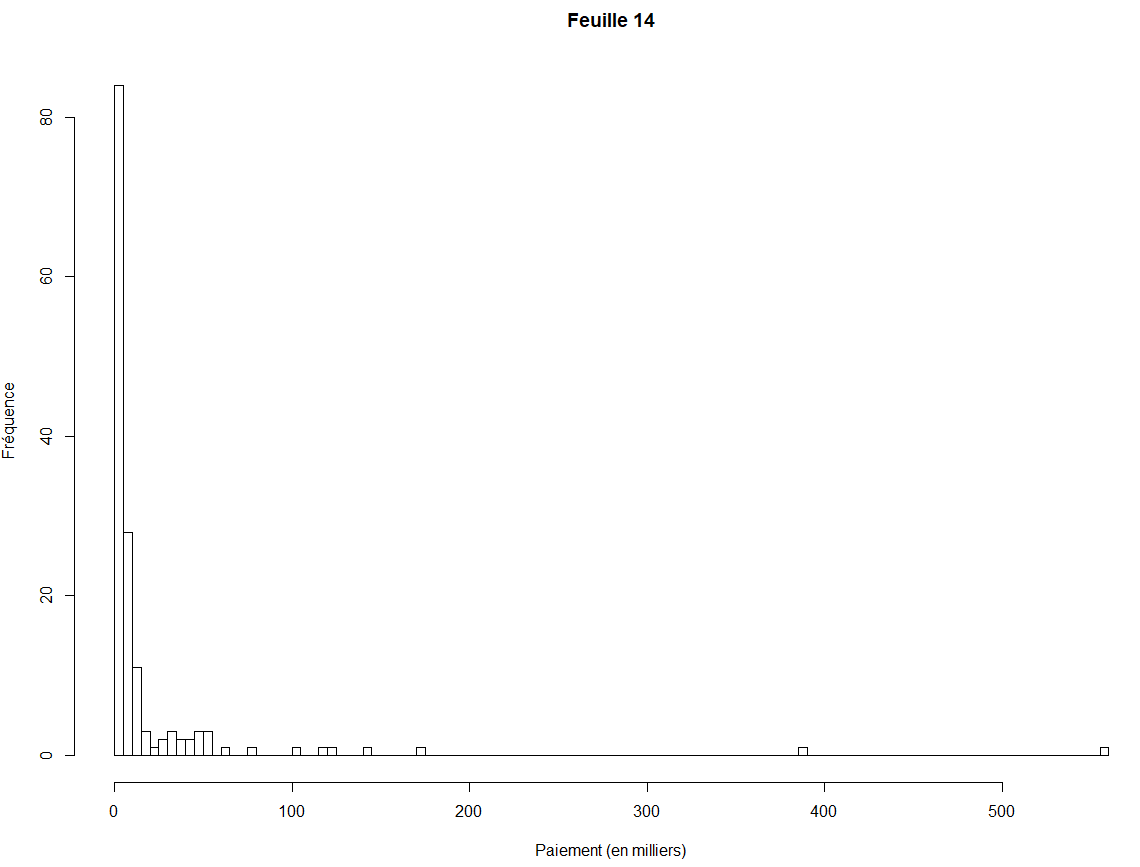
\includegraphics[width=.90\textwidth]{Fig_14.PNG}}
   \label{pai_23}
\end{figure}
}

\frame{
\frametitle{Conclusion}
\begin{itemize}
    \fleche Est-ce que les arbres de décisions sont une option viable à l'approche paramétrique?
    \pause
    \begin{itemize}
        \item (+) Facile à ajouter dans l'algorithme de simulation.
        \pause
        \item (+) Intuitif à comprendre.
        \pause
        \item (+) Résultats similaires à ceux du modèle MLG quand la base de données ne pose pas de problèmes.
    \end{itemize}
    \pause
    \begin{itemize}
        \item (-) Si valeurs aberrantes présentes, les arbres de décisions ne sont pas assez robustes pour mitiger l'influence de ces valeurs. Accentuer avec l'ajout de la composante d'ajustement univariée.
        \pause
        \item (-) Augmente la volatilité de la distribution de réserve.
    \end{itemize}
\end{itemize}
}

\frame{
\frametitle{Conclusion}
\begin{itemize}
    \fleche Prometteurs, mais plusieurs autres aspects doivent être étudiés avant que ceux-ci soient réellement utilisés dans le milieu pratique.
    \pause
    \fleche Lorsque le nombre de simulations augmente, avons-nous une distribution qui devient semblable à celle du modèle avec MLG?
    \pause
    \fleche Avec une base de données ayant des covariables avec des effets d'interactions, est-ce que les modèles avec arbres de décisions sont plus efficaces que les modèles avec MLG?
    \pause
    \fleche Est-ce que l'utilisation d'une plus grande panoplie de distributions pour le modèle avec ajustement univarié peut améliorer de façon significative la distribution des réserves?
\end{itemize}
}

\frame{
\frametitle{Conclusion}
\begin{itemize}
    \fleche Prometteurs, mais plusieurs autres aspects doivent être étudiés avant que ceux-ci soient réellement utilisés dans le milieu pratique.
    \item Est-ce que l'utilisation des forêts aléatoires pourrait être ajoutée dans l'algorithme?
    \begin{itemize}
        \cercle Réalisation d'une loi uniforme $[0,1]$.
        \cercle Trouver le quantile empirique des paiements sachant la feuille pour chaque arbre.
        \cercle Moyenne du vecteur de quantile pourrait ensuite être utilisée comme réalisation de paiement.
    \end{itemize}
\end{itemize}
}

\frame{
\frametitle{Références}
\tiny
\begin{itemize}
    \item[] Antonio, K., Plat, R., 2014. Micro-level stochastic loss reserving for general insurance. Scand. Actuar. J. 2014 (7), 649–669.
    \item[] Arjas, E., 1989. The claims reserving problem in non-life insurance: Some structural ideas. ASTIN Bull. 19 (2), 139–152.
    \item[] Avanzi, B., Wong, B., Yang, X., 2016. A micro-level claim count model with overdispersion and reporting delays. Insurance : Mathematics and Economics (71), 1-14.
    \item[] Breiman, L., Friedman, J., Olshen, R. A., Stone, C. J., 1984. Classification and Regression Trees. Chapman and Hall. 
    \item[] Duval, F., Pigeon, M., 2019. Individual loss reserving using a gradient boosting-based approach. Risks 7 (79), 1-18.
    \item[] Grenier, M., 2019. Travail 2 : Antionio & Plat (2014) - Application d’un modèle de réserve individuel. UQAM, 1-14.
    \item[] Kuo, K., 2019. DeepTriangle: A deep learning approach to loss reserving. Risks 7(3) 97, 1-13.
    \item[] Lopez, O., 2019. A censored copula model for micro-level claim reserving. Insurance : Mathematics and Economics (87), 1-14.
    \item[] Lopez, O., Milhaud, X., Thérond, P-E., 2019. A tree-based algorithm adapted to microlevel reserving and long development claims. ASTIN Bull. 49(3), 741-762. 
    \item[] Lopez, O., Milhaud, X., Thérond, P-E., 2016. Tree-based censored regression with application in insurance. Electronic Journal of Statistics (10), 2685-2716.
    \item[] Norberg, R., 1993. Prediction of outstanding liabilities in non-life insurance. ASTIN Bulletin 23 (1), 95–115. 
    \item[] Norberg, R., 1999. Prediction of outstanding liabilities - ii model variations and extensions. ASTIN Bulletin 29 (1), 5–27.
    \item[] Pigeon, M., 2019. MAT9594: Note de cours numéro 7 sur les arbres de décisions. UQAM.
    \item[] Reynkens, T., Roel, V., Beirlant, J., Antonio, K., 2016. Modeling censored losses using splicing : A global fit strategy with mixed erlang and extreme value distributions. SSNR Electronic Journal. 1-29.
    \item[] Wüthrich, M. V., 2018. Machine learning in individual claims reserving. Scandinavian Actuarial Journal (6), 465-480.
    \item[] Wüthrich M. V., Gabrielli, A., 2018. An individual claims history simulation machine. Risks 6 (29),1–32.
\end{itemize}
}


% ------------------------------------------------------------------------------------------------------------------------------

\end{document}
